%%%%%%%%%%%%%%%%%%%%%%%%%%%%%%%%%%%%%%%%%%%%%%%%%%%%%%%%%%%%%%%%%%%%%%  
%%%%%%%%%%%   Zastosowanie głębokich sieci neuronowych do detekcji 
%%%%%%%%%%             budynków na zdjęciach lotniczych                   
%%%%%%%%%%                     Mateusz Gomulski                               
%%%%%%%%%%%%%%%%%%%%%%%%%%%%%%%%%%%%%%%%%%%%%%%%%%%%%%%%%%%%%%%%%%%%%%
\documentclass[left=2.5cm, right=2.5cm, top=2.5cm, bottom=3cm, bindingoffset=6mm, nohyphenation=false]{Pakiety/thesis}

\langpol
\graphicspath{{Obrazy//}}
\addbibresource{Bibliografia//bibliografia.bib}

\begin{document}
%---------------------------------------------------------------
% Strona tytułowa
%---------------------------------------------------------------
\Thesis
\instytut{Radioelektroniki i Technik Multimedialnych}
\kierunek{Głębokie Sieci Neuronowe – Zastosowania w Mediach Cyfrowych}
\title{Zastosowanie głębokich sieci neuronowych do detekcji budynków na zdjęciach lotniczych}
\engtitle{Buildings detection in aerial images using deep neural networks}
\author{Mateusz Gomulski}
\promotor{prof. dr hab. inż. Władysław Skarbek}
\date{\the\year}
\maketitle

%---------------------------------------------------------------
% Streszczenie po polsku
%---------------------------------------------------------------
\clearpage
\streszczenie 
Niniejsza praca dyplomowa podejmuje problematykę detekcji budynków na zdjęciach lotniczych przy wykorzystaniu głębokich sieci neuronowych. Zastosowana konwolucyjna sieć neuronowa o~nazwie \textit{GML-Net} posiada architekturę typu \textit{U-Net} z~enkoderem wywodzącym się z~rodziny \textit{ResNet} oraz z blokami \textit{BottleNeck} zapewniającymi odczyt i~agregację map cech z~przekroju różnych skal. Wykorzystane w~bieżącej pracy punktowo i~wgłębnie separowalne konwolucje pozwalają sieci neuronowej efektywnie nauczyć się korelacji kanałów przestrzennych, uniknąć nadmiernego dopasowania oraz uzyskać większą efektywność obliczeniową. Jako funkcję straty zapewniającą efektywne uczenie się sieci, zdecydowano się użyć ważonej sumy \textit{Binary Cross-Entropy Loss}, \textit{Dice Loss} oraz \textit{Lovász hinge loss}. Niniejsza praca dyplomowa pokazuje, iż tak zbudowana sieć neuronowa pozwala uzyskać zadowalające wyniki przy zdjęciach lotniczych zawierających zaledwie trzy kanały przestrzenne (RGB). Wyniki te są tylko nieznacznie gorsze od wyników uzyskanych przez najlepsze modele wytrenowane na zbiorze danych \textit{Inria Aerial Image Labeling Dataset}.
\slowakluczowe Głębokie sieci neuronowe, Zdjęcia lotnicze, Rozpoznawanie budynków, Segmentacja semantyczna, \textit{ResNet}, \textit{U-Net}, \textit{BottleNeck}

%---------------------------------------------------------------
% Streszczenie po angielsku
%---------------------------------------------------------------
\newpage
\abstract 
The diploma thesis deals with the problem of detecting buildings in aerial images using deep neural networks. The \textit{GML-Net} convolutional neural network that is used in this work has a \textit{U-Net} architecture with an encoder derived from the \textit{ResNet} family and \textit{BottleNeck} blocks that provide reading and aggregation of feature maps from a~cross-section of various scales. Pointwise and depthwise convolutions used in this diploma thesis allow neural network to effectively learn spatial channel correlation, avoid overfitting and obtain greater computational efficiency. Effective network learning is ensured by loss function defined as a~weighted sum of \textit{Binary Cross-Entropy Loss}, \textit{Dice Loss} and \textit{Lovász hinge Loss}. This diploma thesis shows that a~neural network constructed in such a~way allows to obtain satisfactory results for aerial images with only three spectral channels (RGB). These results are only slightly worse than the results achived by the best models trained on the \textit{Inria Aerial Image Labeling Dataset}.
\keywords Deep neural networks, Aerial images, Buildings detection, Semantic segmentation, \textit{ResNet}, \textit{U-Net}, \textit{BottleNeck}
\pagestyle{plain}

%---------------------------------------------------------------
% Spis treści
%---------------------------------------------------------------
\cleardoublepage
\tableofcontents

%---------------------------------------------------------------
% Rozdziały
%---------------------------------------------------------------
\clearpage
\pagestyle{headings}
\section{Wstęp}

Głębokie uczenie zrewolucjonizowało dziedzinę przetwarzania sygnałów cyfrowych w~niespotykanej dotąd skali. Przed erą głębokich sieci neuronowych komputery nie były w~stanie zbliżyć się do skuteczności z~jaką przeciętny człowiek radzi sobie z~takimi zagadnieniami z~dziedziny cyfrowego przetwarzania sygnałów jak na przykład: rozpoznawanie / segmentacja obiektów na zdjęciach cyfrowych, rozpoznawanie pozy / emocji na podstawie analizy filmu wideo czy detekcja poleceń / słów kluczowych na podstawie nagrania audio. Nadejście ery głębokich sieci neuronowych, której początek można datować na 2006 rok (a intensywny rozwój na czas po 2012 roku), spowodowało nie tylko dorównanie przez komputery, w~wielu zadaniach, średniej ludzkiej skuteczności, ale często istotne przewyższenie jej (ang. \emph{superhuman performance}). Dobrym przykładem ponadludzkiej skuteczności głębokich sieci neuronowych jest konkurs \emph{ImageNet Large Scale Visual Recognition Challenge (ILSVRC)}, który polegał na automatycznym generowaniu podpisów do obrazów znajdujących się w zbiorze \emph{ImageNet}. Jeszcze w~2011~roku zwycięskie rozwiązanie w~tym konkursie charakteryzowało się stopą błędów top-5\footnote{Stopa błędów top-5 to miara stosowana przy ocenie modeli klasyfikacji w~ramach uczenia maszynowego, zakłada ona, że model zakwalifikował dany obraz poprawnie gdy wśród pięciu najbardziej prawdopodobnych kategorii wskazanych przez model znajduje się poprawna kategoria} na poziomie 26\%. Przełomowe rozwiązanie zaproponowane przez Krizhevsky A., Sutskever I. i Hinton G. z~2012~roku \cite{alexnet}, wykorzystujące głębokie uczenie się, wygrało ten konkurs osiągając stopę błędów top-5 na poziomie 15\%. W~2017 roku organizatorzy konkursu \emph{ILSVRC} zapowiedzieli zakończenie jego organizacji (przy najlepszym wyniku top-5 równym 2,251\% uzyskanym przez sieć \emph{SENet}), gdyż rezultaty osiągane na zbiorze testowym przez większość zgłaszanych do konkursu modeli zaczęły istotnie przekraczać wyniki przeciętnego człowieka (koło 5\%) - zapowiedzieli oni jednoczenie organizację dużo bardziej wymagającego konkursu wiążącego się z klasyfikacją trójwymiarowych obiektów.

Generowanie automatycznych podpisów do zdjęć jest jednak zadaniem dużo mniej skomplikowanym niż detekcja obiektów na zdjęciach lotniczych czy też satelitarnych. Jest tak, gdyż zdjęcia lotnicze / satelitarne charakteryzują się o~wiele większą złożonością pod względem skali, jakości, rozdzielczości czy też zaszumienia niż zdjęcia pochodzące z~takich zbiorów jak \emph{ImageNet} a~głównym zadaniem sieci nie jest wybranie jednego z~tysiąca podpisów, ale wskazanie piksel po pikselu, do jakiego obiektu dany piksel z~konkretnego zdjęcia należy. Stąd też rezultaty osiągane przez głębokie sieci neuronowe przy tego typu zadaniach są w~dalszym ciągu dużo gorsze niż rezultaty osiągane przez człowieka. Biorąc pod uwagę stale wzrastającą liczbę zdjęć oraz nagrań wideo rejestrowanych codziennie przez satelity / samoloty / drony, śmiało można stwierdzić, iż istnieje duże zapotrzebowanie / pole do rozwoju i~ulepszeń głębokich metod stosowanych do analizy tego typu danych, tak żeby w przyszłości głębokie sieci neuronowe mogły z~ powodzeniem zastąpić w~tym obszarze człowieka. W~szczególności, istotną kwestią przy analizie zdjęć lotniczych i satelitarnych, jest detekcja budynków, gdyż świadomość dokładnego położenia zabudowań na mapach miast jest niezbędna w~takich dziedzinach życia społeczno-ekonomicznego jak: urbanistyka, socjologia, bezpieczeństwo publiczne, ubezpieczenia majątkowe czy też reagowanie kryzysowe w obliczu klęsk żywiołowych.

Niniejsza praca podejmuje problematykę rozpoznawania budynków na zdjęciach lotniczych przy pomocy głębokich sieci neuronowych, gdzie jako zbiór testowy wykorzystywany jest zbiór \emph{Inria Aerial Image Labeling Dataset}. Sieć neuronowa przedstawiona w~niniejszej pracy korzysta z~architektury typu \emph{U-Net}, jej enkoder jest zasilany wagami modelu \emph{Wide ResNet-50-2} \cite{zagoruyko}, całość łączą bloki typu \emph{Bottleneck} (w~wersji OSNet \cite{zhou}) gwarantujące agregację map cech z~przekroju różnych skal. Aby efektywnie nauczyć się korelacji kanałów przestrzennych, uniknąć nadmiernego dopasowania oraz uzyskać większą efektywność obliczeniową, zaimplementowana sieć neuronowa wykorzystuje punktowo i~wgłębnie separowalne konwolucje. Efektywność głębokiego uczenia się jest gwarantowana przez funkcję straty złożoną z~ważonej sumy: Binary Cross-Entropy Loss, Dice Loss oraz Lovász hinge loss. W~kolejnych rozdziałach niniejszej pracy opisywane są podstawy teoretyczne głębokich sieci neuronowych, analizowana jest literatura dotycząca detekcji budynków na zdjęciach lotniczych i~satelitarnych oraz szczegółowo definiowane są: architektura użytej sieci neuronowej, zbiór danych i~jego transformacje, funkcje strat oraz metody oceny skuteczności działania zaimplementowanej sieci. Całość zakończona jest porównaniem uzyskanych wyników z wynikami przedstawionymi w~literaturze.

\clearpage
\section{Podstawy teoretyczne głębokiego uczenia}

\subsection{Głębokie uczenie - podstawowe definicje}

Głębokie uczenie (ang. \emph{deep learning}) jest jedną z~najbardziej dynamicznie rozwijających się gałęzi sztucznej inteligencji (ang. \emph{artificial intelligence}). Zadaniem głębokiego uczenia jest wychwycenie jak największej liczby zależności (cech) występujących w~analizowanym zbiorze danych i~przedstawienie tych zależności w~prostszy sposób - przy pomocy sieci neuronowej z~odpowiednio dobranymi wagami. Głębokie uczenie można sklasyfikować jako podzbiór uczenia reprezentacji (ang. \emph{representation learning}), które z~kolei jest podzbiorem uczenia maszynowego (ang. \emph{machine learning}), a~to w~końcu stanowi podzbiór metod sztucznej inteligencji. Rysunek \ref{fig:diagram1} prezentuje diagram zależności pomiędzy wyżej wymienionymi dziedzinami.

\begin{figure}[!h]
    \centering \includegraphics[width=0.7\linewidth]{DL diagram.png}
    \captionsetup{format=hang}
    \caption{Diagram Venna ukazujący zależności pomiędzy głębokim uczeniem, uczeniem reprezentacji, uczeniem maszynowym a~sztuczną inteligencją \cite{goodfellow}}
    \label{fig:diagram1}
\end{figure}

Głębokie uczenie jest implementowane przy pomocy głębokich sieci neuronowych (ang. \emph{deep neural networks}), których architektura opiera się na połączonych ze sobą neuronach. Każde połączenie pomiędzy neuronami jest reprezentowane przy pomocy wagi, która wskazuje jak ważna jest wartość danego neuronu (w~konkretnym połączeniu z~innym neuronem) z~perspektywy całej sieci. Neurony są grupowane w~warstwy (w~liczbie zazwyczaj od kilku do nawet kilkuset), a~te z~kolei grupuje się w~bloki, czyli funkcjonalne jednostki przetwarzania danych. Głębokie sieci neuronowe są implementowane przy pomocy bardzo zróżnicowanych architektur jednak architektury te zazwyczaj składają się z~kilku podstawowych elementów (warstw). Do najważniejszych z~nich należą: warstwa konwolucyjna, warstwa liniowa, warstwa grupująca, warstwa aktywacji, warstwa \emph{dropout} oraz warstwa normalizacji partiami. Najbardziej popularnymi klasami głębokich sieci neuronowych są konwolucyjne sieci neuronowe (ang. \emph{convolutional neural networks}) oraz rekurencyjne sieci neuronowe (ang. \emph{recurrent neural networks}). Konwolucyjne sieci neuronowe charakteryzują się tym, iż ich architektura jest oparta o~warstwy splotowe, które pozwalają na efektywną ekstrakcję cech. Natomiast rekurencyjne sieci neuronowe charakteryzuje występowaniem cyklicznych połączeń pomiędzy neuronami, które umożliwiają analizę danych o~charakterze sekwencyjnym. 

\paragraph*{Warstwa konwolucyjna (splotowa)}

Warstwa konwolucyjna (ang. \emph{convolution layer}) jest podstawową jednostką przetwarzania w~głębokich sieciach neuronowych. Składa się ona z~szeregu filtrów (ang. \emph{filter} / \emph{kernel}), o~rozmiarach zazwyczaj nieprzekraczających kilku pikseli, które przesuwając się po danych wejściowych, reprezentowanych zazwyczaj w~formie wielowymiarowej macierzy, wykonują operację iloczynu Hadamarda, po którym następuje sumowanie wszystkich elementów uzyskanej macierzy do pojedynczych liczb (ekstrakcja cech). Liczby te następnie tworzą nową macierz, która jest nazywana mapą cech (ang. \emph{features map}). Każdy z~filtrów zastosowanych w~warstwie konwolucyjnej składa się początkowo z~losowych wartości, w~trakcie trenowania sieci, w~kolejnych iteracjach obliczeń (zwanych powszechnie epokami (ang. \emph{epochs})), następuje aktualizacja wartości filtrów, aby sieć nabierała pożądanych od niej własności. Każdy filtr warstwy splotowej tworzy własną mapę cech, więc deklarując liczbę filtrów w~danej warstwie, deklarujemy ile map cech (unikalnych atrybutów danego zbioru danych) na wyjściu z danej warstwy chcemy uzyskać. W~ramach warstwy konwolucyjnej, poza rozmiarem filtrów (ich kształtem), należy zdefiniować jeszcze kilka ważnych parametrów (hiperparametrów\footnote{Hiperparametrami sieci neuronowej nazywamy najważniejsze parametry tej sieci, które są definiowane przez jej architekta przed przystąpieniem do procesu trenowania.}), takich jak: 
\begin{itemize}
\item krok (ang. \emph{stride}) o~jaki filtr będzie przesuwany w~czasie ekstrakcji cech,
\item \emph{padding} czyli wskazanie czy chcemy by tworzone mapy cech utrzymały rozdzielczość danych wejściowych, jeśli tak to jakimi wartościami należy uzupełnić ewentualne braki powstałe na skutek różnic pomiędzy rozmiarem danych wejściowych a~rozmiarem filtra (domyślnie braki są uzupełniane wartością zero),
\item dylacja (ang. \emph{dilation}) czyli odległość pomiędzy punktami filtra - domyślnie filtr jest nakładany na sąsiadujące ze sobą elementy macierzy wejściowej, ale można przy pomocy dylacji ustawić by był on nakładany na przykład na co drugi jej element (dylacja równa 2).
\end{itemize}

Szczególnym przypadkiem warstwy konwolucyjnej jest \textbf{konwolucja transponowana} (ang. \emph{transposed convolution}), którą można określić jako operację odwrotną do operacji splotu. O~ile celem konwolucji jest uzyskanie uproszczonej reprezentacji danych wejściowych, o tyle konwolucja transponowana stara się przetransformować dane wejściowe o~mniejszej wymiarowości,, do danych o~większym wymiarze. Stąd też konwolucję transponowaną często określa się jako nadpróbkowanie (ang. \emph{upsampling}) i~jest ona najczęściej wykorzystywana przy zadaniach związanych z rekonstrukcją danych. Innym szczególnym przypadkiem warstwy konwolucyjnej jest \textbf{konwolucja z~filtrem o rozmiarze 1x1}, której najczęstszym zadaniem jest redukcja liczby map cech w~danym miejscu sieci neuronowej, dzięki czemu dochodzi do istotnego zmniejszenie rozmiaru tej sieci bez dużego uszczerbku dla jej efektywności. 

\paragraph*{Warstwa liniowa}

Warstwa liniowa (ang. \emph{linear layer} / \emph{dense layer} / \emph{fully-connected layer}) to najprostsza ze wszystkich warstw stosowanych w~głębokich sieciach neuronowych. Jej zadaniem jest zastosowanie transformacji liniowej na danych pochodzących z~poprzedzającej ją warstwy. Hiperparametrami warstwy liniowej są: liczba wejść (ang. \emph{input size}), liczba wyjść (ang. \emph{output size}) oraz flaga wskazująca czy przy przeprowadzaniu transformacji linowej należy stosować przesunięcie (ang. \emph{bias}).

\paragraph*{Warstwa grupująca}

Warstwa grupująca (ang. \emph{pooling layer}) to jednostka, której zadaniem jest redukcja wymiarowości danych wejściowych poprzez zastosowanie wybranej funkcji grupującej (najczęściej funkcji maximum lub funkcji średniej). Podobnie jak w przypadku warstwy splotowej, po danych wejściowych warstwy grupującej przesuwany jest filtr o~wymiarach kilku pikseli, którego zadaniem jest wybranie największej wartości z~danego zakresu danych (\emph{max pooling}) lub wyliczenie średniej dla tego zakresu (\emph{average pooling}). W~ten sposób, dla filtra (okna) warstwy grupującej o~wymiarach na przykład 2x2, cztery wartości danych wejściowych są redukowane do jednej wartości - maksimum lub średniej z~nich. W~ramach warstwy grupującej definiowany jest taki sam zbiór hiperparametrów jak w~przypadku warstwy konwolucyjnej czyli: rozmiar filtra, krok filtra, \emph{padding} oraz~dylacja - mają one dokładnie takie samo zastosowanie jak w~przypadku warstwy splotowej. Poza zdefiniowanymi powyżej podstawowymi operacjami grupującymi często wyróżnia się jeszcze operację globalnego grupowania do maksimum (ang. \emph{global max pooling}) oraz operację globalnego grupowania do średniej (ang. \emph{global average pooling}), które polegają na zastosowaniu funkcji maksimum / średniej nie na poziomie filtrów, ale na poziomie całych kanałów danych wejściowych. 

\paragraph*{Warstwa aktywacji}

Warstwa aktywacji (ang. \emph{activation function}) przetwarza dane pochodzące z~map cech wygenerowanych w~poprzednich warstwach po to by nadać im niezbędną nieliniowość. Jest ona konieczna po to by sieci neuronowe były w~stanie nauczyć się skomplikowanych wzorców występujących w~analizowanych przez nie danych. Do najpopularniejszych warstw (funkcji) aktywacji wykorzystywanych w~głębokich sieciach neuronowych można zaliczyć:

\begin{itemize}
\item \emph{sigmoid}:
 \begin{equation}
simg(x) = \frac{1}{1 + e^{-x}}
\end{equation}
\item \emph{tangens hiperboliczny}: 
 \begin{equation}
tanh(x) = \frac{e^x-e^{-x}}{e^{x}+e^{-x}}
\end{equation}
\item \emph{ReLU}:
 \begin{equation}
 ReLU(x) = max(x, 0)
\end{equation}
\item \emph{Leaky ReLU}:
 \begin{equation}
  LReLU(x) = 
 \begin{cases}
  x & \text{dla x > 0}  \\
  0,01 \cdot x & \text{dla x $\leq$ 0} \\
  \end{cases}
\end{equation}
\item \emph{Parametric ReLU}:
 \begin{equation}
 PReLU(x) =  
 \begin{cases}
  x & \text{dla x > 0}  \\
  \alpha \cdot x & \text{dla x $\leq$ 0} \\
  \end{cases}
\end{equation}
\item \emph{Exponential Linear Unit}:
 \begin{equation}
 ELU(x) = 
  \begin{cases}
  x & \text{dla x >  0}  \\
  \alpha \cdot (e^{x}-1)  & \text{dla x $\leq$ 0} \\
  \end{cases}
\end{equation}
\item \emph{softmax\footnote{Softmax jest specyficzną funkcją aktywacji, gdyż jej głównym zadaniem jest normalizacja danych wyjściowych sieci neuronowej do rozkładu prawdopodobieństwa}}:
 \begin{equation}
 softmax(x_i) = \frac{e^{x_i}}{\sum_{j=1}^{n}e^{x_j}}
\end{equation}
\end{itemize}

Funkcje \emph{sigmoid} oraz \emph{tangens hiperboliczny}, ze względu na swoją złożoność obliczeniową i~fakt, iż mogą się przyczyniać do występowania problemu zanikającego gradientu, są stosunkowo rzadko wykorzystywane w~bieżących architekturach głębokich sieci neuronowych. Najczęściej stosowaną funkcją aktywacji jest \emph{ReLU}, głównie ze względu na swoją prostotę i~skuteczność. Często zarzuca się jej jednak brak różniczkowalności w~punkcie 0 oraz zerową wartość pochodnej dla ujemnych argumentów, która może powodować wymieranie neuronów (\emph{dead ReLU}). Stąd też opracowane zostały różne modyfikacje funkcji ReLU, które starają się rozwiązać te problemy przy okazji zachowując wszystkie najważniejsze zalety tej funkcji aktywacji (\emph{Leaky ReLU}, \emph{Parametric ReLU}, \emph{Exponential Linear Unit}).

\paragraph*{Warstwa \emph{dropout}}

Głębokie sieci neuronowe ze względu na ogromną liczbę trenowalnych parametrów (wag) są szczególnie podatne na problem zwany przeuczeniem (ang. \emph{overfitting}), który polega na zbyt dokładnym dopasowaniu się sieci neuronowej do konkretnych danych uczących, przez co sieć ta staje się mniej skuteczna w~generowaniu prawidłowych predykcji dla danych z~poza zbioru uczącego (rośniej jej błąd generalizacji). Zadaniem warstwy \emph{dropout} jest zmiana funkcjonowania sieci neuronowej w~taki sposób by jak najbardziej zminimalizować błąd generalizacji modelu. Rozwiązaniem tego problemu, uzyskiwanym w~ramach warstwy \emph{dropout}, jest losowe wyłączanie (zerowanie aktywacji) niektórych neuronów sieci w~każdej epoce jej uczenia, po to by miała ona zdolność wyłapywania jak najbardziej uniwersalnych cech danego zbioru danych, niezwiązanych z~konkretnymi wartościami poszczególnych neuronów. To jaki procent wszystkich neuronów zostanie wyłączonych w~konkretnej epoce jest definiowane przy pomocy hiperparametru \emph{p}, czyli prawdopodobieństwa, że dany neuron zostanie wyzerowany. 

Warstwę \emph{dropout} w~związku z~jej właściwością zapobiegania przeuczeniu sieci neuronowej nazywa się często techniką regularyzacji. Inną równie często stosowaną techniką regularyzacji modelu jest \textbf{augmentacja danych} (ang. \emph{data augmentation}), czyli technika transformacji danych treningowych sieci neuronowej w~taki sposób by jak najbardziej je zróżnicować, uzyskując tym samym większą liczbę przypadków uczących. Jednymi z~najpopularniejszych sposobów przekształcania danych uczących są: skalowanie (ang. \emph{scale}), przesuwanie (ang. \emph{shift}), losowe obracanie (ang. \emph{random rotation}), losowe wycinanie fragmentów (ang. \emph{random crop}) czy normalizacja (ang. \emph{normalization}). 

\paragraph*{Warstwa normalizacji partiami}

Zadaniem warstwy normalizacji partiami (ang. \emph{batch normalization layer}) jest zaradzenie problemowi ciągłej zmiany rozkładów wartości generowanych przez poszczególne warstwy głębokich sieci neuronowych wraz z~postępem ich uczenia. W~związku z~tym zjawiskiem poszczególne warstwy modelu dużą część swojej pracy poświęcają na dostosowanie się do wewnętrznego przesunięcia rozkładów (ang. \emph{internal covariate shift}), zamiast spożytkować tę pracę na efektywną naukę. Rozwiązaniem tego problemu było dodanie nowej warstwy do architektury modelu, której zadaniem była odpowiednia standaryzacja wartości wyjściowych z~poprzedniej warstwy poprzez odjęcie średniej wartości w~danej partii (ang. \emph{batch}) i~podzielenie przez odchylenie standardowe z~tej partii. Zastosowanie warstwy normalizacji partiami pozwala na efektywniejszą naukę sieci neuronowej - sieć w~czasie treningu szybciej minimalizuje funkcję strat.

\subsection{Ewolucja architektur głębokiego uczenia}

Termin głębokie uczenie zyskał w~ostatnim czasie ogromną popularność, głównie dzięki mnogości zastosowań jaką ta gałąź sztucznej inteligencji znalazła w~szerokiej gamie dziedzin życia codziennego - od samochodów autonomicznych, przez asystentki głosowe w~urządzeniach mobilnych / \emph{smart home}, aż po systemy rozpoznawania twarzy na lotniskach. Jednak termin ten nie jest nowy w~świecie nauki, był on używany przez naukowców od wielu lat, a~jego korzenie można datować na lata 40-ste dwudziestego wieku. 

\subsubsection{Cybernetyka (1943 - 1969)}
Praprzodkiem głębokiego uczenia, rozwijanym w~latach 40., 50. i~60. XX wieku, była cybernetyka, czyli nauka badająca mechanizmy kontroli i~komunikacji u~zwierząt i~maszyn \cite{wiener}. W~ramach cybernetyki naukowcy starali się stworzyć modele mogące naśladować biologiczną pracę mózgu. Najważniejszymi osiągnięciami tamtego okresy były następujące modele liniowe:

\begin{itemize}
\item \textbf{model neuronu} stworzony w~1943 roku przez Warrena McCullocha i~Waltera Pittsa (przez autorów nazywany \emph{Threshold Logic Unit}) \cite{mcculloch}, który oparty był na równaniu liniowym z~arbitralnie dobranymi wagami przy zmiennych wejściowych (patrz rysunek \ref{fig:neuron1}),

\begin{figure}[!h]
    \centering \includegraphics[width=0.6\linewidth]{Neuron.jpeg}
    \captionsetup{format=hang}
    \caption{Przykładowy schemat neuronu zaprezentowany w~1943 roku przez Warrena McCullocha i~Waltera Pittsa \cite{mcculloch}}
    \label{fig:neuron1}
\end{figure}

\item \textbf{model perceptronu} zaprezentowany w~1958 roku przez Franka Rosenblatta \cite{rosenblatt}, który był rozwinięciem neuronu o~możliwość samodzielnej nauki wartości wag przy poszczególnych zmiennych na podstawie danych treningowych\footnote{Wielu naukowców uznaje model perceptronu zaprezentowany przez Franka Rosenblatta za pierwszą współczesną sieć neuronową (\emph{feedforward neural network}).} (patrz rysunek \ref{fig:perceptron1}),

\begin{figure}[!h]
    \centering \includegraphics[width=1.0\linewidth]{Perceptron.jpeg}
    \captionsetup{format=hang}
     \caption{Schematyczna reprezentacja połączeń w~prostym perceptronie zaprezentowana w~1958 roku przez Franka Rosenblatta \cite{rosenblatt}}
    \label{fig:perceptron1}
\end{figure}

\item model adaptacyjnego neuronu liniowego stworzony przez Bernarda Widrowa i~Teda Hoffa, określany skrótem \textbf{ADALINE} (ang. \emph{Adaptive Linear Neuron}), który od perceptronu różnił się między innymi tym, że w~czasie uczenia jego wagi były dostosowywane do ważonej sumy wartości wejściowych (patrz rysunek \ref{fig:adaline1}).
\end{itemize} 

\vspace{1cm}

\begin{figure}[!h]
    \centering \includegraphics[width=0.8\linewidth]{ADALINE.jpeg}
    \captionsetup{format=hang}
      \caption{Schemat ADALINE zaprezentowany w 1960 roku przez Bernarda Widrowa i~Teda Hoffa \cite{widrow}}
    \label{fig:adaline1}
\end{figure}

Pod koniec lat 60. XX wieku popularność modeli tworzonych w~nurcie cybernetyki istotnie zmalała za sprawą licznych ograniczeń modeli liniowych wskazywanych przez część naukowców. W~1969 roku ukazała się słynna książka Marvina Minsky'ego i~Seymoura Paperta pod tytułem \emph{Perceptrons: an introduction to computational geometry} \cite{minsky}, która wskazywała na liczne ograniczenia modelu pojedynczego perceptronu Rosenblatta, takie jak na przykład fakt, iż nie jest on w~stanie nauczyć się prostej operacji logicznej \emph{XOR} (ani żadnej innej operacji nieseparowalnej liniowo). Minksy i~Papert wskazywali jednocześnie, iż takich operacji mogłaby nauczyć się sieć złożona z~kilku perceptronów, lecz nie ma efektywnych sposobów uczenia takich sieci. Ta publikacja istotnie przyczyniła się do spadku popularności modeli uczenia inspirowanych biologicznie. 

\subsubsection{Konekcjonizm (1980 - 1998)}

Kolejnym przodkiem głębokiego uczenia, który najdynamiczniej rozwijał się  w~latach 80. i~90. XX wieku, był konekcjonizm, czyli podejście z~dziedziny kognitywistyki, które miało za zadanie wyjaśnić zjawiska umysłowe przy pomocy modeli neuronowych. Główną ideą tego nurtu sztucznej inteligencji było przekonanie, iż duża liczba prostych jednostek obliczeniowych połączonych w~sieć może umożliwić uzyskanie inteligentnego zachowania u~maszyny. 

\paragraph*{Neocognitron}

Jednymi z~najważniejszych artykułów początkowej fazy konekcjonizmu były artykuły Kunihiko Fukushimy wprowadzające pojęcia \textbf{\emph{cognitronu}} \cite{fukushima1} i~\textbf{\emph{neocognitronu}} \cite{fukushima2}, czyli samoorganizującej się sieci neuronowej (wzorowanej na systemie widzenia ssaków), która jest w~stanie rozpoznawać wzorce według geometrycznego podobieństwa ich kształtu. \emph{Neocognitron} był rozwinięciem \emph{cognitronu} wprowadzającym do sieci neuronowej charakter splotowy, co pozwoliło na uniezależnienie odpowiedzi modelu od umiejscowienia wzorca.  

\begin{figure}[!h]
    \centering \includegraphics[width=0.9\linewidth]{Neocognitron.jpeg}
    \captionsetup{format=hang}
    \caption{Diagram pokazujący połączenia pomiędzy warstwami w~neocognitronie zaprezentowanym w~1980 roku przez Kunihiko Fukushimę \cite{fukushima2}}
    \label{fig:neocognitron1}
\end{figure}

\emph{Neocognitron} można więc uznać za jeden z~pierwszych modeli z~dziedziny \textbf{konwolucyjnych sieci neuronowych}. Składał się on z~sześciu warstw splotowych przeplatanych warstwami grupującymi (patrz rysunek \ref{fig:neocognitron1}). Wejściem do modelu \textit{neocognitronu} były obrazy o rozmiarach 16~x~16, a~każda warstwa splotowa zawierała 24 filtry o~wymiarach 5~x~5. Po wytrenowaniu model Fukushimy był w~stanie rozpoznać pięć cyfr („0”, „1”, „2”, „3”, „4”) i~cztery litery („X”, „Y”, „T”, „Z”).

\paragraph*{Recurrent Neural Network (RNN)}

Prace Fukushimy przyczyniły się do rozwoju konwolucyjnych sieci neuronowych, które dawały bardzo obiecujące wyniki w~dziedzinie analizy obrazu, jednak miały one ograniczony potencjał zastosowania w~dziedzinach, w~których liczy się analiza całych sekwencji danych, jak na przykład analiza mowy, dźwięku, wideo czy pisma odręcznego. Do tego typu zastosowań potrzebna jest sieć, która dysponuje wewnętrzną pamięcią, po to by móc wyłapywać zależności nie tylko wewnątrz bieżącego fragmentu danych, ale także pomiędzy kolejnymi pojawiającymi się sekwencjami. Głębokie sieci neuronowe, które posiadają taką własność, nazywamy \textbf{rekurencyjnymi sieciami neuronowymi}. Jednym z~pierwszych artykułów z nurtu konekcjonizmu, wprowadzających rekurencyjne połączenia do sieci neuronowych, i~w~ten sposób tworzących sieci z dynamiczną pamięcią, był artykuł \emph{Serial order: A parallel distributed processing approach} napisany w~1986~roku przez Michaela Irwina Jordana \cite{jordan}. 

\begin{figure}[!h]
    \centering \includegraphics[width=0.3\linewidth]{Jordan.png}
    \captionsetup{format=hang}
    \caption{Diagram pokazujący połączenia w~sieci rekurencyjnej zaprezentowanej w~1986 roku przez Michaela Irwina Jordana \cite{jordan}}
    \label{fig:jordan1}
\end{figure}

W~swoim artykule Jordan proponuje nowatorskie podejście, które umożliwia nauczenia się sekwencji zdarzeń przez sieć neuronową, gdzie każda ukryta komórka (ang. \emph{hidden cell}) otrzymuje swoje własne dane wyjściowe z~odpowiednim, ustalonym opóźnieniem (patrz rysunek \ref{fig:jordan1}).

\paragraph*{Backpropagation}

Dynamiczny rozwój konekcjonizmu nie byłby możliwy bez opracowania efektywnego \textbf{algorytmu wstecznej propagacji błędu} (ang. \emph{backpropagation algorithm}). Jako jego twórcę uznaje się Paula Werbosa, który opisał go już w~1974 roku w~swojej rozprawie doktorskiej. Jednak algorytm ten nie zyskał dużego rozgłosu aż do 1986~roku, kiedy to David Rumelhart, Geoffrey Hinton i~Ronald Williams w~swoim artykule \emph{Learning representations by back-propagating errors} \cite{rumelhart} pokazali zastosowanie algorytmu wstecznej propagacji błędu do trenowania \textbf{wielowarstwowego perceptronu} (ang. \emph{Multilayer Perceptron}).

\begin{figure}[!h]
    \centering \includegraphics[width=0.4\linewidth]{MLP.png}
    \captionsetup{format=hang}
      \caption{Schemat wielowarstwowego perceptronu zaprezentowany w 1986 roku przez Davida Rumelharta, Geoffreya Hintona i~Ronalda Williamsa \cite{rumelhart}}
    \label{fig:mlp1}
\end{figure}

 W~czasie treningu sieci neuronowej algorytm wstecznej propagacji błędu wylicza gradient funkcji strat w~odniesieniu do wag tej sieci przy pomocy reguły łańcuchowej (ang. \emph{chain rule}). Gradient ten jest wyliczany dla każdej warstwy sieci neuronowej poczynając od najgłębszych warstw przechodząc iteracyjnie ku warstwom początkowym. 


\paragraph*{LeNet-5}

Kontynuatorem koncepcji Kunihiko Fukushimy, który do wytrenowania splotowej sieci neuronowej o~architekturze wzorowanej na \emph{neocognitronie} zastosował algorytm wstecznej propagacji błędu przedstawiony przez Davida Rumelharta, Geoffreya Hintona i~Ronalda Williamsa, był francuski naukowiec Yann André LeCun. W~swoich dwóch artykułach \emph{Backpropagation Applied to Handwritten Zip Code Recognition} z~1989 roku \cite{lecun1} i~\emph{Gradient-based learning applied to document recognition} z~1998 roku \cite{lecun2} zaprezentował on konwolucyjną sieć neuronową, która była w~stanie z~zadowalającą, jak na tamten czas, skutecznością rozpoznawać znaki pisma odręcznego. Sieć z~1998 roku zyskała nazwę \textbf{\emph{LeNet-5}}, składała się z~około 60 tysięcy trenowalnych parametrów podzielonych na siedem warstw (cztery splotowo-grupujące i~trzy warstwy gęste) o~filtrach w~rozmiarze 5~x~5, a~jako wejście przyjmowała obrazy o~rozdzielczości 32~x~32~(patrz rysunek \ref{fig:lenet1}). Co ciekawe, żeby ograniczyć liczbę trenowanych parametrów / połączeń niektóre warstwy modelu LeCunna łączyły się jedynie z~wybranymi filtrami z~warstw poprzednich. 

\begin{figure}[!h]
    \centering \includegraphics[width=1.0\linewidth]{LeNet-5.jpeg}
    \captionsetup{format=hang}
    \caption{Architektura sieci \emph{LeNet-5} stworzona w~1998 roku przez Yanna LeCuna \cite{lecun2}}
    \label{fig:lenet1}
\end{figure}

Sieć \emph{LeNet-5} stała się kamieniem milowym w~rozwoju sieci neuronowych, w~szczególności konwolucyjnych sieci neuronowych, gdyż pokazała, iż wielowarstwowe modele mogą osiągać w~niektórych zastosowaniach lepsze rezultaty niż inne dostępne w~tamtym czasie techniki rozpoznawania pisma odręcznego. Artykuł Yanna LeCunna z~1998 roku przyczynił się również do powstania sprawdzonego schematu trenowania sieci neuronowej z~warstwami splotowo-grupującymi zakończonymi warstwami gęstymi, schemat ten w~kolejnych latach był wielokrotnie powielany i~rozszerzany przez wielu autorów, lecz zasadniczy trzon architektury splotowych sieci neuronowych pozostał praktycznie niezmieniony.

\paragraph*{Long Short-Term Memory (LSTM)}

Drugim kluczowym artykułem, który powstał u~schyłku konekcjonizmu był artykuł z~1997 roku zatytułowany \emph{Long short-term memory} napisany przez Seppa Hochreitera i~Jürgena Schmidhubera \cite{hochreiter}. Wprowadzał on nową architekturę \textbf{\emph{LSTM}} w~dziedzinie rekurencyjnych sieci neuronowych, która pozwalała rozwiązać istotny problem dotykający w~tamtym czasie sieci \emph{RNN}, a~mianowicie problem zanikającego gradientu (ang. \emph{vanishing gradient problem})\footnote{Problem zanikającego gradientu pojawia się gdy, po przekroczeniu pewnej głębokości (długości przetwarzanej sekwencji), sieci neuronowe nie są w~stanie efektywnie uczyć się (aktualizować swoich wag), gdyż gradient błędów dla głębokich warstw (odległych sekwencji) staje się zbyt mały.}. Sieć \emph{LSTM} wprowadzała wewnętrzne mechanizmy zwane bramkami (ang. \emph{gates}), które pozwalały kontrolować przepływ informacji przetwarzanych przez sieć neuronową. Bramki te razem z~komórkami pamięci (ang. \emph{memory cells}) miały za zadanie nauczyć się, które informacje z~poprzednich sekwencji danych należy zatrzymać (uznając je za ważne), a~które można pominąć (nieważne). W~ramach modelu \emph{LSTM} wyróżniano trzy bramki:

\begin{itemize}
\item bramkę zapomnienia (ang. \emph{forget gate}) - bramka ta decydowała, którą informację należy zapomnieć, a którą zachować,
\item bramkę wejścia (ang. \emph{input gate}) - bramka ta aktualizowała wewnętrzny stan komórki pamięci,
\item bramkę wyjścia (ang. \emph{output gate}) - bramka ta decydowała jaki powinien być następny ukryty stan (ang. \emph{hidden state}) sieci. 
\end{itemize}

\begin{figure}[!h]
    \centering \includegraphics[width=0.9\linewidth]{LSTM.png}
    \captionsetup{format=hang}
    \caption{Architektura sieci \emph{LSTM} zaprezentowanej w~1997 roku przez Seppa Hochreitera i~Jürgena Schmidhubera \cite{hochreiter}}
    \label{fig:lstm1}
\end{figure}

Istotnymi ograniczeniami rozwoju sieci neuronowych tworzonych u~schyłku XX wieku były skromne, z~dzisiejszej perspektywy, zasoby obliczeniowe ówczesnych komputerów, które powodowały, iż wytrenowanie nawet najprostszej sieci neuronowej trwało wiele dni, stąd też metody stosowane przez przedstawicieli nurtu konektywizmu stopniowo traciły na popularności. 

\subsubsection{Głębokie uczenie (2006 - 2020)}

Za swoisty renesans nurtu konektywizmu i~właściwy początek głębokiego uczenia, można uznać rok 2006 kiedy to Hinton G., Osindero S. i Teh Y. W. w~swoim artykule \emph{A~Fast Learning Algorithm for Deep Belief Nets} \cite{hinton} pokazali, że sieci głębokiej wiarygodności mogą być efektywnie trenowane przy pomocy strategii o~nazwie chciwe warstwowe trenowanie wstępne (ang. \emph{greedy layer-wise pretraining}), która pozwalała zmniejszyć problem zanikającego gradientu oraz wzmocnić generalizację na zbiorze testowym poprzez efektywniejszą inicjalizację wag. Kolejni autorzy, wzorując się na pracy zespołu Geoffreya Hintona, szybko pokazali, że strategia chciwego warstwowego trenowania wstępnego może być zastosowana też do innych rodzajów głębokich sieci neuronowych, co otworzyło drogę do tworzenia modeli o~niedostępnych dotąd głębokościach.

\paragraph*{AlexNet}

W~tym samym czasie, dynamiczny rozwój przemysłu gier komputerowych i~związany z~nim rozwój kart graficznych, umożliwił bezprecedensowy wzrost efektywności trenowania głębokich sieci neuronowych - zamiast tradycyjnego trenowania sieci na jednostkach CPU (ang. \emph{central processing unit}) zaczęto je trenować na jednostkach GPU (ang. \emph{graphics processing unit}). Przełomowym artykułem w~zakresie trenowania modelu na wielu kartach graficznych był artykuł \emph{ImageNet classification with deep convolutional neural networks} opublikowany w~2012 roku przez Krizhevsky A., Sutskever I.  i~Hinton G. \cite{alexnet}. Co prawda nie był to pierwszy artykuł ukazujący ogromne możliwości GPU w~zakresie trenowania głębokich sieci neuronowych\footnote{Pierwszym takim artykułem był \emph{High Performance Convolutional Neural Networks for Document Processing} napisany w~2006 roku przez Chellapilla K., Puri S. i~Simard P.}, jednak stał się jednym z~najczęściej cytowanych artykułów w~dziedzinie głębokiego uczenia, gdyż łączył w~sobie wiele innowacyjnych na tamten czas rozwiązań takich jak:

\begin{itemize}
\item trening sieci na ogromnym zbiorze danych - \emph{ImageNet} z~15 milionami podpisanych obrazów dla ponad 22 tysięcy kategorii,
\item architektura modelu w~postaci konwolucyjnej sieci neuronowej, 
\item trening sieci neuronowej jednocześnie na dwóch kartach graficznych,
\item \emph{ReLU} jako funkcja aktywacji przyspieszająca zbieżność procesu uczenia, 
\item augmentacja danych treningowych realizowana poprzez translację, obroty horyzontalne i~wycinanie fragmentów obrazów, 
\item zastosowanie warstw \emph{dropout} w~celu zapobiegnięcia przetrenowaniu sieci,
\item trenowanie modelu w~pakietach przy użyciu stochastycznego spadku gradientu (ang. \emph{batch stochastic gradient descent}) z~jasno określonymi parametrami momentum i~spadku wagi (ang. \emph{weight decay}).
\end{itemize}

\begin{figure}[!h]
    \centering \includegraphics[width=1.0\linewidth]{AlexNet.jpeg}\
    \captionsetup{format=hang}
    \caption{Architektura sieci \emph{AlexNet} zaprezentowana w~2012 roku przez Alexa Krizhevsky'ego, Ilya Sutskevera i Geoffrey'a Hintona \cite{alexnet}}
    \label{fig:alexnet1}
\end{figure}

Sieć stworzona przez Krizhevsky'ego, Sutskevera i~Hintona  swoją architekturą bardzo przypominała sieć \emph{LeNet-5}, była jednak od niej wielokrotnie większa pod względem liczby parametrów. Składała się ona bowiem z~około 60 milionów trenowalnych parametrów podzielonych na osiem warstw (pięć warstw konwolucyjno-grupujących i~trzy warstwy gęste) o~filtrach rozmiarów 11 x 11, a~jako wejście przyjmowała obrazy RGB o~rozdzielczości 224~x~224 (patrz rysunek \ref{fig:alexnet1}). Sieć ta jest obecnie powszechnie znana pod nazwą \textbf{\emph{AlexNet}} (od imienia jej głównego autora), wygrała ona w~2012 roku prestiżowy konkurs \emph{ImageNet Large Scale Visual Recognition Challenge} pokonując drugi najlepszy model o~ponad 10~punktów procentowych (pod kątem stopy błędów top-5), zapoczątkowując tym samym swoistą rewolucję w dziedzinie głębokiego uczenia.

\paragraph*{VGGNet}

Kolejnym istotnym modelem z~perspektywy rozwoju głębokich sieci neuronowych był model \textbf{\emph{VGGNet}} zaprojektowany w~2014 roku przez Karen Simonyan i Andrew Zissermana. W~swoim artykule \emph{Very deep convolutional networks for large-scale image recognition} \cite{simonyan} zaproponowali oni konwolucyjną sieć neuronową o~niespotykanej dotąd głębokości liczącej 19 warstw i~o~filtrach wielkości 3 x 3 (patrz rysunek \ref{fig:vggnet1}). Użycie tak małych filtrów, autorzy argumentowali tym, iż zastosowanie modułu składającego się z~trzech filtrów 3 x 3, ma efektywne pole postrzegania jak jeden filtr 7 x 7, za to wymaga zdecydowanie mniejszej liczby trenowalnych parametrów i~pozwala zastosować trzykrotnie funkcję aktywacji. Pomimo tych zabiegów sieć \emph{VGGNet} posiadała bardzo duże rozmiary - składała się bowiem z~około 144 milionów trenowalnych parametrów.

\begin{figure}[!h]
    \centering \includegraphics[width=1.0\linewidth]{VGGNet.png}
    \captionsetup{format=hang}
    \caption{Architektura sieci \emph{VGGNet} zaprezentowana w~2014 roku przez Karen Simonyan i~Andrew Zissermana \cite{simonyan}}
    \label{fig:vggnet1}
\end{figure}

\paragraph*{GoogleNet}

Sieć \emph{VGGNet} zajęła drugie miejsce w~konkursie \emph{ImageNet Large Scale Visual Recognition Challenge 2014} osiągając stopę błędów top-5 na poziomie 7,32\%. Pierwsze miejsce w~tym konkursie zajęła sieć \textbf{\emph{GoogleNet}}, osiągając wynik równy 6,67\%. Sieć ta została zaproponowana w~październiku 2014 roku przez Szegedy Ch., Liu W., Jia Y., Sermanet P., Reed S., Anguelov D., Erhan D., Vanhoucke V., Rabinovich A. w~artykule \emph{Going deeper with convolutions}. Do momentu powstania \emph{GoogleNet} większość głębokich sieci neuronowych była realizowana przy pomocy sekwencyjnego nakładania na siebie warstw splotowych i~grupujących, sieć zaprojektowana przez pracowników \emph{Google Inc.} jako pierwsza wprowadziła przetwarzanie równoległe realizowane w blokach \emph{Inception}. Bloki te były realizowane jako równolegle warstwy konwolucyjne o~filtrach różnych rozmiarów (\textit{1x1}, \textit{3x3}, \textit{5x5}), których wynik był scalany (przy pomocy operacji konkatenacji) w~jedną warstwę na wyjściu z~danego bloku (patrz rysunek\ref{fig:inception1}). Zastosowanie w~blokach \emph{Inception} filtrów o~kilku różnych rozmiarach miało umożliwić detekcję cech o~dużym zróżnicowaniu przestrzennym. Zastosowanie filtrów  \textit{3x3}~służyło redukcji złożoności sieci, dzięki czemu finalny model zawierał około pięć milionów trenowalnych parametrów, czyli mniej więcej 12~razy mniej niż dużo mniej efektywna sieć \emph{AlexNet} z~2012 roku. Cała architektura modelu \emph{GoogleNet} składała się z~22~połączonych ze sobą sekwencyjnie bloków, z~czego dziewięć stanowiły moduły \emph{Inception}, łącznie w~całej sieci można było wyróżnić około 100~różnych warstw (patrz rysunek \ref{fig:googlenet1}).

\begin{figure}[!h]
    \centering \includegraphics[width=0.8\linewidth]{Inception1.jpeg}
    \centering \includegraphics[width=0.8\linewidth]{Inception2.jpeg}
    \captionsetup{format=hang}
    \caption{Architektura bloku \emph{Inception} zaprezentowana w~2014 roku w~artykule \emph{Going deeper with convolutions} \cite{szegedy}}
    \label{fig:inception1}
\end{figure}

 W~kolejnych latach autorzy modelu \emph{GoogleNet} wprowadzili liczne poprawki do opisywanej przez siebie architektury, dodali m.in. operację normalizacji partiami, faktoryzację konwolucji w~celu poprawienia efektywności obliczeniowej, usprawnili architekturę bloków \emph{Inception} poprzez dodanie połączeń \emph{residual connections} oraz zastosowali konwolucje separowalne wgłębnie (ang. \emph{depthwise separable convolutions}) i~punktowo (ang/ \emph{pointwise separable convolutions}) W~ten sposób powstały kolejne, jeszcze bardziej skuteczne, architektury wyrastające wprost z~\emph{GoogleNet} (zwanej też \emph{Inception-v1}), były nimi: \emph{Inception-v2} [2015], \emph{Inception-v3} [2015], \emph{Inception-v4} [2016] oraz \emph{Xception} [2017].

\newpage
\begin{figure}[!h]
    \centering \includegraphics[width=0.32\linewidth]{GoogleNet.png}
    \captionsetup{format=hang}
    \caption{Architektura sieci \emph{GoogleNet} zaprezentowana w~2014 roku w~artykule \emph{Going deeper with convolutions} \cite{szegedy}}
    \label{fig:googlenet1}
\end{figure}
\newpage

\paragraph*{Generative Adversarial Nets (GAN)}

W~czasie gdy konwolucyjne sieci neuronowe ewoluowały w~stronę coraz większej liczby warstw i~coraz większej głębokości, naukowcy z~Uniwersytetu w~Montrealu: Goodfellow I., Pouget-Abadie J., Mirza M., Xu B., Warde-Farley D.,
Ozair S., Courville A. i~Bengio Y. w~swojej pracy z~2014~roku pod tytułem \emph{Generative Adversarial Nets} \cite{goodfellow} zaproponowali zupełnie nową architekturę głębokich sieci neuronowych określanych mianem sieci generatywnych z~adwersarzem - \textbf{\emph{GAN}}. W~ramach \emph{GAN} jednoczenie trenowane są dwa modele: 

\begin{itemize}
\item model generatywny (ang. \emph{generative model}), który stara się odwzorować dystrybucję danych w~zbiorze treningowym, tak, żeby zmaksymalizować prawdopodobieństwo, że dyskryminator popełni błąd,
\item model dyskryminacyjny (ang. \emph{discriminative model}), który szacuje prawdopodobieństwo, że próbka pochodzi z~danych uczących, a~nie z~generatora.
\end{itemize}

\begin{figure}[!h]
    \centering \includegraphics[width=0.7\linewidth]{GAN.png}
    \captionsetup{format=hang}
    \caption{Wizualizacja architektury modelu GAN (Źródło: \url{https://jrmerwin.github.io/deeplearning4j-docs/generative-adversarial-network.html})}
    \label{fig:gan1}
\end{figure}

W~ten sposób pomiędzy generatorem a~dyskryminatorem dochodzi do gry o~sumie zerowej, której celem jest jak najlepsze wytrenowanie generatora w~ekstrakcji i~odwzorowaniu cech ze zbioru treningowego. \emph{GAN} jest dobrym przykładem uczenia nienadzorowanego (ang. \emph{unsupervised learning}), które w~przeciwieństwie do uczenie nadzorowanego (ang. \emph{supervised learning}) nie potrzebuje posiadać w~zbiorze treningowym etykiet wskazujących jaki jest oczekiwany wynik, który ma zostać wygenerowany przez model. 

\paragraph*{Region Based Convolutional Neural Networks (R-CNN)}

Rok 2014 był bardzo istotnym rokiem w~dziejach rozwoju głębokich sieci neuronowych, gdyż w~tym właśnie roku poza tak istotnymi architekturami jak \emph{VGGNet}, \emph{GoogleNet} czy \emph{GAN}, powstała jeszcze jedna bardzo ważna architektura o nazwie \emph{Region Based Convolutional Neural Networks} (\textbf{\emph{R-CNN}}). Została ona zaproponowana przez Rossa Girshicka, Jeffa Donahue'a, Trevora Darrella i~Jitendra Malika w~artykule \emph{Rich feature hierarchies for accurate object detection and semantic segmentation} \cite{girshick}. Celem sieci \emph{R-CNN} była detekcja obiektów na zdjęciach, czyli nie tylko wskazanie, że na danym zdjęciu jest określony obiekt, ale też zaznaczanie przy pomocy ramki, gdzie dokładnie dany obiekt się znajduje (patrz rysunek \ref{fig:rcnn1})

\begin{figure}[!h]
    \centering \includegraphics[width=1.0\linewidth]{R-CNN.png}
    \captionsetup{format=hang}
    \caption{Schemat działania modelu \emph{R-CNN} zaprezentowany w~2014~roku przez Rossa Girshicka, Jeffa Donahue'a, Trevora Darrella i~Jitendra Malika \cite{girshick}}
    \label{fig:rcnn1}
\end{figure}

Oryginalna sieć \emph{R-CNN} bazowała na algorytmie o nazwie \emph{Selective Search}, który dzielił obraz wejściowy na około dwa tysiące regionów zainteresowania (ang. \emph{regions of interest}), które następnie były przepuszczone przez konwolucyjną sieć neuronową, która ekstraktowała najważniejsze cechy danego \emph{ROI} i~przydzielała obiekt, który znajdował się w~danym regionie, do odpowiedniej kategorii. Taka konstrukcja sieci \emph{R-CNN} miała jednak wiele wad - wieloetapowość, nieefektywność obliczeniową czy bardzo wolne działanie (detekcja obiektów na jednym obrazie trwała około 47~sekund). Stąd też w~kolejnych latach autorzy oryginalnego artykułu zaproponowali bardziej efektywne obliczeniowo implementacje \emph{R-CNN}:

\begin{itemize}
\item sieć \emph{Fast R-CNN} [2015] - była rozwinięciem sieci \emph{R-CNN}, w~którym konwolucyjna sieć neuronowa nie ekstraktowała cech z~poszczególnych regionów zainteresowania tylko z~całego obrazu wejściowego a~algorytm \emph{Selective Search} był stosowany dopiero na wyekstraktowanych mapach cech, co znacząco przyspieszyło działanie sieci, gdyż ekstrakcja cech przy pomocy sieci \emph{CNN} miała miejsce tylko jeden raz (zamiast dwóch tysięcy razy),
\item sieć \emph{Faster R-CNN} [2016] - była rozwinięciem \emph{Fast R-CNN}, w~którym  algorytm \emph{Selective Search} został zastąpiony przez oddzielną sieć neuronową, która uczyła się przewidywania regionów zainteresowania,
\end{itemize}

Obie powyższe implementacje znacząco przyspieszyły detekcję obiektów - sieć \emph{Fast R-CNN} była ponad 20~razy, a sieć \emph{Faster R-CNN} ponad 200 razy, szybsza w~detekcji obiektów niż oryginalna sieć \emph{R-CNN}.  Uzyskanie tak dużej efektywności sieci \emph{Faster R-CNN} sprawiło, iż mogła ona być stosowana do detekcji obiektów w~czasie rzeczywistym (ang. \emph{real-time object detection}).

\paragraph*{ResNet}

W~2015 roku konkurs \emph{ILSVRC} wygrał model konwolucyjny o~niespotykanej dotąd głębokości 152~warstw - był to model zaprojektowany przez pracowników \emph{Microsoft Research Asia} o~nazwie \textbf{\emph{ResNet}}. Na zbiorze \emph{ImageNet} osiągnął on fenomenalną stopę błędów top-5 równą 3,57\%, uzyskując tym samym nadludzką skuteczność (dla przeciętnego człowieka stopa błędów na tym zbiorze wynosi około 5\%). Autorami tego sukcesu byli He K., Zhang X., Ren S. i~Sun J., którzy w~swoim artykule \emph{Deep Residual Learning for Image Recognition} z~2015 roku \cite{he} zaprezentowali efektywną metodę radzenia sobie z~problemem zanikającego gradientu w~bardzo głębokich sieciach neuronowych. Rozwiązaniem zaproponowanym przez pracowników \emph{Microsoft Research Asia} był blok rezydualny (ang. \emph{residual block}), który był realizowany przy pomocy połączeń rezydualnych (ang. \emph{residual (skip) connections}) zakończonych operacją sumowania. Połączenia te, pomijając niektóre warstwy konwolucyjno-aktywacyjne, przekazywały gradient błędu bezpośrednio do wyższych warstw sieci w~ten sposób zachowując istotny wpływ na zmienność ich wag (patrz rysunek \ref{fig:residual1}). Zwycięska sieć \emph{ResNet-152}\footnote{Liczba przy nazwie sieci \emph{ResNet} wskazuje z~ilu warstw dana sieć rezydualna się składa.} miała około 60~milionów trenowalnych parametrów, czyli o ponad połowę mniej niż sieć \emph{VGGNet}, ale za to kilkakrotnie razy więcej niż sieć \emph{GoogleNet}.

\begin{figure}[!h]
    \centering \includegraphics[width=0.8\linewidth]{Residual.jpeg}
    \captionsetup{format=hang}
    \caption{Blok rezydualny zaprezentowany w~2015 roku przez He K., Zhang X., Ren S. i~Sun J. \cite{he}}
    \label{fig:residual1}
\end{figure}

Sieć \emph{ResNet-152} doczekała się licznych modyfikacji w~kolejnych latach, w~których to była ona uzupełniana między innymi o:~bloki wzorowane na blokach \emph{Inception} sieci \emph{GoogleNet} (\emph{Inception-v4} [2016], \emph{ResNext} [2017], \emph{Wide ResNet} [2017]), większą liczbę połączeń rezydualnych (\emph{DenseNet} [2016]) czy po prosu większą liczbę warstw (\emph{ResNet-1202} [2015], \emph{ResNet-164} [2016]).

\newpage
\begin{figure}[!h]
    \centering \includegraphics[width=0.23\linewidth]{ResNet.png}
    \captionsetup{format=hang}
    \caption{Przykładowa architektura sieci \emph{ResNet-34} zaprezentowana w~2015~roku przez He K., Zhang X., Ren S. i~Sun J. \cite{he}}
    \label{fig:resnet1}
\end{figure}
\newpage

\paragraph*{U-Net}

W~tym samym roku co sieć \emph{ResNet} zaprezentowana została inna konwolucyjna sieć neuronowa o~bezprecedensowej dotąd architekturze - w~kształcie litery „U”. Sieć ta zyskała nazwę \textbf{\emph{U-Net}} i~została szczegółowo opisana przez Olafa Ronnebergera, Philippa Fischera i~Thomasa Broxa w~artykule \emph{U-Net: Convolutional Networks for Biomedical Image Segmentation} \cite{ronneberger}. Sieć \emph{U-Net} składa się z~dwóch części:
\begin{itemize}
\item enkodera, w~ramach którego przy pomocy warstw splotowo-grupujących następuje ekstrakcja cech wejściowego obrazu na różnych poziomach rozdzielczości przestrzennej (ścieżka analizy),
\item dekodera, w~ramach którego przy pomocy nadpróbkowania (ang. \emph{upsamoling}) następuje propagacja informacji kontekstowej do warstw o~wyższej rozdzielczości przestrzennej (ścieżka syntezy),
\end{itemize}

\begin{figure}[!h]
    \centering \includegraphics[width=0.8\linewidth]{U-Net.png}
    \captionsetup{format=hang}
    \caption{Architektura sieci \emph{U-Net} zaprezentowana w~2015 roku przez Olafa Ronnebergera, Philippa Fischera i~Thomasa Broxa \cite{ronneberger}}
    \label{fig:unet1}
\end{figure}

Pomiędzy każdą z~warstw enkodera i~dekodera, w architekturze \emph{U-Net} występują bezpośrednie połączenia rezydualne\footnote{W~odróżnieniu od sieci \emph{ResNet}, połączenia rezydualne w~sieci \emph{U-Net} były finalizowane przy pomocy operacji konkatenacji z~warstwami dekodera (jak w~blokach \emph{Inception}), a~nie operacji sumowania (jak w~blokach rezydualnych)}, które transferują informacje z~niskich warstw enkodera do wysokich warstw dekodera, dzięki którym możliwa jest szczegółowa rekonstrukcja obrazu na kolejnych poziomach rozdzielczości przestrzennej. Sieć \emph{U-Net} można więc zdefiniować jako transformację w~pełni konwolucyjnej sieci neuronowej (ang. \emph{Fully Convolutional Network}), czyli konwolucyjnej sieci neuronowej niezawierającej warstw gęstych, uzupełnioną o~bezpośrednie połączenie pomiędzy ścieżką analizy a~syntezy. Sieć \emph{U-Net} była początkowo wykorzystywana przede wszystkim do semantycznej segmentacji (ang. \emph{semantic segmentation}) pikseli na zdjęciach biomedycznych, co oznacza iż jej zadaniem było przypisanie każdemu pikselowi ze zdjęcia wejściowego odpowiedniej klasy, tak aby uzyskać zdjęcie podzielone na spójne regiony odpowiadające poszczególnym klasom. Sieć ta była szczególnie efektywna w~takich zastosowaniach, gdyż nie wymagała dużej liczby danych treningowych, brakujące dane treningowe można było z~powodzeniem zastąpić augmentacją już dostępnych zdjęć. 

\paragraph*{DeepLab}

Kolejną istotną siecią neuronową szeroko stosowaną do semantycznej segmentacji obrazów, która również została zaprezentowana w~2015 roku, była sieć \textbf{\emph{DeepLab}} (znana obecnie pod nazwą \emph{DeepLabv1}). Została ona po raz pierwszy opisana w~artykule \emph{Semantic image segmentation with deep convolutional nets and fully connected CRFs} \cite{chen}, którego autorami byli Chen L., Papandreou G., Kokkinos I., Murphy K. oraz Yuille A. L. Sieć \emph{DeepLabv1} była zwykłą konwolucyjną siecią neuronową, podobnie jak \emph{U-Net} składającą się z~enkodera i~dekodera, jednak jej wyróżnikiem było zastosowanie rozszerzonych konwolucji (ang. \emph{dilated convolution} / \emph{atrous convolution})\footnote{Rozszerzone konwolucje to operacje splotowe, w~których filtr nie jest nakładany na sąsiadujące ze sobą piksele tylko na piksele oddalone od siebie o~pewną stałą odległość.}. Umożliwiają one łatwiejszą kontrolę rozdzielczości map cech oraz zapewniają większy obszar „widzenia” filtrów, co pozwala uchwycić większy zakres informacji kontekstowej. Dzięki zastosowaniu rozszerzonych konwolucji, sieć \emph{DeepLabv1} posiadała mniej trenowalnych parametrów niż inne sieci służące do semantycznej segmentacji takie jak \emph{U-Net} czy \emph{FCN} osiągając przy tym często lepsze wyniki.

\begin{figure}[!h]
    \centering \includegraphics[width=0.9\linewidth]{ASSP.png}
    \captionsetup{format=hang}
    \caption{Architektura bloku \emph{ASSP} zaprezentowana w~2017 roku przez Chen L., Papandreou G., Kokkinos I., Murphy K. oraz Yuille A. L. \cite{chen2}}
    \label{fig:assp1}
\end{figure}

W~2017~roku autorzy sieci \emph{DeepLabv1} zaproponowali duże ulepszenie tej sieci, w~swoim artykule \emph{DeepLab: Semantic Image Segmentation with Deep Convolutional Nets, Atrous Convolution, and Fully Connected CRFs} \cite{chen2} opisali sieć \emph{DeepLabv2} wykorzystującą blok o~nazwie \emph{ASPP} (Atrous Spatial Pyramid Pooling), który zapewniał efektywną segmentację obiektów o~różnych skalach, poprzez zastosowanie rozszerzonych konwolucji z~filtrami o~różnych częstotliwościach próbkowania i~różnych efektywnych polach widzenia. Kolejne ulepszenia sieci \emph{DeepLab}, o nazwach \emph{DeepLabv3} [2017] i~\emph{DeepLabv3+} [2018], nie niosły ze sobą przełomowych rozwiązań, wprowadzały na przykład zmianę enkodera z~sieci \emph{ResNet-50}, na sieć \emph{ResNet-101}, czy dodawały konwolucje separowalne wgłębnie.

\paragraph*{You Only Look Once (YOLO)}

W~2016 roku zaprezentowany został przełomowy model w~dziedzinie rozpoznawania obiektów w~czasie rzeczywistym - \textbf{\emph{YOLO}}. Model ten przewyższał wszystkie wcześniejsze modele nie tylko pod kątem precyzji, ale także szybkości przeliczeń. Jego autorami byli Joseph Redmon, Santosh Divvals, Ross Girshick i Ali Farhadi, którzy w~swoim artykule \emph{You Only Look Once: Unified, Real-Time Object Detection} \cite{redmon} zaprezentowali konwolucyjną sieć neuronową, która jednocześnie prognozowała lokalizację obiektu (w~postaci ramki (ang. \emph{bounding box})) oraz prawdopodobieństwo klas do jakich dany obiekt według modelu należy. Model \emph{YOLO}, był w~stanie w~ciągu jednej sekundy rozpoznać obiekty na 45~zdjęciach (45~klatkach filmu), osiągając średnią precyzję (ang. \emph{mean average precision}) na poziomie 63\%.

\begin{figure}[!h]
    \centering \includegraphics[width=1.0\linewidth, height=0.3\textheight]{YOLO.png}
    \captionsetup{format=hang}
    \caption{Architektura sieci \emph{YOLO} zaprezentowana w~2016 roku przez Josepha Redmona, Santosha Divvalsa, Rossa Girshicka i~Aliego Farhadiego \cite{redmon}}
    \label{fig:yolo1}
\end{figure}

Sieć stworzona przez Redmona, Divvalsa, Girshicka i~Farhadiego składała się z~24~warstw konwolucyjnych zakończonych dwoma warstwami gęstymi (patrz rysunek \ref{fig:yolo1}). Tworząc ją autorzy zainspirowali się siecią \emph{GoogleNet}, przy czym bloki \emph{inception} zostały zastąpione przez nich redukcyjnymi warstwami konwolucyjnymi  o~rozmiarze filtra 1~x~1, po których następowały warstwy z filtrami 3~x~3. Sieć \emph{YOLO} miała jednak kilka wad: nie była w~stanie efektywnie rozpoznawać bardzo małych obiektów, nie umiała efektywnie generalizować obiektów ze względu na rozmiar (jej skuteczność zależała od rozmiarów obiektów w~zbiorze treningowym) oraz miała trudności z~poprawną detekcją obiektów, które znajdowały się bardzo blisko siebie. Wszystkie te problemy zostały rozwiązane w~kolejnych wersjach modelu: \emph{YOLO v2} [2016], \emph{YOLO v3} [2018] oraz \emph{YOLO v4} [2020]. Implementacje te nie tylko rozwiązały większość problemów oryginalnej architektury, ale także poprawiły statystki pod kątem precyzji i~szybkości detekcji.

\paragraph*{Squeeze-and-Excitation Network}

W~2017~roku konkurs \emph{ImageNet Large Scale Visual Recognition Challenge} wygrała sieć \emph{Squeeze-and-Excitation Network} (\textbf{\emph{SENet}}) uzyskując stopę błędów top-5 na poziomie 2,251\% (co było o 25\% lepszym wynikiem niż najlepszy wynik z~roku 2016\footnote{Zwycięski model z 2016~roku o~nazwie \emph{Trimps-Soushen} nie został opisany w~bieżący podrozdziale, gdyż jego autorzy nie opublikowali żadnego artykułu czy raportu technicznego przedstawiającego jego architekturę.}). Autorami zwycięskiej sieci byli Hu J., Shen L., Sun G., którzy opisali ją w~swoim artykule pod tytułem \emph{Squeeze-and-Excitation Networks} \cite{hu}. Ich celem było stworzenie sieci, która położy większy nacisk na wychwycenie relacji pomiędzy kanałami obrazu wejściowego, w~miejsce relacji przestrzennych, na których skupiała się większość tworzonych w tamtym czasie modeli. Blok \emph{Squeeze-and-Excitation} zastosowany w~sieci \emph{SENet} kładzie nacisk na adaptacyjne dostosowanie wag poszczególnych kanałów, żeby odzwierciedlić istotność każdego z~nich. Jest to osiągane w~następującym procesie: warstwa grupująca do średniej (ang. \emph{average pooling}) kompresuje wszystkie kanały przestrzenne do pojedynczych wartości. Wartości te następnie uzyskują nieliniowość przez zastosowanie warstwy gęstej i~funkcji aktywacji \emph{ReLU} oraz są wygładzane przy pomocy drugiej warstwy gęstej i~funkcji aktywacji \emph{Sigmoid}. Tak przetworzone przez blok \emph{SE} wartości służą jako finalne wagi dostosowujące istotność poszczególnych kanałów przestrzennych.

\begin{figure}[!h]
    \centering \includegraphics[width=1.0\linewidth, height=0.15\textheight]{SE.png}
    \captionsetup{format=hang}
    \caption{Architektura bloku \emph{Squeeze-and-Excitation} zaprezentowana w~2017~roku przez Hu J., Shen L. i~Sun G.\cite{hu}}
    \label{fig:se1}
\end{figure}

Prostota bloków \emph{SE} sprawia, iż mogą one być z~łatwością implementowane w~innych wiodących sieciach neuronowych. Jako przykład takiej implementacji autorzy sieci \emph{SENet} wskazywali sieć \emph{ResNet-50}, która uzupełniona o~bloki \emph{Squeeze-and-Excitation}, uzyskuje skuteczność zbliżoną do skuteczności sieci \emph{ResNet-101}, nie zwiększając istotnie liczby trenowalnych parametrów oraz kosztów obliczeniowych. Rok 2017~był ostatnim rokiem organizacji konkursu \emph{ILSVRC}  - został on zakończony, gdyż rezultaty osiągane na zbiorze testowym przez większość zgłaszanych do konkursu modeli zaczęły istotnie przekraczać wyniki przeciętnego człowieka.

\paragraph*{Capsule Neural Network (CapsNet)}

Kolejną istotną architekturą głębokich sieci neuronowych, która zostanie zaprezentowana w~bieżącym podrozdziale, jest kapsułowa sieć neuronowa (ang. \emph{capsule neural network}), która oznaczana jest skrótem \textbf{\emph{CapsNet}}. Została ona zaprezentowana w~2017 roku przez Geoffrey'a Hintona, Sarę Sabour i~Nicholasa Frossta w~artykule \emph{Dynamic Routing Between Capsules} \cite{hinton2}.

\begin{figure}[!h]
    \centering \includegraphics[width=1.0\linewidth]{capsnet.png}
    \captionsetup{format=hang}
    \caption{Architektura sieci \emph{CapsNet} zaprezentowana w~2017 roku przez Geoffrey'a Hintona, Sarę Sabour i~Nicholasa Frossta \cite{hinton2}}
    \label{fig:capsnet1}
\end{figure}

Autorzy omawianego artykułu zaproponowali dodanie do tradycyjny konwolucyjnych sieci neuronowych bloków, które nazwali kapsułami, po to by te ekstraktowały z~obrazów informacje przestrzenne (informacje dotyczące pozy) oraz prawdopodobieństwo występowania określonych obiektów na tych obrazach. Kapsuły te następnie przekazują te informacje do odpowiednich kapsuł umieszczonych powyżej nich, w~ramach procesu dynamicznego trasowania (ang. \emph{dynamic routing}), a~następnie dochodzi do zwiększenia współczynnika sprzężenia (ang. \emph{coupling coefficient}) dla kapsuł, których wyniki najsilniej rezonują z~wynikami kapsuł z~poziomu niżej oraz osłabienia tego współczynnika dla pozostałych kapsuł. W~ten sposób sieć \emph{CapsNet} adresuje problem obrazów, które składają się z~odpowiednich części, ale części te nie zachowują odpowiednich relacji przestrzennych pomiędzy sobą oraz jest w~stanie lepiej rozpoznawać obiekty, na zdjęciach robionych z~bardzo różnych kątów widzenia.


\paragraph*{Omni-Scale Network}

W~2019 roku naukowcy związani z~\emph{Samsung AI Center}, w~swojej pracy \emph{Omni-Scale Feature Learning for Person Re-Identification} \cite{zhou}, zaproponowali nowy rodzaj bloku  rezydualnego, wykorzystywanego w~ramach sieci \emph{Omni-Scale Network} (\textbf{\emph{OSNet}}), o~nazwie \emph{Bottleneck}. Blok ten był złożony z~kilku niezależnych ścieżek konwolucji, z których każda wychwytywała cechy o~innej skali. Ścieżki te były łączone przy pomocy nowatorskich bramek agregacji, które dynamicznie scalały cechy o~różnych skalach z~wagami zależnymi od kanałów wejścia (patrz rysunek \ref{fig:osblock1})

\begin{figure}[!h]
    \centering \includegraphics[width=0.95\linewidth]{OSBlock.png}
    \captionsetup{format=hang}
    \caption{Architektura bloku \emph{Bottleneck} zaprezentowana w~2019 roku przez Zhou K., Yang Y., Cavallaro A. i Xiang T. \cite{zhou}}
    \label{fig:osblock1}
\end{figure}

Sieć \emph{OSNet} została wykorzystana przez Zhou K., Yang Y., Cavallaro A. i~Xiang T. w~zadaniach związanych z~ponownym rozpoznawaniem osób na zdjęciach z~publicznego monitoringu i~uzyskała bardzo dobre wyniki, pomimo relatywnie niewielkiej liczby trenowalnych parametrów, które ta sieć posiadała. Wydaje się, iż bloki \emph{Bottleneck} zaimplementowane w~ramach sieci \emph{OSNet} mogłyby stanowić dobre uzupełnienie architektury służącej do rozpoznawania budynków na zdjęciach lotniczych, gdyż mogłyby one pomóc uzyskać odporność modelu na skalę w~jakiej prezentowane są budynki na tego typu zdjęciach.

\newpage
\subsection{Proces uczenia się głębokich sieci neuronowych}

Uczenie (trenowanie) głębokich sieci neuronowych jest najważniejszą częścią procesu ich projektowania, gdyż od jego efektywności zależy jak dobre predykcje uzyskamy z~opracowanego przez nas modelu. Może ono przyjmować kilka podstawowych form, do których najczęściej zaliczamy:

\begin{itemize}
\item uczenie nadzorowane (ang. \emph{supervised learning}) - uczenie, w którym wszystkie dane w~zbiorze uczącym mają odpowiadające im etykiety (ang. \emph{labels}), więc sieć neuronowa uczy się starając się wygenerować predykcje jak najbliższe dostępnym etykietom,
\item uczenie nienadzorowane (ang. \emph{unsupervised learning}) - uczenie, w~ramach którego dane treningowe nie mają etykiet (są nieoznaczone), więc sieć neuronowa stara się nauczyć wewnętrznej struktury danych treningowych,
\item uczenie pół-nadzorowane (ang. \emph{semi-supervised learning}) - uczenie, w~którym większość danych treningowych nie posiada etykiet, ma je tylko część danych, stanowi ono miks uczenie nadzorowanego i~nienadzorowanego,
\item uczenie ze wzmocnieniem (ang. \emph{reinforcement learning}) - uczenie, w~ramach którego oszacowany błąd służy do nakładania kar lub dawania nagród sieci neuronowej, więc sieć uczy się metodą prób i~błędów po to by zmaksymalizować zyski i~zminimalizować kary.
\end{itemize}

W~bieżącym podrozdziale skupimy się na uczeniu nadzorowanym, gdyż to właśnie uczenie zostało wykorzystane do wytrenowania opracowanej na potrzeby niniejszej pracy sieci neuronowej. Proces nadzorowanego uczenia się głębokich sieci neuronowych możemy podzielić na dwie fazy: przechodzenie danych treningowych przez sieć neuronową w~przód (ang. \emph{forward propagation}) oraz przechodzenie informacji o~wartości funkcji strat w~tył (ang. \emph{backward propagation}). W~czasie fazy przechodzenia w~przód dane treningowe są przetwarzane, warstwa po warstwie, w~taki sposób, że wszystkie neurony nakładają swoje transformacje na informacje, którą uzyskują z~poprzednich neuronów i~tak przetworzona informacja jest następnie przekazywana dalej w głąb sieci. Po przejściu przez całą sieć neuronową, ostatnia jej warstwa generuje predykcję dla konkretnego przykładu uczącego. Następnie taka predykcja, wraz z~prawidłową etykietą trafiają do, zdefiniowanej dla danej sieci, funkcji straty (ang. \emph{loss function}), która wylicza błąd tej predykcji na podstawie odpowiedniej miary podobieństwa prognozowanej przez sieć etykiety oraz rzeczywistej etykiety. Tak wyliczona wartość błędu jest następnie wstecznie propagowana do wszystkich neuronów sieci, zaczynając od neuronów znajdujących się w~warstwie końcowej aż do neuronów z~warstw początkowych. Każdy z~neuronów otrzymuje tylko fragment łącznej wartości funkcji strat, proporcjonalnie do tego jaki wkład miał konkretny neuron do wygenerowania predykcji etykiety. Po rozpropagowaniu informacji o~finalnej wartości funkcji strat po całej sieci, rozpoczyna się proces dostosowywania wag połączeń pomiędzy neuronami w~taki sposób, żeby jak najbardziej zminimalizować wartość funkcji strat. Proces ten nosi nazwę spadku wzdłuż gradientu (ang. \emph{gradient descent}) i~polega na zmianie wag sieci o~małe wartości po to by sprawdzić jak te zmiany wpłyną na finalną wartość funkcji strat - w~którym kierunku powinny one zachodzić, żeby zbliżyć się do globalnego minimum funkcji strat. 

Proces uczenia się sieci neuronowej jest dokonywany zazwyczaj na danych treningowych połączonych w~partie, które przepuszczane są przez model patria po partii w~następujących po sobie iteracjach (epokach). Stąd też \textbf{rozmiar partii} (ang. \emph{batch size}) oraz \textbf{liczba epok} (ang. \emph{number of epochs}) to jedne z~najważniejszych hiperparametrów sieci neuronowej i~od ich odpowiedniego wyboru często zależy finalna skuteczność naszego modelu. Zanim przystąpi się do trenowania głębokiej sieci neuronowej łączny zbiór danych należy podzielić na trzy rozłączne podzbiory: \textbf{zbiór treningowy} (ang. \emph{training set}), \textbf{zbiór walidacyjny} (ang. \emph{validation set}) oraz \textbf{zbiór testowy} (ang. \emph{test set}). Proporcje podziału łącznego zbioru danych na te trzy zbiory zależą wyłącznie od autora danego modelu, jednak bardzo często w~literaturze przyjmuje się następujący podział (kolejno): 70\%, 15\% i 15\%. Sieć neuronowa uczy się korzystając wyłącznie ze zbioru treningowego. Zbiór walidacyjny służy do monitorowania wyników sieci na danych z~poza zbioru treningowego oraz do odpowiedniego zmieniania hiperparametrów modelu w~taki sposób, aby uzyskiwać coraz lepsze wyniki. Wreszcie zbiór testowy pozwala na ocenę skuteczności predykcji finalnego modelu na niezależnym zbiorze danych bez obawy o~obciążenie takiej oceny przez odpowiedni dobór hiperparametrów. 

Poza właściwym podziałem zbioru danych, kolejnym istotnym elementem procesu przygotowania modelu do głębokiego uczenia jest dobór odpowiedniej \textbf{funkcji straty}. Funkcja ta wpływa bezpośrednio na efektywność treningu głębokich sieci neuronowych, stąd też na przestrzeni lat zaproponowanych zostało bardzo wiele różnych rodzajów funkcji strat, które były mniej lub bardziej efektywne w~zależności od tego do jakiego zadania i~w~ramach jakiej architektury były wykorzystywane. Do najpopularniejszych z~nich można zaliczyć:

\begin{itemize}
\item błąd średniokwadratowy (ang. \emph{Mean Square Error} / \emph{Quadratic Loss} / \emph{L2 Loss}) - jedna z~najprostszych funkcji strat, która mierzy średnią różnicę podniesioną do kwadratu pomiędzy predykcjami oszacowanymi przez sieć ($y_i$) a~oczekiwanymi wartościami~($\hat{y}_i$):
 \begin{equation}
MSE = \frac{\sum_{i=1}^{n}(y_i - \hat{y}_i)^2}{n}
\end{equation}
\item średni błąd absolutny (ang. \emph{Mean Absolute Error} / \emph{L1 Loss}) - funkcja ta mierzy średnią absolutną różnicę pomiędzy predykcjami oszacowanymi przez sieć ($y_i$) a~oczekiwanymi wartościami~($\hat{y}_i$):
 \begin{equation}
MAE = \frac{\sum_{i=1}^{n}|y_i - \hat{y}_i|}{n}
\end{equation}
\item entropia skrośna (ang. \emph{Cross-Entropy} / \emph{Log Loss}) - mierzy ona różnicę pomiędzy dwoma rozkładami prawdopodobieństwa dla danych zmiennych losowych, jej szczególnym przypadkiem jest binarna entropia skrośna (ang. \emph{Binary Cross-Entropy}), która jest uproszczeniem entropii skrośnej dla dwóch klas:
 \begin{equation}
CE = \sum_{i=1}^{n}p_i\cdot \log{\frac{1}{q_i}}
\end{equation}
\begin{equation}
BCE = -(p \cdot \log{q} + (1-p) \cdot log(1-q))
\end{equation}
\end{itemize}

W~bieżącej pracy wykorzystane zostaną jeszcze dwie inne, mniej popularne funkcje straty, ale znajdujące swoje zastosowanie w~semantycznej segmentacji obrazów:
\begin{itemize}
\item \emph{Dice Loss} - funkcja straty wywodząca się od współczynnika podobieństwa Sørensena, której zadaniem jest porównanie podobieństwa dwóch próbek, gdzie $p_i$~i~$g_i$~reprezentują pary odpowiadających sobie danych z~predykcji uzyskanej z~modelu i~ze zbioru oczekiwanych wartości:
\begin{equation}
DL  = 1 -\frac{2 \cdot \sum_{i}^{N}p_i \cdot q_i}{\sum_{i}^{N}p_{i}^{2}+\sum_{i}^{N}g_{i}^{2}}
\end{equation}
\item \emph{Lovász hinge loss} - funkcja straty, która jest gładkim rozszerzeniem współczynnika podobieństwa Jaccarda (znanego też pod nazwą \emph{Intersection over Union}) - została ona szeroko omówiona w~pracy \emph{The Lovasz Hinge: A Novel Convex Surrogate for Submodular Losses} napisanej przez Jiaqiana Yu i Matthew B. Blaschko \cite{yu}.
\end{itemize}

Duży wpływ na efektywność głębokiego uczenia ma również wybór właściwego \textbf{optymalizatora} (ang. \emph{optimizer}), czyli algorytmu poszukującego globalnego minimum funkcji strat. Większość obecnych optymalizatorów stosuje metodę spadku wzdłuż gradientu, jednak różnią się one sposobem aktualizacji wag w~kolejnych etapach uczenia, część optymalizatorów liczy gradient błędu dla pojedynczych danych treningowych, część dla całych partii, niektóre z~nich adaptują stopę uczenia do właściwości wag. Do najczęściej używanych optymalizatorów należą:

\begin{itemize}
\item \emph{Batch Gradient Descent} - najbardziej podstawowy optymalizator, który liczy gradient funkcji strat i~aktualizuje wagi sieci neuronowej dla całego zbioru treningowego co zapewnia względnie stabilną zbieżność do globalnego minimum, kosztem efektywności obliczeniowej,
\item \emph{Stochastic Gradient Descent} - optymalizator, który liczy gradient funkcji strat i~aktualizuje wagi sieci neuronowej dla każdego przykładu uczącego z~osobna, stąd też jest dużo bardziej efektywny obliczeniowo od optymalizatora \emph{BGD}, kosztem występowania dużej zmienności przy poszukiwaniu globalnego minimum,
\item \emph{Mini-Batch Gradient Descent} - optymalizator, który łączy w~sobie zalety \emph{BGD} i~\emph{SGD}, czyli efektywność obliczeniową i~względnie stabilną zbieżność do globalnego minimum -  proces liczenia gradientu i~aktualizacji wag w~\emph{MBGD} jest przeprowadzany na przypadkach uczących połączony w~niewielkich rozmiarów partie,
\item \emph{SGD} z~momentum - optymalizator, który łączy w~sobie zalety \emph{MBGD} oraz rozwiązuje najważniejszy problem wcześniej przedstawionych optymalizatorów, czyli fakt, iż mają one tendencję do zatrzymywania się w~punkcie siodłowym płaszczyzny gradientu, \emph{SGD} z~momentum rozwiązuje ten problem poprzez akumulowanie przeszłych gradientów w~celu wyliczenie wartości obecnego gradientu,
\item \emph{AdaGrad} - optymalizator, który dostosowuje stopę uczenia się do częstości występowania cech, stosuje on mniejszą stopę uczenia dla wag cech często występujących i~większą stopę uczenia dla wag cech rzadziej występujących, w~ten sposób wszystkie wagi konwergują w~podobnym tempie,
\item \emph{RMSprop} - optymalizator, który adresuje problem różnic w~wielkościach gradientów dla poszczególnymi wag modelu, poprzez zastosowanie indywidualnych kroków uczenia dla każdej wagi w~sieci neuronowej, 
\item \emph{Adam} (\emph{Adaptive Moment Estimation}) - najbardziej popularny optymalizator szeroko wykorzystywany do trenowania głębokich sieci neuronowych łączący w~sobie najważniejsze zalety optymalizatorów \emph{SGD} z~momentum (akumulowanie przeszłych wykładniczo malejących średnich gradientów) oraz \emph{RMSprop} (indywidualne kroki uczenia dla poszczególnych wag modelu),
\end{itemize}

Wraz z~wyborem optymalizatora, przed przystąpieniem do trenowania modelu, dobrze jest zdefiniować związane z~nim hiperparametry głębokiego uczenia czyli m.in.: \textbf{stopę uczenia} (ang. \emph{learning rate}), \textbf{momentum} (ang. \emph{momentum}), \textbf{spadek wagi} (ang. \emph{weight decay}), \textbf{spadek stopy uczenia} (ang. \emph{learning rate decay}). Chociaż jakość wytrenowania modelu ocenia się zazwyczaj przez pryzmat wartości funkcji straty to często w~czasie trenowania wylicza się też dodatkowe metryki, które mają za zadanie uchwycić inne istotne właściwości modelu, a~które mogą służyć do porównywania pomiędzy sobą modeli o~bardzo różnych architekturach i~funkcjach strat. W~bieżącej pracy zdefiniowano następujące dodatkowe metryki, które posłużą w~dalszej części pracy do oceny jakości modelu:
\begin{itemize}
\item ogólna dokładność (ang. \emph{Overall Accuracy}) - najprostsza miara oceny predykcji modelu definiowana jako:
\begin{equation}
OA = \frac{Liczba\ poprawnych\ predykcji}{Łączna\ liczba\ wszystkich\ predykcji} = \frac{TP + TN}{TP + FP + TN + FN}
\end{equation}
gdzie: \\
\hspace*{2em} TP - liczba wszystkich poprawnie zakwalifikowanych predykcji dodatnich, \\
\hspace*{2em} FP - liczba wszystkich niepoprawnie zakwalifikowanych predykcji dodatnich, \\
\hspace*{2em} TN - liczba wszystkich poprawnie zakwalifikowanych predykcji ujemnych, \\
\hspace*{2em} FN - liczba wszystkich niepoprawnie zakwalifikowanych predykcji ujemnych. 
\item wynik F1 (ang. \emph{F1 Score}) - miara precyzji definiowana w~zadaniach klasyfikacji binarnej jako średnia harmoniczna precyzji (ang. \emph{precision}) i~czułości (ang. \emph{recall}):
\begin{equation}
F1S =\frac{2 \cdot Precyzja \cdot Czułość}{Precyzja + Czułość}
\end{equation}
\begin{equation}
Precyzja = \frac{TP}{TP + FP}
\end{equation}
\begin{equation}
Czułość = \frac{TP}{TP + FN}\\
\end{equation}
\item współczynnik podobieństwa Jaccarda (ang. \emph{Jaccard Similarity Coefficient} / \emph{Intersection over Union}) - miara podobieństwa pomiędzy dwoma zbiorami zdefiniowana jako iloraz mocy części wspólnej tych zbiorów i~mocy sumy tych zbiorów:
\begin{equation}
IoU = \frac{|A \cap B |}{|A \cup B|}
\end{equation}
\item indeks podobieństwa strukturalnego (ang. \emph{Structural Similarity Index Measure}) - miara strukturalnego podobieństwa, które występuje pomiędzy dwoma obrazami $X$~i~$Y$:
\begin{equation}
SSIM(X, Y) = \frac{(2 \mu_X  \mu_Y + c_1) \cdot (2  \sigma_{XY} + c_2)}{(\mu^{2}_{X} + \mu^{2}_{Y} + c_1) \cdot (\sigma^{2}_{X} + \sigma^{2}_{Y} + c_2)}
\end{equation}
gdzie: \\
\hspace*{2em}$\mu_X$ - średnia z $X$, \\
\hspace*{2em}$\mu_Y$ - średnia z $Y$,\\
\hspace*{2em}$\sigma^{2}_{X}$ - wariancja $Y$,\\
\hspace*{2em}$\sigma^{2}_{Y}$ - wariancja $Y$,\\
\hspace*{2em}$\sigma_{XY}$ - kowariancja $X$ i $Y$,\\
\hspace*{2em}$c_1 = (0,01 \cdot L)^2$ - zmienna stabilizująca dzielenie ze słabym mianownikiem,\\
\hspace*{2em}$c_2 = (0,03 \cdot L)^2$ - zmienna stabilizująca dzielenie ze słabym mianownikiem,\\
\hspace*{2em}$L$ - rozpiętość tonalna wartości pikseli.\\
\end{itemize}

W~bieżącym rozdziale zarysowane zostały podstawy teoretyczne głębokiego uczenia, których znajomość jest niezbędna do efektywnej analizy dalszych rozdziałów niniejszej pracy. W kolejnym rozdziale przedstawione zostaną najważniejsze artykuły naukowe związane z~detekcją budynków na zdjęciach lotniczych i~satelitarnych, tak by czytelnik mógł się zapoznać ze specyfiką problemu, poznać najważniejsze wyzwania w~tej dziedzinie oraz zgłębić obecnie proponowane, przez świat nauki i~biznesu, rozwiązania.

\clearpage
\section{Przegląd literatury z zakresu detekcji budynków na zdjęciach lotniczych}

W~bieżącym rozdziale zaprezentowane zostaną wybrane badania naukowe z~zakresu detekcji budynków na zdjęciach lotniczych i~satelitarnych. Najważniejszym kluczem doboru artykułów badawczych była zbieżność tematyczna z~badaniem własnym, w~dalszej kolejności liczyła się deklarowana skuteczność opisywanych architektur oraz ich różnorodność tak by uzyskać jak najszerszy przegląd dostępnych metod oraz stosowanych hiperparametrów. W~ten sposób wyselekcjonowano siedem najbardziej istotnych artykułów z~dziedziny semantycznej segmentacji budynków na zdjęciach lotniczych i~satelitarnych. Artykuły te zostaną przeanalizowane w~bieżącym rozdziale w~kolejności zgodnej z~datami ich powstania. Wnioski z~tak przeprowadzonej analizy stanowić będą nieocenioną pomoc przy doborze właściwych hiperparametrów modelu tworzonego w~ramach badania własnego, który zostanie zaprezentowany w~kolejnym rozdziale bieżącej pracy.

Pierwszym analizowanym artykułem jest \emph{Satellite Imagery Feature Detection using Deep Convolutional Neural Network: A Kaggle Competition} \cite{iglovikov}. Jego autorami są  Iglovikov V., Mushinskiy S. i~Osin V., został on przez nich opublikowany w~czerwcu 2017~roku. W~artykule tym autorzy opisują stworzoną przez siebie sieć neuronową, którą zgłosili do konkursu \emph{DSTL Satellite Imagery Feature Detection challenge}. Celem tego konkursu było stworzenie modelu pozwalającego na efektywną detekcje dziesięciu różnych klas obiektów (w~tym budynków) na zdjęciach satelitarnych, o~rozdzielczości \emph{3600x3600}~pikseli i~dziewięciu kanałach przestrzennych. Rozwiązaniem zaproponowanym przez Iglovikova, Mushinskiy'ego. i~Osina była sieć o~architekturze \emph{U-Net} (z~funkcją aktywacji \emph{ELU}), trenowana przy pomocy funkcji straty zdefiniowanej jako różnica pomiędzy binarną entropią skrośną a~indeksem Jaccarda przez optymalizator \emph{Nadam} o~startowej stopie uczenia równej 0,001 i~momentum 0,9. Z~każdego zdjęcia satelitarnego, autorzy omawianego artykułu, wybierali losowo 128~fragmentów o~rozmiarach \emph{112x112}~pikseli, fragmenty te były następnie łączone w~partie po 400~na każdą epokę (trening trwał łącznie 100~epok). W~rezultacie autorzy uzyskali skuteczność w~detekcji budynków na poziomie \textbf{62,9\% \emph{IoU}}.

Kolejnym artykułem badawczym, który zostanie omówiony w~bieżącym rozdziale, jest \emph{Multi-Task Learning for Segmentation of Building Footprints with Deep Neural Networks} cite{bischke} opublikowany we wrześniu 2017~roku. Jego autorami są Bischke B., Helber P., Folz J., Borth D. oraz Dengel A., którzy pisząc go starali się zaadresować problem słabej jakości predykcji granic budynków przez sieci neuronowe, a ich rozwiązaniem tego problemu było zastosowanie nowatorskiej funkcji strat o nazwie \emph{Uncertainty Based Multi-Task Loss}. Funkcja te łączyła w~sobie nie tylko część semantyczną, ale też geometryczną, która miała dbać o~uzyskanie z~sieci predykcji maski o~odpowiednim, pożądanym kształcie. Jako zbiór danych autorzy omawianego artykułu wybrali \emph{Inria Aerial Image Labeling Dataset}, złożony ze 180~zdjęć lotniczych pięciu miast: Austin, Chicago, Hrabstwo Kitsap, Tyrol oraz Wiedeń (po 36~zdjęć każdego z miast). Zdjęcia te miały rozdzielczość \emph{5000x5000}~pikseli, trzy kanały przestrzenne, każde z~nich pokrywało teren o~powierzchni \emph{1500x1500} m$^2$. Zbiór walidacyjny został wydzielony ze zbioru treningowego poprzez wzięcie pięciu pierwszych zdjęć każdego z~miast. Każde zdjęcie lotnicze, autorzy omawianego w~tym akapicie artykułu, dzielili na 10~części, z~każdej z~tych części wybierali oni po cztery losowe fragmenty o~rozmiarach \emph{384x384}~pikseli. Fragmenty te były następnie poddawane augmentacji w~postaci losowego odwrócenia w~poziomie lub pionie, a~następnie były łączone w~partie po dziesięć sztuk i~w~takiej formie zasilały finalną sieć neuronową. Sieć zaproponowana przez Bischke, Helbera, Folza, Bortha i~Dengela miała architekturę \emph{SegNet} z~\emph{VGG-16} jako enkoderem, była trenowana przy pomocy optymalizatora \emph{SGD} z~początkową stopą uczenia równą 0,01, spadkiem wagi 0,0005 i~momentum 0,9. Tak skonstruowana sieć uzyskała skuteczność na poziomie \textbf{95,17\% \emph{OA}} oraz \textbf{70,14\% \emph{IoU}}.

W~artykule \emph{Automatic Building Segmentation of Aerial Imagery Using Multi-Constraint Fully Convolutional Networks} \cite{wu} z~marca 2018~roku, autorzy Wu G., Shao X., Guo Z., Chen Q., Yuan W., Shi X., Xu Y. i~Shibasaki R. prezentują sieć \emph{MC–FCN}, która jest ulepszeniem sieci \emph{U-Net} o~dodanie trzech dodatkowych wieloskalowych połączeń pomiędzy nadpróbkowanymi warstwami a~przykładami uczącymi, które są wykorzystywane w~czasie uczenia się modelu przy pomocy binarnej entropii skrośnej. Trenowanie tak powstałej sieci neuronowej było przeprowadzane na zbiorze zdjęć lotniczych o~wysokiej rozdzielczości wykonanych w~Nowej Zelandii dla ponad 18~km$^2$ terenu, w~tym 17~tysięcy budynków. Każde ze zdjęć lotniczych zostało w~pierwszej fazie podzielone na drobne fragmenty o~rozdzielczości \emph{224x224} pikseli, a~fragmenty te następnie posłużyły do zasilenia sieci \emph{MC-FCN} w~przykłady uczące. Łącznie trenowanie finalnego modelu trwało 100~epok i~zostało ono przeprowadzone przy pomocy optymalizatora \emph{Adam} o~startowej stopie uczenia równej 0,001. W~wyniku tak przeprowadzonych obliczeń autorzy artykułu \emph{Automatic Building Segmentation of Aerial Imagery Using Multi-Constraint Fully Convolutional Networks} uzyskali sieć neuronową o~skuteczności \textbf{97,6\% \emph{OA}} oraz \textbf{83,3\% \emph{IoU}}.

W~czerwcu 2018~roku opublikowany został kolejny artykuł podejmujący problematykę detekcji budynków na zdjęciach satelitarnych \emph{Building Detection from Satellite Imagery Using a~Composite Loss Function} \cite{golovanov}. Jego autorami byli Golovanov S., Kurbanov R., Artamonov A., Davydow A. oraz Nikolenko S., w~swoim artykule zaproponowali oni sieć neuronową o~architekturze \emph{LinkNet} \footnote{LinkNet ma architekturę niemal identyczną jak \emph{U-Net} tylko w miejsce konkatenacji warstw stosowane jest sumowanie.} z funkcją aktywacji \emph{ELU}, pretrenowanym enkoderem o~architekturze SE-ResNeXt-50 oraz funkcją strat zdefiniowaną jako ważona suma binarnej entropii skrośnej, \emph{Lovasz hinge loss} oraz błędu średniokwadratowego (o~wagach odpowiednio: 0,8, 0,2 i 10). Dodatkowo w~celu lepszej separacji budynków, autorzy omawianego w~bieżącym akapicie artykułu, przy liczeniu wartości \emph{BCE} zastosowali różne wagi dla poszczególnych pikseli, wzmacniając piksele blisko krawędzi budynków i~osłabiając piksele wewnątrz budynków. Cały model był trenowany na zbiorze danych o nazwie \emph{SpaceNet} złożonym z~trzykanałowych zdjęć satelitarnych takich miast jak Las Vegas, Paryż, Szanghaj czy Chartum. Z~każdego zdjęcia wycinane były fragmenty o~rozdzielczości \emph{256x256} pikseli, które podlegały standardowym augmentacją takim jak: rotacje, obroty, losowe skalowania, losowe przesunięcia oraz zmiany w~jasności i~kontraście. Tak przygotowane fragmenty zdjęć trafiały następnie w~partiach po 32 sztuki do sieci neuronowej, która podlegała trenowaniu przez 120~epok przez optymalizator \emph{SGD} z~momentum Nestorova równym 0,95 oraz początkową stopą uczenia na poziomie 0,01. Finalnie autorom artykułu \emph{Building Detection from Satellite Imagery Using a~Composite Loss Function} udało się uzyskać skuteczność modelu na poziomie \textbf{76,79\% \emph{F1S}}. 

Kolejnym ważnym artykułem, z~dziedziny semantycznej segmentacji budynków na zdjęciach lotniczych, który zostanie omówiony w~bieżącym rozdziale, jest artykuł \emph{Semantic Segmentation from Remote Sensor Data and the Exploitation of Latent Learning for Classification of Auxiliary Tasks} \cite{chatterjee}, którego autorami są Chatterjee B. oraz Poullis Ch. W~swoim artykule zaprezentowali oni sieć o~nazwie \emph{ICT-Net}, której bazową architekturę stanowiła sieć \emph{U-Net} uzupełniona o~bloki \emph{Dense} oraz \emph{Squeeze-and-Excitation}, w~celu poprawy jakości predykcji modelu. Tak skonstruowana sieć była trenowana na zbiorze \emph{Inria Aerial Image Labeling Dataset}, który podobnie jak w~artykule \emph{Multi-Task Learning for Segmentation of Building Footprints with Deep Neural Networks} został podzielony na zbiór walidacyjny oraz treningowy poprzez przypisanie do zbioru walidacyjnego pięciu pierwszych zdjęć każdego z~miast reprezentowanych w~tym zbiorze. Zdjęcia lotnicze pobrane ze zbioru \emph{Inria Aerial Image Labeling Dataset} poddawane były, przez autorów omawianego w~tym akapicie artykułu, wstępnej augmentacji (obroty / rotacje / skalowanie) a~następnie wycinano z~nich losowe fragmenty o~rozdzielczości \emph{256x256} pikseli, które trafiały do sieci \emph{ICT-Net} w~partiach po cztery sztuki. Trenowanie finalnego modelu było przeprowadzane na przestrzeni 100~epok, przy pomocy entropii skrośnej jako funkcji strat, za pomocą optymalizatora \emph{RMSProp} o~początkowej stopie uczenia równej 0,001. Co ciekawe autorzy omawianego w~tym akapicie artykułu, po przeprowadzeniu badań empirycznych, zdecydowali się na zastosowanie 40-sto procentowego progu definiującego czy dany piksel należy do budynku czy nie, co oznacza, iż kwalifikowali oni jako piksele należące do budynków wszystkie piksele, dla których sieć \emph{ICT-Net} zwróciła prawdopodobieństwo bycia budynkiem na poziomie 40\% lub wyższym (zazwyczaj w literaturze próg ten wynosi 50\%). Wyniki uzyskane przez Chatterjeego i~Poullisa na zbiorze \emph{Inria Aerial Image Labeling Dataset} przewyższały o~około 1,5\% najlepsze w~tamtym czasie wyniki i~do dnia pisania niniejszej pracy żadna inna sieć neuronowa nie uzyskała lepszych wyników dla tego zbioru (ang. \emph{state of art}) - te wyniki to \textbf{97,14\% \emph{OA}} oraz \textbf{80,32\% \emph{IoU}}.

W~kwietniu bieżącego roku, na łamach czasopisma \emph{IEEE Transactions on Geoscience and Remote Sensing} ukazał się artykuł \emph{Building Footprint Generation by Integrating Convolution Neural Network with Feature Pairwise Conditional Random Field (FPCRF)} \cite{zhu}, którego autorami są Zhu X., Li X. Q., Shi Y. oraz Huang X. W~artykule tym przedstawione jest kompleksowe podejście do detekcji budynków na zdjęciach lotniczych i~satelitarnych, które jest realizowane przy pomocy sieci \emph{FC-DenseNet} jako ekstraktora cech oraz metody \emph{Feature Pairwise Conditional Random Field} mającej służyć jako grafowa korelacja pikseli poprawiająca jakość semantycznej segmentacji poprzez generowanie ostrych krawędzi budynków. Autorzy testują stworzony przez siebie model na kilku wiodących zbiorach danych:  
\begin{itemize}
\item zdjęciach satelitarnych ze zbioru \emph{Planetscope} dla miast Monachium, Paryż, Rzym i~Zurych,
\item zdjęciach lotniczych \emph{ISPRS benchmark} dla miasta Poczdam,
\item zdjęciach satelitarnych \emph{WorldView3 } ze zbioru \emph{Dstl Kaggle dataset},
\item zdjęciach lotniczych \emph{Inria Aerial Image Labeling Dataset} dla miast Austin, Chicago, Kitsap County, Western Tyrol, and Vienna.
\end{itemize}

Dla każdego z~wyżej wymienionych zbiorów danych, autorzy omawianego w~bieżącym akapicie artykułu, uzyskują satysfakcjonujące wyniki. Stworzona przez nich sieć jest zasilana fragmentami zdjęć o~rozmiarze \emph{256x256} pikseli w~partiach po cztery sztuki. Jako funkcja straty wykorzystywany jest \emph{NLLLoss}, który jest minimalizowany przez optymalizator \emph{SGD} ze~startową stopą uczenia o~wartości 0,0001. Wyniki uzyskane przez Zhu X., Li X. Q., Shi Y. oraz Huang X.  dla zbioru \emph{Inria Aerial Image Labeling Dataset} przedstawiają się następująco: \textbf{95,81\% \emph{OA}}, \textbf{87,65\% \emph{F1S}} oraz \textbf{74,79\% \emph{IoU}}.

Ostatnim artykułem, który zostanie zaprezentowany w~bieżącym rozdziale, jest artykuł \emph{Polygonal Building Segmentation by Frame Field Learning} \cite{girard}. Artykuł ten został opublikowany w~kwietniu bieżącego roku, a~jego autorami są Girard N., Smirnov D., Solomon J. oraz Tarabalka Y. Autorzy Ci w~swoim artykule postanowili skupić się na nauczeniu sieci neuronowej nie tylko odpowiedniej klasyfikacji pikseli, ale również odpowiedniego dopasowania do ramek poszczególnych budynków (ang. \emph{frame field}). Takie rozwiązanie pozwoliło uzyskać predykcje z~modelu, które w~sposób efektywny mogły być konwertowane z~obrazów rastrowych do wielokątów (ang. \emph{polygon}), w~szczególności przy użyciu zaprezentowanego w~artykule algorytmu. Autorzy omawianego w~bieżącym akapicie artykułu jako wiodące architektury swojego modelu wybrali dwie sieci: \emph{U-Net} oraz \emph{DeepLabV3}, a~zdefiniowana przez nich funkcja straty stanowiła ważoną sumę binarnej entropii skrośnej oraz \emph{Dice Loss}. Trenowanie modelu odbywało się na zbiorze danych \emph{Inria Aerial Image Labeling Dataset}, gdzie z~każdego zdjęcia lotniczego wycinane były fragmenty o rozdzielczości  \emph{512x512} pikseli, które następnie były łączone w~partie po 16~sztuk i~w~takiej formie trafiały do finalnego modelu. Tak zdefiniowana sieć pozwoliła uzyskać autorom zadowalające dla nich wyniki na poziomie \textbf{78\% \emph{IoU}}.

\begin{landscape}
\begin{table}[!h]
\scriptsize
\begin{tabular}{M{0.5cm}M{5cm}M{3cm}M{2.7cm}M{3.5cm}M{2.7cm}M{1.5cm}M{2cm}}
\rowcolor{gray!50}
\textbf{L.p.} & \textbf{Tytuł artykułu} & \textbf{ Wiodący zbiór danych} & \textbf{Architektura modelu} & \textbf{Funkcja strat} & \textbf{Optymalizator} & \textbf{Rozmiar partii} & \textbf{Uzyskane wyniki} \\ \hline \\[0.1cm]

\textbf{1.} & \emph{Satellite Imagery Feature Detection using Deep Convolutional Neural Network: A Kaggle Competition} \cite{iglovikov} & \emph{DSTL Satellite Imagery} & U-Net & \makecell{Różnica pomiędzy: \\ BCE i IoU} & \makecell{Nadam \\ (LR: 0.001)} & 400 & \makecell{IoU: 62.9\%} \\[0.1cm] \\ \hline \\[0.1cm]

\textbf{2.} & \emph{Multi-Task Learning for Segmentation of Building Footprints with Deep Neural Networks} \cite{bischke}& \emph{Inria Aerial Image Labeling Dataset} & SegNet & Uncertainty Based Multi-Task Loss & \makecell{SGD \\ (LR: 0.001)} & 10 & \makecell{OA: 95.17\% \\ IoU: 70.14\%} \\[0.1cm] \\ \hline \\[0.1cm]

\textbf{3.} & \emph{Automatic Building Segmentation of Aerial Imagery Using Multi-Constraint Fully Convolutional Networks} \cite{wu} & \emph{Aerial images taken by Land Information of New Zealand} & MC–FCN U-Net & BCE & \makecell{Adam \\ (LR: 0.001)} & - & \makecell{OA: 97.60\% \\  IoU: 83.30\% } \\[0.1cm] \\ \hline \\[0.1cm]

\textbf{4.} & \emph{Building Detection from Satellite Imagery Using a Composite Loss Function} \cite{golovanov} & \emph{SpaceNet} &  \makecell{LinkNet \\ SE-ResNeXt-50} & \makecell{Ważona suma: \\ BCE, LHL i MSE} & \makecell{SGD \\ (LR: 0.01)} & 32 & \makecell{F1S: 76.79\%} \\[0.1cm] \\ \hline \\[0.1cm]

\textbf{5.} & \emph{Semantic Segmentation from Remote Sensor Data and the Exploitation of Latent Learning for Classification of Auxiliary Tasks} \cite{chatterjee} & \emph{Inria Aerial Image Labeling Dataset} & \makecell{ICT-Net} & CE & \makecell{RMSProp \\ (LR: 0.001)} & 4 & \makecell{OA: 97.14\% \\ IoU: 80.32\%} \\[0.1cm] \\ \hline \\[0.1cm]

\textbf{6.} & \emph{Building Footprint Generation by Integrating Convolution Neural Network with Feature Pairwise Conditional Random Field (FPCRF)} \cite{zhu} & \emph{Inria Aerial Image Labeling Dataset} & \makecell{FC-DenseNet \\ FPCRF} & NLLLoss & \makecell{SGD \\ (LR: 0.0001)} & 4 & \makecell{OA: 95.81\% \\  F1S: 87.65\% \\ IoU: 74.79\%} \\[0.1cm] \\ \hline \\[0.1cm]

\textbf{7.} & \emph{Polygonal Building Segmentation by Frame Field Learning} \cite{girard} & \emph{Inria Aerial Image Labeling Dataset} & \makecell{U-Net \\ DeepLabV3} & \makecell{Ważona suma: \\ BCE i  Dice Loss} & - & 64 & \makecell{IoU: 78.00\%} \\[0.1cm] \\ \hline \\[0.1cm]
\end{tabular}
\caption{Podsumowanie najważniejszych informacji pochodzących z~artykułów omówionych w~przeglądzie literatury}
 \label{tab:tabela1}
\end{table}
\end{landscape}

Tabela \ref{tab:tabela1} prezentuje podsumowanie najważniejszych informacji pochodzących z~omówionych w~bieżącym rozdziale artykułów naukowych z~zakresu detekcji budynków na zdjęciach lotniczych i~satelitarnych. Analiza literatury wskazuje, iż najczęściej wybieranym zbiorem danych, na którym przeprowadza się trenowanie modelu w~zadaniach detekcji budynków na zdjęciach lotniczych jest zbiór \emph{Inria Aerial Image Labeling Dataset}. Najczęściej stosowaną architekturą dla tego typu zadań jest architektura typu \emph{U-Net} oraz jej modyfikacje, najczęściej stosowaną funkcją straty jest binarna entropia skrośna, a najczęściej wykorzystywanym optymalizatorem jest \emph{SGD}. Dodatkowo warto zwrócić uwagę, iż w~przeważającej większości artykułów, rozdzielczość zdjęć uczących sieć neuronową wynosiła \emph{256x256} pikseli. Powyższe wnioski płynące z~zaprezentowanego w~niniejszym rozdziale przeglądu literatury posłużą w~dalszej części pracy do właściwego doboru początkowych wartości hiperparametrów tworzonej głębokiej sieci neuronowej.

\clearpage
\section{Konstrukcja sieci \textit{GML-Net}}
 

\cell
W bieżącym rozdziale szczegółowo opisany zostanie proces tworzenia autorskiej głębokiej sieci neuronowej o nazwie $\textit{GML-Net}$. Sieć ta została skonstruowana przez autora niniejszej pracy w celu przeprowadzenia efektywnej detekcji budynków na zdjęciach lotniczych pochodzących ze zbioru $\textit{Inria Aerial Image Labeling Dataset}$. W pierwszej części rozdziału przedstawione zostaną najważniejsze hiperparametry modelu oraz proces wczytywania, podziału i obróbki danych treningowych i walidacyjnych. W kolejnej części przedstawiona zostanie architektura sieci \textit{GML-Net}, warstwy przetwarzania (bloki), które tę architekturę tworzą oraz sposób trenowania tej sieci.

\vspace{-0.5cm}
\cell
\ss{ Najważniejsze hiperparametry sieci}

\cell
Pierwszym krokiem procesu tworzenia modelu finalnej sieci neuronowej jest definicja bibliotek języka Python, które zostaną wykorzystane w trakcie obliczeń na poszczególnych etapach tworzenia modelu. Główną biblioteką, która została zastosowana w bieżącej pracy do implementacji głębokiego uczenia jest biblioteka $\textit{PyTorch}$. Została ona wybrana, gdyż pozwala ona na efektywne i elastyczne posługiwanie się podstawowymi jednostkami przetwarzania w architekturze głębokich sieci neuronowych, zapewnia pełną integrację z~biblioteką $\textit{NumPy}$ oraz umożliwia wygodną definicję zbiorów danych uczących i~walidacyjnych.
\vspace{0.5cm}

\cell
\begin{lstlisting}[name=Rozdzial3.1, language=Python]
import os
import time
import copy
import glob
import torch
import random
import numpy as np
import pandas as pd
from math import exp
from PIL import Image
import torch.nn as nn
import torch.optim as optim
from datetime import datetime
from google.colab import drive
import matplotlib.pyplot as plt
from torchsummary import summary
from torch.utils.data import Dataset
from torchvision import transforms, models
from numpy.lib.stride_tricks import as_strided
from collections import defaultdict, OrderedDict
\end{lstlisting}


\cell
Kolejnym krokiem tworzenia sieci $\textit{GML-Net}$ była definicja jej najważniejszych hiperparametrów, którymi są:
\begin{itemize}
  \item rozdzielczość fragmentów obrazów, na których trenowana będzie sieć $\textit{GML-Net}$ ($\textit{sample$\_$res}$), 
  \item rozdzielczość obrazów na jakie będzie podzielony zostanie obraz wejściowy przed pobraniem z niego próbek $\textit{sample$\_$res}$ x $\textit{sample$\_$res}$ ($\textit{sub$\_$arr$\_$size}$),
  \item rozmiar batcha w data loaderze ($\textit{batch$\_$s}$),
  \item najważniejsze parametry optymalizatora ($\textit{learn$\_$rate}$, $\textit{momt}$, $\textit{wght$\_$dec}$),
  \item najważniejsze parametry schedulera ($\textit{step$\_$s}$, $\textit{gamm}$),
  \item wagi poszczególnych składowych funkcji strat ($\textit{wghts$\_$dict}$),
  \item wartość, powyżej której uznajemy że dany piksel został zakwalifikowany jako będący częścią budynku ($\textit{loss$\_$thres}$),
  \item liczba epok trenowania ($\textit{epoch$\_$num}$),
  \item minimalna wartość stopy uczenia ($\textit{optim$\_$eps}$). 
\end{itemize}
\vspace{1cm}

\cell
\begin{lstlisting}[name=Rozdzial3.1, language=Python]
google_path = "/content/drive/My Drive/GSN/Thesis/Dane/AID/"
train_path = "/content/AerialImageDataset/"
mdl_path = "/content/drive/My Drive/GSN/Thesis/Najlepszy model/"
mdl_name = "ResNet50_wide_UNet_depth_3_BottleNeck_BS_18"
org_h_dim = 5000
org_v_dim = 5000
sub_arr_size = 1000
sample_res = 256
recalc_flag = False
batch_s = 18
learn_rate = 0.01
momt = 0.9
wght_dec = 0.0005
step_s = 5
gamm = 0.5
wghts_dict = {"bce": 0.3, "lhl": 0.3, "dice": 0.4}
loss_thres = 0.5
epoch_num = 200
optim_eps = 1e-08
\end{lstlisting}


\cell
Jak widać wartości zastosowanych hiperparamterów sieci $\textit{GML-Net}$ w dużej części pokrywają się z wartościami hiperparapetrów obserwowanych w literaturze badawczej - zdecydowano się na obrazy o rozdzielczości $\textit{256x256}$ pikseli, początkową stopę uczenia na poziomie 0,01, momentum wartości 0,9 i spadek wag równy 0,0005.

\cell
\begin{lstlisting}[name=Rozdzial3.1, language=Python]
params_dict = {}
params_dict["sub_arr_size"] = sub_arr_size
params_dict["sample_res"] = sample_res
params_dict["recalc_flag"] = recalc_flag
params_dict["batch_s"] = batch_s
params_dict["learn_rate"] = learn_rate
params_dict["momt"] = momt
params_dict["wght_dec"] = wght_dec
params_dict["step_s"] = step_s
params_dict["gamm"] = gamm
params_dict["bce"] = wghts_dict["bce"]
params_dict["lhl"] = wghts_dict["lhl"]
params_dict["dice"] = wghts_dict["dice"]
params_dict["loss_thres"] = loss_thres
params_dict["epoch_num"] = epoch_num
params_dict["org_h_dim"] = org_h_dim
params_dict["org_v_dim"] = org_v_dim
\end{lstlisting}


\cell
Wartości wszystkich hiperparmetrów modelu zostały zapisane w słowniku $\textit{params$\_$dict}$, po to by zawsze mieć pewność przy użyciu jakich hiperparametrów dany model był trenowany.

\vspace{-0.5cm}
\cell
\ss{ Dane uczące i ich transformacje}

\cell
Pierwszym krokiem przygotowania danych treningowych i walidacyjnych sieci $\textit{GML-Net}$ był import zbioru treningowego $\textit{Inria Aerial Image Labeling Dataset}$ z dysku  $\textit{Google}$ na dysk  $\textit{Coloba}$.
\vspace{1cm}

\cell
\begin{lstlisting}[name=Rozdzial3.1, language=Python]
drive.mount('/content/drive')

if os.path.exists("sample_data"):
  !rm -r sample_data

if not os.path.exists(train_path):
  !cp -R "$google_path" $train_path

curr_wd = os.getcwd()
\end{lstlisting}


\cell
Pobrany zbiór treningowy składa się ze 180 zdjęć lotniczych pięciu miast: Austin, Chicago, Hrabstwo Kitsap, Tyrol oraz Wiedeń - po 36 zdjęć każdego z miast. Każde z tych zdjęć ma przypisaną do siebie maskę $\textit{ground truth}$, która wskazuje które piksele zdjęcia bazowego reprezentują budynki. Zdjęcia bazowe mają rozdzielczość $\textit{5000x5000}$ pikseli, trzy kanały przestrzenne, każde z nich pokrywa teren o powierzchni $\textit{1500x1500}$ m$^2$. Zbiór walidacyjny został wydzielony ze zbioru treningowego poprzez wybranie pięciu pierwszych zdjęć każdego z miast (zgodnie z podejściem zastosowanym w literaturze badawczej) - w ten sposób powstał finalny zbiór treningowy składający się ze 155 zdjęć oraz finalny zbiór walidacyjny składający się z 25 zdjęć. Opisany tu podział jest realizowany przy pomocy funkcji $\textit{create$\_$meta$\_$info}$, która tworzy pliki  $\textit{CSV}$ zawierające ścieżki do zdjęć z poszczególnych zbiorów. 

\cell
\begin{lstlisting}[name=Rozdzial3.1, language=Python]
def create_meta_info(root_directory):    
  l_meta = [] 
  l_meta_t = []
  l_meta_v = []
  os.chdir(root_directory)

  for file in glob.glob("*_GT.tif"):
    mask_path = os.path.join(root_directory, file)
    im_path = os.path.join(root_directory, file[:-7] + ".tif")
    l_meta.append((im_path, mask_path))
    if not im_path[-6].isdigit() and im_path[-5] in ["1", "2", "3", "4", "5"]:
      l_meta_v.append((im_path, mask_path))
    else:
      l_meta_t.append((im_path, mask_path))

  os.chdir(curr_wd)
  if l_meta:
    pd.DataFrame(l_meta).to_csv('m_inf.csv', index=False, header=False)
    pd.DataFrame(l_meta_t).to_csv('m_inf_t.csv', index=False, header=False)
    pd.DataFrame(l_meta_v).to_csv('m_inf_v.csv', index=False, header=False)
\end{lstlisting}


\cell
Posiadając już zdjęcia podzielone na zbiór treningowy i walidacyjny, kolejnym etapem obróbki danych było wydzielenie odpowiednich próbek z tych zdjęć. W związku z tym, iż zbiór $\textit{Inria Aerial Image Labeling Dataset}$ składa się ze zdjęć o bardzo wysokiej rozdzielczości i niemożliwe oraz bardzo nieefektywne byłoby przeprowadzenie treningu sieci neuronowej na zdjęciach o rozdzielczości $\textit{5000x5000}$ zdecydowano się na podział tych zdjęć (oraz odpowiadających im masek) na 25 równych części, każda o rozdzielczości 1000x1000 pikseli. Dodatkowo, żeby nie utracić informacji znajdujących się na krawędziach podzielonych zdjęć, ze zdjęć bazowych (oraz z odpowiadających im masek) zdecydowano sie wydzielić kolejnych 16 części (również o rozdzielczości $\textit{1000x1000}$ pikseli) znajdujących się na łączeniach każdych czterech sąsiadujących ze sobą bazowych części. W ten sposób z każdego zdjęcia znajdującego się w bazowym zbiorze treningowym pozyskano 41 fragmentów (oraz 41 fragmentów odpowiadających im masek), co przekłada się na łączną liczbę 6355 fragmentów trenujących (155 * 41). Dodając do tego fakt, iż z~każdego takiego fragmentu wybranych zostanie 18 losowych okien (rozmiar partii równy 18) o rozmiarach $\textit{256x256}$ pikseli, uzyskujemy finalnie 114390 przykładów uczących. Pobieranie fragmentów z poszczególnych zdjęć (masek) zostało zrealizowane przy pomocy funkcji $\textit{resample}$, która z kolei opiera się na funkcji $\textit{as$\_$strided}$ pochodzącej z biblioteki $\textit{numpy.lib.stride$\_$tricks}$.

\cell
\begin{lstlisting}[name=Rozdzial3.1, language=Python]
def resample(image, N, org_h_dim, org_v_dim):
  wind_h = wind_w = N
  img_shp = image.shape
  nm_cls = img_shp[-1] if len(img_shp) > 2 else 1
  n_arrs1 = int((img_shp[0] // wind_h))
  n_arrs2 = int((img_shp[1] // wind_w))
  s_l = wind_h * org_h_dim * nm_cls
  s_k = wind_w * nm_cls

  if nm_cls == 1:
    new_strds = (s_l, s_k, org_v_dim * nm_cls, nm_cls)
    new_shape = (n_arrs1, n_arrs2, wind_h, wind_w)
    img_winds = as_strided(image, shape=new_shape, strides=new_strds)
    fin_winds = img_winds.reshape((n_arrs1 * n_arrs2, wind_h, wind_w))
  else:
    new_strds = (s_l, s_k, org_v_dim * nm_cls, nm_cls, 1)
    new_shape = (n_arrs1, n_arrs2, wind_h, wind_w, nm_cls)
    img_winds = as_strided(image, shape=new_shape, strides=new_strds)
    fin_winds = img_winds.reshape((n_arrs1*n_arrs2, wind_h, wind_w, nm_cls))
  return fin_winds
\end{lstlisting}


\cell
Pozyskane fragmenty zdjęć i masek zostały następnie połączone w listy, w celu ułatwienia ich przetwarzania na kolejnych etapach - łączenie to zostało zrealizowane przy pomocy funkcji $\textit{get$\_$img$\_$smpl}$.

\cell
\begin{lstlisting}[name=Rozdzial3.1, language=Python]
def get_img_smpl(idx, sub_arr_size, img_arr, org_h_dim, org_v_dim):
  image = np.array(Image.open(img_arr[idx, 0]))
  mask = np.array(Image.open(img_arr[idx, 1]))
  img_sub_arrs1 = resample(image, sub_arr_size, org_h_dim, org_v_dim)
  msk_sub_arrs1 = resample(mask, sub_arr_size, org_h_dim, org_v_dim)
  s1 = list(zip(img_sub_arrs1, msk_sub_arrs1))
  half_wind = int(sub_arr_size // 2)
  img_hv = image[half_wind:-half_wind, half_wind:-half_wind, ...]
  mask_hv = mask[half_wind:-half_wind, half_wind:-half_wind, ...]
  img_sub_arrs2 = resample(img_hv, sub_arr_size, org_h_dim, org_v_dim)
  msk_sub_arrs2= resample(mask_hv, sub_arr_size, org_h_dim, org_v_dim)
  s2 = list(zip(img_sub_arrs2, msk_sub_arrs2))
  return s1, s2
\end{lstlisting}


\cell
Aby ułatwić proces pobierania fragmentów ze zdjęć i masek bazowych oraz umożliwić ich efektywną augmentację postanowiono połączyć te operacje przy pomocy jednej klasy $\textit{ResampledImageDataset}$.

\cell
\begin{lstlisting}[name=Rozdzial3.1, language=Python]
class ResampledImageDataset(Dataset):
  def __init__(self, csv_file, org_h, org_v, sub_arr_s, transform=None):
    self.img_arr = pd.read_csv(csv_file, header=None).values
    self.trasform = transform
    self.org_h = org_h
    self.org_v = org_v
    self.sub_arr_s = sub_arr_s

  def __len__(self):
    return len(self.img_arr)

  def __getitem__(self, idx):
    s1, s2 = get_img_smpl(idx, self.sub_arr_s, self.img_arr, self.org_h, 
                          self.org_v)   

    if self.trasform is not None:
      s1 = self.trasform(s1)
      s2 = self.trasform(s2)   
    return s1 + s2
\end{lstlisting}


\cell
Dodatkowo, aby wyliczyć średnią i odchylenie standardowe dla poszczególnych kanałów zdjęć bazowych po to by móc zastosować te statystyki do normalizacji, stworzono klasę $\textit{BasicImageDataset}$.

\cell
\begin{lstlisting}[name=Rozdzial3.1, language=Python]
class BasicImageDataset(Dataset):
  def __init__(self, csv_file, transform=None):
    self.images_arr = pd.read_csv(csv_file, header=None).values
    self.trasform = transform

  def __len__(self):
    return len(self.images_arr)

  def __getitem__(self, idx):
    image = np.array(Image.open(self.images_arr[idx, 0]))
    mask = np.array(Image.open(self.images_arr[idx, 1]))
    sample = [image, mask]

    if self.trasform is not None:
      sample = self.trasform(sample)
    
    return sample
\end{lstlisting}


\cell
Dla każdego zdjęcia pochodzącego z klasy $\textit{BasicImageDataset}$ zapisywane są wartości jego kolorów w poszczególnych kanałach, a po przejściu przez wszystkie zdjęcia wyliczane są globalne średnie i odchylenia standardowe dla wszystkich kanałów.

\cell
\begin{lstlisting}[name=Rozdzial3.1, language=Python]
create_meta_info(train_path)
basic_ds = BasicImageDataset("m_inf.csv")
basic_ds_len = len(basic_ds)
sngl_img_pxl_num = basic_ds[0][0].size
tot_pxl_num = (sngl_img_pxl_num * basic_ds_len) / 3

if recalc_flag:
  mean_rgbs = (np.array([sample[0].sum((0, 1)) for sample in 
                        basic_ds]).sum(0) / tot_pxl_num) / 255
  std_rgbs = np.sqrt(np.array([np.power(sample[0] - mean_rgbs, 2).sum((0, 1)) 
                                        for sample in basic_ds]).sum(0) / 
                                        tot_pxl_num) / 255
else:
  mean_rgbs = np.array([0.40483995, 0.42726254, 0.39271341])
  std_rgbs = np.array([0.45071778, 0.4634665 , 0.42900409])
\end{lstlisting}


\cell
Kolejnym etapem tworzenia zbiorów treningowego i walidacyjnego jest definicja augmentacji, które zostaną zastosowane na tych zbiorach.

\cell
\begin{lstlisting}[name=Rozdzial3.1, language=Python]
class RandomHorizontalFlip(object):
  def __init__(self, p=0.5):
    super().__init__()
    self.p = p
  
  def __call__(self, all_samples):
    trans_list = []

    for sample in all_samples:
      image, mask = sample[0], sample[1]
      image = transforms.functional.to_pil_image(image)
      mask = transforms.functional.to_pil_image(mask)

      if torch.rand(1) < self.p:
        image = transforms.functional.hflip(image)
        mask = transforms.functional.hflip(mask)

      trans_list.append((image, mask))

    return trans_list
\end{lstlisting}


\cell
Pierwszą z nich jest augmentacja realizowana przez losowy horyzontalny obrót zdjęcia (maski) wzdłuż środkowej osi - losowość polega na tym, iż taka augmentacja dochodzi do skutku z prawdopodobieństwem 50$\%$ - czyli dla co drugiego zdjęcia.

\cell
\begin{lstlisting}[name=Rozdzial3.1, language=Python]
class RandomVerticalFlip(object):
  def __init__(self, p=0.5):
    super().__init__()
    self.p = p
  
  def __call__(self, all_samples):
    trans_list = []

    for sample in all_samples:
      image, mask = sample[0], sample[1]

      if torch.rand(1) < self.p:
        image = transforms.functional.vflip(image)
        mask = transforms.functional.vflip(mask)

      trans_list.append((image, mask))

    return trans_list
\end{lstlisting}


\cell
Drugą zdefiniowaną augmentacją jest losowy wertykalny obrót zdjęcia (maski) wzdłuż środkowej osi, który również jest realizowany z prawdopodobieństwem 50$\%$.

\cell
\begin{lstlisting}[name=Rozdzial3.1, language=Python]
class RandomRotation(object):
  def __call__(self, all_samples):

    trans_list = []

    for sample in all_samples:
      image, mask = sample[0], sample[1]
      angle_mult = random.randint(0, 12)
      rot_img = transforms.functional.rotate(image, angle_mult * 30, expand=True)
      rot_mask = transforms.functional.rotate(mask, angle_mult * 30, expand=True)
      trans_list.append((rot_img, rot_mask))
    
    return trans_list
\end{lstlisting}


\cell
Kolejną augmentacją zdefiniowaną dla zbiorów treningowego i walidacyjnego jest rotacja zdjęcia (maski) o losowy kąt będący wielokrotnością kąta 30 stopni.

\cell
\begin{lstlisting}[name=Rozdzial3.1, language=Python]
class RandomCrop(object):
  def __init__(self, out_s):
    assert isinstance(out_s, (int, tuple))
    self.out_s = out_s     

  def __call__(self, all_samples):
    trans_list = []

    for sample in all_samples:
      image, mask = np.array(sample[0]), np.array(sample[1])
      out_s = (self.out_s, self.out_s) if isinstance(self.out_s, int) else out_s
      new_h, new_w = out_s
      top = np.random.randint(0, image.shape[0] - new_h)
      left = np.random.randint(0, image.shape[1] - new_w)
      image = image[top:(top + new_h), left: left + new_w]
      mask = mask[top:(top + new_h), left: left + new_w]
      trans_list.append((image, mask))
    
    return trans_list
\end{lstlisting}


\cell
Następną augmentacją wykorzystywaną przy budowie sieci $\textit{GML-Net}$ jest wybór losowego okna o rozmiarach $\textit{256x256}$ pikseli. 

\cell
\begin{lstlisting}[name=Rozdzial3.1, language=Python]
 class Normalize(object):    
  def __init__(self, mean, std, inplace=False):
    self.mean = mean
    self.std = std
    self.inplace = inplace
  
  def __call__(self, all_samples):
    trans_list = []

    for sample in all_samples:
      image, mask = sample[0], sample[1]
      norm_img = transforms.functional.normalize(image / 255.0, self.mean, 
                                                self.std, self.inplace)
                                                
      norm_mask = mask / 255.0
      trans_list.append((norm_img, norm_mask))
    
    return trans_list
\end{lstlisting}


\cell
Ostatnią augmentacją wykorzystywaną w bieżącej pracy jest normalizacja zdjęć przy użyciu globalnych średnich i odchyleń standardowych, których sposób wyliczenia został opisany powyżej.
\vspace{0.5cm}

\cell
\begin{lstlisting}[name=Rozdzial3.1, language=Python]
class ToTensor(object):
  def __call__(self, all_samples):

    trans_list = []

    for sample in all_samples:
      image, mask = np.array(sample[0]), np.array(sample[1])
      trans_list.append((torch.from_numpy(image).permute(2, 0, 1), 
                          torch.from_numpy(mask)))
    return trans_list
\end{lstlisting}


\cell
Po zastosowaniu wszystkich augmentacji, należy przekonwertować zdjęcia (maski) z~formatu macierzy $\textit{NumPy}$ do formatu tensora $\textit{PyTorch}$ tak, żeby mogły one być wykorzystane do trenowania finalnej sieci neuronowej - odpowiedzialną za ten proces jest klasa $\textit{ToTensor}$.

\cell
\begin{lstlisting}[name=Rozdzial3.1, language=Python]
trn_trans = transforms.Compose([RandomHorizontalFlip(), 
                                RandomVerticalFlip(),
                                RandomRotation(), 
                                RandomCrop(sample_res), 
                                ToTensor(), 
                                Normalize(mean_rgbs, std_rgbs)])

train_dataset = ResampledImageDataset("m_inf_t.csv", org_h_dim, 
                                      org_v_dim, sub_arr_size, 
                                      transform=trn_trans)

vld_trans = transforms.Compose([RandomCrop(sample_res), ToTensor(), 
                                Normalize(mean_rgbs, std_rgbs)])
                                
valid_dataset = ResampledImageDataset("m_inf_v.csv", org_h_dim, 
                                      org_v_dim, sub_arr_size, 
                                      transform=vld_trans)
\end{lstlisting}


\cell
Finalnym krokiem tworzenia zbiorów treningowego i walidacyjnego było zdefiniowanie kolejności poszczególnych augmentacji. Jak widać w przypadku zbioru walidacyjnego augmentacje zostały ograniczone do wyboru losowego okna i normalizacji, po to by móc oceniać jakość modelu na jak najbardziej stabilnych danych.
\vspace{0.5cm}

\cell
\begin{lstlisting}[name=Rozdzial3.1, language=Python]
org_data_set = ResampledImageDataset("m_inf.csv", org_h_dim, 
                                     org_v_dim, sub_arr_size)
ds_len = len(org_data_set)
rnd_idx = random.randint(0, ds_len - 1)
rnd_idx2 = random.randint(0, len(org_data_set[0]) - 1)
org_img0, org_mask0 = org_data_set[rnd_idx][rnd_idx2]

org_img0_shp = org_img0.shape
org_img = np.zeros((org_img0_shp[0], org_img0_shp[1], 4), dtype=np.uint8)
org_img[..., :3] = org_img0
org_img[..., 3] = 255

plt_org_mask = np.zeros((org_img0_shp[0], org_img0_shp[1], 4), 
                        dtype=np.uint8)
plt_org_mask[..., 0] = org_mask0.squeeze()
plt_org_mask[org_mask0.squeeze() > 0, 3] = 180 
\end{lstlisting}


\cell
Kolejnym etapem obróbki i wczytywania danych było wyświetlenie losowego zdjęcia wraz z jego maską za zbioru treningowego po to by sprawdzić czy proces generowania danych uczących przebiega poprawnie.

\cell
\begin{lstlisting}[name=Rozdzial3.1, language=Python]
ds_len2 = len(train_dataset)
rnd_idx21 = random.randint(0, ds_len2 - 1)
rnd_idx22 = random.randint(0, len(train_dataset[0]) - 1)
trans_img0, trans_mask0 = train_dataset[rnd_idx21][rnd_idx22]

trans_img0 = torch.clamp(trans_img0, 0, 1).permute(1, 2, 0).cpu().numpy()
trans_img0_shp = trans_img0.shape
trans_img = np.zeros((trans_img0_shp[0], trans_img0_shp[1], 4))
trans_img[..., :3] = trans_img0
trans_img[..., 3] = 1.0

trans_mask0 = torch.clamp(trans_mask0, 0, 1).cpu().numpy()
plt_trans_mask = np.zeros((trans_img0_shp[0], trans_img0_shp[1], 4))
plt_trans_mask[..., 0] = trans_mask0.squeeze()
plt_trans_mask[trans_mask0.squeeze() > 0.5, 3] = 0.7
\end{lstlisting}


\cell
Aby móc efektywnie wyświetlić zdjęcie uczące wraz z odpowiadającą mu maską, zdecydowano się przekonwertować je do formatu RBGA po to by następnie móc je zwizualizować przy pomocy funkcji $\textit{plt}$ z biblioteki $\textit{matplotlib.pyplot}$.

\cell
\begin{lstlisting}[name=Rozdzial3.1, language=Python]
f2, axarr2 = plt.subplots(nrows=1, ncols=2, figsize=(20, 30))
axarr2[0].set_title("Oryginalne zdjecie\n", color='black', fontweight="bold",
                    fontsize=25)
axarr2[0].imshow(org_img)
axarr2[0].imshow(plt_org_mask, alpha=0.6)
axarr2[0].axis('off')
axarr2[1].imshow(trans_img)
axarr2[1].imshow(plt_trans_mask, alpha=0.6)
axarr2[1].axis('off')
axarr2[1].set_title("Przetransformowane zdjecie\n", color='black', 
                    fontweight="bold", fontsize=25)
plt.savefig('Org_trans_img.png', dpi=300, bbox_inches='tight')
\end{lstlisting}

\begin{figure}[!h]
    \centering 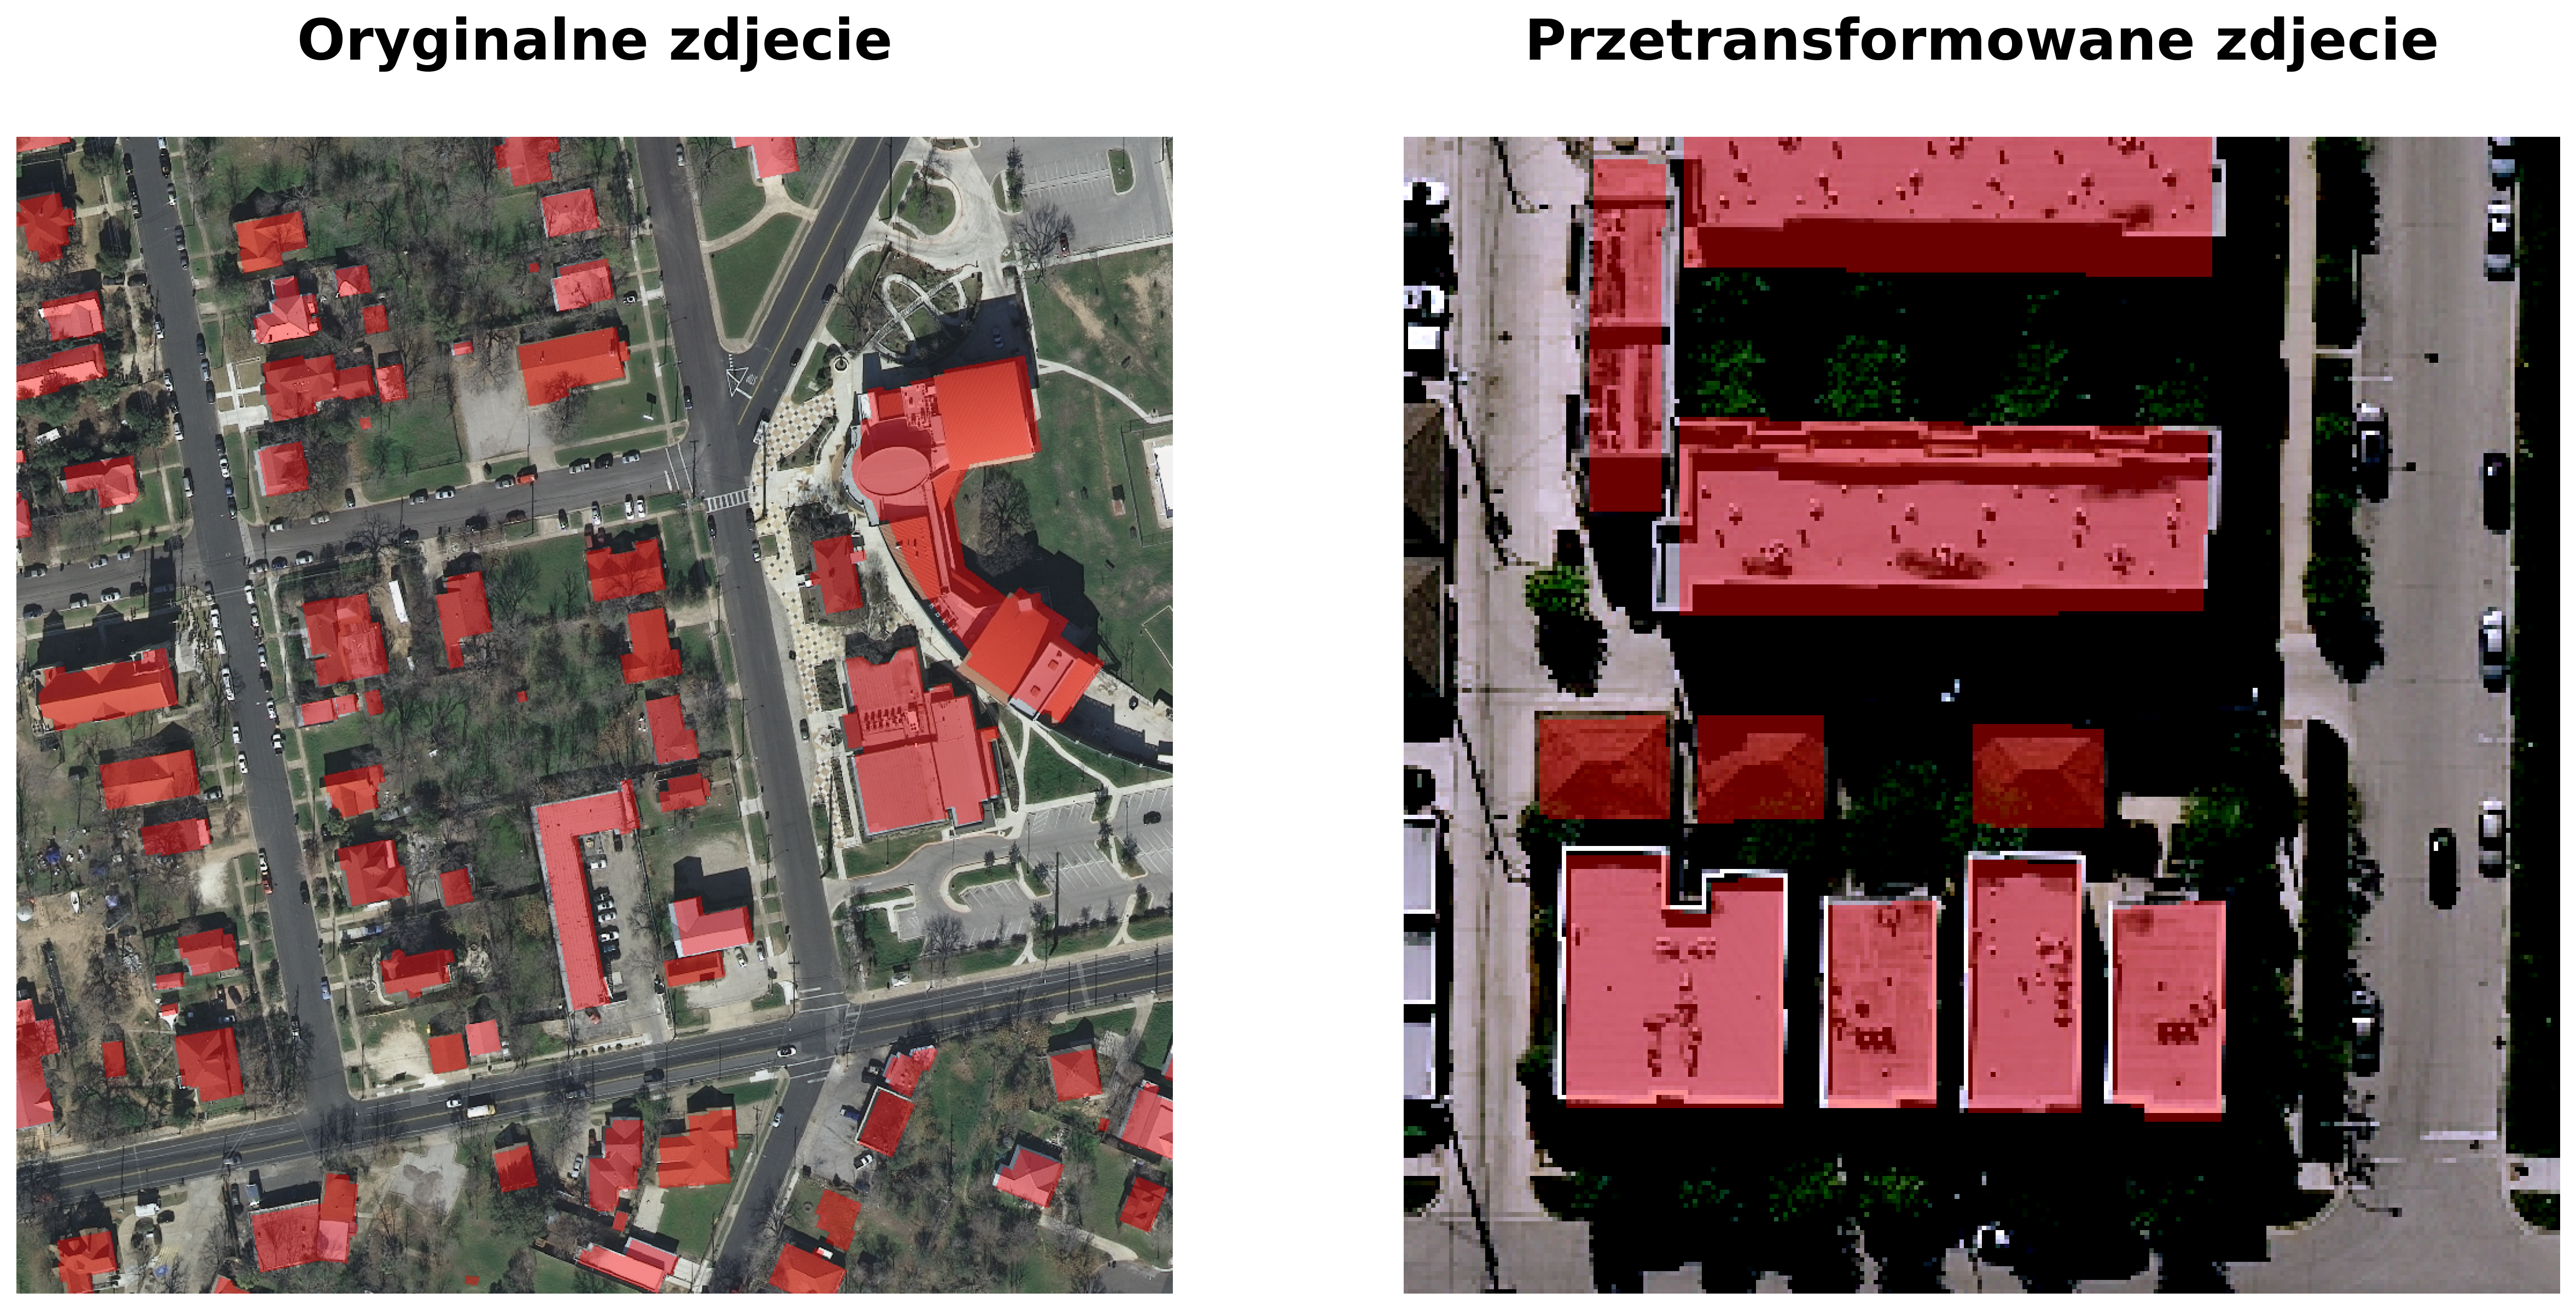
\includegraphics[width=1.0\linewidth]{Org_trans_img.png}
    \captionsetup{format=hang}
    \caption{Porównanie oryginalnego oraz przetransformowanego zdjęcia}
    \label{fig:org_trans1}
\end{figure}

\cell
Ostatnim etapem przygotowywania zbiorów treningowych i walidacyjnych było utworzenie dla nich obiektów ładujących dane (ang. data loader), które posłużyły bezpośrednio do zasilenia finalnego modelu w przykłady uczące / walidacyjne.

\cell
\begin{lstlisting}[name=Rozdzial3.1, language=Python]
train_data_gen = torch.utils.data.DataLoader(train_dataset, shuffle=True, 
                                             batch_size=batch_s, 
                                             num_workers=2, 
                                             pin_memory=True, 
                                             drop_last=True)

valid_data_gen = torch.utils.data.DataLoader(valid_dataset, 
                                             batch_size=batch_s, 
                                             num_workers=2, 
                                             pin_memory=True, 
                                             drop_last=True)

dataset_sizes = {'Train': len(train_data_gen.dataset), 'Valid': 
                 len(valid_data_gen.dataset)}

data_loaders = {'Train': train_data_gen, 'Valid': valid_data_gen}
\end{lstlisting}


\cell
Po ustrukturyzowaniu procesu wczytywania i obróbki danych, kolejnym krokiem  w budowie modelu detekcji budynków na zdjęciach lotniczych, była definicja finalnej architektury sieci $\textit{GML-Net}$.

\vspace{-0.5cm}
\cell
\ss{ Architektura sieci}

\cell
Architektura sieci $\textit{GML-Net}$ wzorowana jest na architekturze $\textit{U-Net}$, jest jednak od niej płytsza o jeden poziom ekstrakcji cech / upsamplingu, stąd też występują w niej tylko trzy połączenia rezydualne. Rolę enkodera w sieci $\textit{GML-Net}$ pełni sieć $\textit{Wide ResNet-50-2}$, która tym różni się od zwykłej sieci $\textit{ResNet-50}$, że posiada dwa razy więcej map cech w blokach rezydualnych, co czyni ją sporo szerszą i w efekcie skuteczniejszą w wychwytywaniu ukrytych zależności. Cechy wyekstraktowane przy pomocy $\textit{Wide ResNet-50-2}$ na danym poziomie rozdzielczości przestrzennej są następnie przetwarzane przez blok $\textit{BottleNeck}$ (wzorowany na blokach sieci $\textit{OSNet}$) po to by uzyskać zagregowany zbiór cech z przekroju różnych skal. Zbiór ten jest następnie transferowany, przy pomocy połączeń rezydualnych, bezpośrednio do warstw dekodera. Rekonstrukcja cech w dekoderze przeprowadzana jest przy pomocy konwolucji transponowanej. Zrekonstruowane cechy są przetwarzane przez blok $\textit{BottleNeck}$, a następnie przeprowadzana jest ich konkatenacja z cechami uzyskanymi z enkodera - tak połączone mapy cech stają się wsadem do kolejnych, wyższych warstw dekodera. W całej sieci powszechnie wykorzystywane są konwolucje separowalne wgłębnie i punktowo, co pozwala sieci $\textit{GML-Net}$ efektywnie nauczyć się korelacji kanałów przestrzennych, uniknąć nadmiernego dopasowania oraz uzyskać większą efektywność obliczeniową. Stąd też pomimo wykorzystania stosunkowo cieżkich architektur jakimi są bez wątpienia $\textit{U-Net}$ i $\textit{Wide ResNet-50-2}$, udało się ograniczyć liczbę trenowalnych parametrów finalnego modelu $\textit{GML-Net}$ do 27 milionów. Rysunek \ref{fig:gmlnet1} przedstawia architekturę omawianej w bieżącym rozdziale sieci:

\begin{figure}[!h]
    \centering \includegraphics[width=1.0\linewidth]{GML-Net.pdf}
    \captionsetup{format=hang}
    \caption{Architektura sieci \textit{GML-Net}}
    \label{fig:gmlnet1}
\end{figure}

Symbole nad poszczególnymi elementami sieci przedstawionej na powyższym rysunku zostały definiowane zgodnie z zapisem $\textit{STNN}$ dla architektur głębokich sieci neuronowych, który został opracowany przez prof. dr. hab. inż. Władysława Skarbka w artykule \textit{Symbolic Tensor Neural Networks for Digital Media – from Tensor Processing via BNF Graph Rules to CREAMS Applications} \cite{skarbek}. Poniżej zaprezentowano szczegółową definicję każdego z tych symboli:

\begin{equation*}
\begin{gathered}
\textbf{Ekstrakcja cech nr 1 - 64 mapy cech, rozdzielczość przestrzenna $\textit{128x128}$ ($\textit{ResNet64}$):}
\\~\\
\xunitdef{\boldsymbol{ResNet}}{\boldsymbol{128:\ 3\rightarrow64}}{\quad
\xinp{256_{xy}}{3}{}{}{}
\xconv{\ 7^k2^s}{\ 64}{p}{}{br}}
\end{gathered}
\end{equation*}
\begin{equation*}
\begin{gathered}
\textbf{Przetworzenie wyekstrahowanych cech $\textit{ResNet64}$ przez blok $\textit{DownBottleNeck64}$:}
\\~\\
\xunitdef{Btlnck64}{1}{\quad
\xunit{ResNet}{128:\ 3\rightarrow64}{} \quad
\xconv{\ 1^k1^s}{\ 16}{}{}{br}}
\\
\xunitdef{Btlnck64}{2}{\quad
\xconv{\ 1^k1^s}{\ 16}{}{}{}
\xconv{\ 3^k1^s}{\ 16}{p}{}{br}}
\\
\xunitdef{Btlnck64}{1-1}{\quad
\xunit{Btlnck64}{1}{} \quad
\xunit{Btlnck64}{2}{}}
\\
\xunitdef{Btlnck64}{1-2}{\quad
\xaggreg{\quad
\xunit{Btlnck64}{1-1}{}
\quad \left|_{\bigotimes} \quad
\xunit{Btlnck64}{1-1}{}
\xpool{g}{}{a}{}{}
\xconv{\ 1^k1^s}{\ 16}{}{}{r}
\xconv{\ 1^k1^s}{\ 16}{}{}{s}
\right.}}
\\
\xunitdef{Btlnck64}{2-1}{\quad
\xunit{Btlnck64}{1-1}{} \quad
\xunit{Btlnck64}{2}{}}
\\
\xunitdef{Btlnck64}{2-2}{\quad
\xaggreg{\quad
\xunit{Btlnck64}{2-1}{}
\quad \left|_{\bigotimes} \quad
\xunit{Btlnck64}{2-1}{}
\xpool{g}{}{a}{}{}
\xconv{\ 1^k1^s}{\ 16}{}{}{r}
\xconv{\ 1^k1^s}{\ 16}{}{}{s}
\right.}}
\\
\xunitdef{Btlnck64}{3-1}{\quad
\xunit{Btlnck64}{2-1}{} \quad
\xunit{Btlnck64}{2}{}}
\\
\xunitdef{Btlnck64}{3-2}{\quad
\xaggreg{\quad
\xunit{Btlnck64}{3-1}{}
\quad \left|_{\bigotimes} \quad
\xunit{Btlnck64}{3-1}{}
\xpool{g}{}{a}{}{}
\xconv{\ 1^k1^s}{\ 16}{}{}{r}
\xconv{\ 1^k1^s}{\ 16}{}{}{s}
\right.}}
\\
\xunitdef{Btlnck64}{4-1}{\quad
\xunit{Btlnck64}{3-1}{} \quad
\xunit{Btlnck64}{2}{}}
\\
\xunitdef{Btlnck64}{4-2}{\quad
\xaggreg{\quad
\xunit{Btlnck64}{4-1}{}
\quad \left|_{\bigotimes} \quad
\xunit{Btlnck64}{4-1}{}
\xpool{g}{}{a}{}{}
\xconv{\ 1^k1^s}{\ 16}{}{}{r}
\xconv{\ 1^k1^s}{\ 16}{}{}{s}
\right.}}
\\
\xunitdef{Btlnck64}{5}{\quad
\xaggreg{\quad
\xaggreg{\quad
\xaggreg{\quad
\xunit{Btlnck64}{1-2}{}
\quad \left|_+ \quad
\xunit{Btlnck64}{2-2}{}
\right.\quad}
\quad \left|_+ \quad
\xunit{Btlnck64}{3-2}{}
\right.\quad}
\quad \left|_+ \quad
\xunit{Btlnck64}{4-2}{}
\right.\quad}}
\\
\xunitdef{\boldsymbol{DownBottleNeck}}{\boldsymbol{128:\ 64\rightarrow64}}{\quad
\xaggreg{\quad
\xunit{ResNet}{128:\ 3\rightarrow64}{}
\quad \left|_+ \quad
\xunit{Btlnck64}{5}{}
\xconv{\ 1^k1^s}{\ 64}{}{}{b}
\right.}^r}
\end{gathered}
\end{equation*}
\begin{equation*}
\begin{gathered}
\textbf{Ekstrakcja cech nr 2 - 256 map cech, rozdzielczość przestrzenna $\textit{64x64}$ ($\textit{ResNet256}$):}
\\~\\
\xunitdef{resnet256}{1}{
\xaggreg{\quad
\xunit{ResNet}{128:\ 3\rightarrow64}{}
\xpool{3^k2^s}{}{mp}{}{}
\xconv{\ 1^k1^s}{\ 128}{}{}{br}
\xconv{\ 3^k1^s}{\ 128}{p}{}{br}
\xconv{\ 1^k1^s}{\ 256}{}{}{b}
\quad \left|_+ \quad
\xunit{ResNet}{128:\ 3\rightarrow64}{}
\xpool{3^k2^s}{}{mp}{}{}
\xconv{\ 1^k1^s}{\ 256}{}{}{b}
\right.}^r}
\\
\xunitdef{resnet256}{2}{
\xaggreg{\quad
\xunit{resnet256}{1}{}
\quad \left|_+ \quad
\xunit{resnet256}{1}{}
\xconv{\ 1^k1^s}{\ 128}{}{}{br}
\xconv{\ 3^k1^s}{\ 128}{p}{}{br}
\xconv{\ 1^k1^s}{\ 256}{}{}{b}
\right.}^r}
\\
\xunitdef{resnet256}{3}{
\xaggreg{\quad
\xunit{resnet256}{2}{}
\quad \left|_+ \quad
\xunit{resnet256}{2}{}
\xconv{\ 1^k1^s}{\ 128}{}{}{br}
\xconv{\ 3^k1^s}{\ 128}{p}{}{br}
\xconv{\ 1^k1^s}{\ 256}{}{}{b}
\right.}^r}
\\
\xunitdef{\boldsymbol{ResNet}}{\boldsymbol{64:\ 64\rightarrow256}}{ \quad
\xunit{resnet256}{1}{} \quad
\xunit{resnet256}{2}{} \quad
\xunit{resnet256}{3}{}}
\end{gathered}
\end{equation*}
\begin{equation*}
\begin{gathered}
\textbf{Przetworzenie wyekstrahowanych cech $\textit{ResNet256}$ przez blok $\textit{DownBottleNeck128}$:}
\\~\\
\xunitdef{Btlnck256}{1}{\quad
\xunit{ResNet}{64\rightarrow256}{} \quad
\xconv{\ 1^k1^s}{\ 32}{}{}{br}}
\\
\xunitdef{Btlnck256}{2}{\quad
\xconv{\ 1^k1^s}{\ 32}{}{}{}
\xconv{\ 3^k1^s}{\ 32}{p}{}{br}}
\\
\xunitdef{Btlnck256}{1-1}{\quad
\xunit{Btlnck256}{1}{} \quad
\xunit{Btlnck256}{2}{}}
\\
\xunitdef{Btlnck256}{1-2}{\quad
\xaggreg{\quad
\xunit{Btlnck256}{1-1}{}
\quad \left|_{\bigotimes} \quad
\xunit{Btlnck256}{1-1}{}
\xpool{g}{}{a}{}{}
\xconv{\ 1^k1^s}{\ 32}{}{}{r}
\xconv{\ 1^k1^s}{\ 32}{}{}{s}
\right.}}
\\
\xunitdef{Btlnck256}{2-1}{\quad
\xunit{Btlnck256}{1-1}{} \quad
\xunit{Btlnck256}{2}{}}
\\
\xunitdef{Btlnck256}{2-2}{\quad
\xaggreg{\quad
\xunit{Btlnck256}{2-1}{}
\quad \left|_{\bigotimes} \quad
\xunit{Btlnck256}{2-1}{}
\xpool{g}{}{a}{}{}
\xconv{\ 1^k1^s}{\ 32}{}{}{r}
\xconv{\ 1^k1^s}{\ 32}{}{}{s}
\right.}}
\\
\xunitdef{Btlnck256}{3-1}{\quad
\xunit{Btlnck256}{2-1}{} \quad
\xunit{Btlnck256}{2}{}}
\\
\xunitdef{Btlnck256}{3-2}{\quad
\xaggreg{\quad
\xunit{Btlnck256}{3-1}{}
\quad \left|_{\bigotimes} \quad
\xunit{Btlnck256}{3-1}{}
\xpool{g}{}{a}{}{}
\xconv{\ 1^k1^s}{\ 32}{}{}{r}
\xconv{\ 1^k1^s}{\ 32}{}{}{s}
\right.}}
\end{gathered}
\end{equation*}
\begin{equation*}
\begin{gathered}
\xunitdef{Btlnck256}{4-1}{\quad
\xunit{Btlnck256}{3-1}{} \quad
\xunit{Btlnck256}{2}{}}
\\
\xunitdef{Btlnck256}{4-2}{\quad
\xaggreg{\quad
\xunit{Btlnck256}{4-1}{}
\quad \left|_{\bigotimes} \quad
\xunit{Btlnck256}{4-1}{}
\xpool{g}{}{a}{}{}
\xconv{\ 1^k1^s}{\ 32}{}{}{r}
\xconv{\ 1^k1^s}{\ 32}{}{}{s}
\right.}}
\\
\xunitdef{Btlnck256}{5}{\quad
\xaggreg{\quad
\xaggreg{\quad
\xaggreg{\quad
\xunit{Btlnck256}{1-2}{}
\quad \left|_+ \quad
\xunit{Btlnck256}{2-2}{}
\right.\quad}
\quad \left|_+ \quad
\xunit{Btlnck256}{3-2}{}
\right.\quad}
\quad \left|_+ \quad
\xunit{Btlnck256}{4-2}{}
\right.\quad}}
\\
\xunitdef{\boldsymbol{DownBottleNeck}}{\boldsymbol{64:\ 256\rightarrow128}}{\quad
\xaggreg{\quad
\xunit{ResNet}{64\rightarrow256}{}
\xconv{\ 1^k1^s}{\ 128}{}{}{b}
\quad \left|_+ \quad
\xunit{Btlnck256}{5}{}
\xconv{\ 1^k1^s}{\ 128}{}{}{b}
\right.}^r}
\end{gathered}
\end{equation*}
\begin{equation*}
\begin{gathered}
\textbf{Ekstrakcja cech nr 3 - 512 map cech, rozdzielczość przestrzenna $\textit{32x32}$ ($\textit{ResNet512}$):}
\\~\\
\xunitdef{resnet512}{1}{
\xaggreg{\quad
\xunit{ResNet}{64\rightarrow256}{}
\xconv{\ 1^k1^s}{\ 256}{}{}{br}
\xconv{\ 3^k2^s}{\ 256}{p}{}{br}
\xconv{\ 1^k1^s}{\ 512}{}{}{b}
\quad \left|_+ \quad
\xunit{ResNet}{64\rightarrow256}{}
\xconv{\ 1^k2^s}{\ 512}{}{}{b}
\right.}^r}
\\
\xunitdef{resnet512}{2}{
\xaggreg{\quad
\xunit{resnet512}{1}{}
\quad \left|_+ \quad
\xunit{resnet512}{1}{}
\xconv{\ 1^k1^s}{\ 256}{}{}{br}
\xconv{\ 3^k1^s}{\ 256}{p}{}{br}
\xconv{\ 1^k1^s}{\ 512}{}{}{b}
\right.}^r}
\\
\xunitdef{resnet512}{3}{
\xaggreg{\quad
\xunit{resnet512}{2}{}
\quad \left|_+ \quad
\xunit{resnet512}{2}{}
\xconv{\ 1^k1^s}{\ 256}{}{}{br}
\xconv{\ 3^k1^s}{\ 256}{p}{}{br}
\xconv{\ 1^k1^s}{\ 512}{}{}{b}
\right.}^r}
\\
\xunitdef{resnet512}{4}{
\xaggreg{\quad
\xunit{resnet512}{3}{}
\quad \left|_+ \quad
\xunit{resnet512}{3}{}
\xconv{\ 1^k1^s}{\ 256}{}{}{br}
\xconv{\ 3^k1^s}{\ 256}{p}{}{br}
\xconv{\ 1^k1^s}{\ 512}{}{}{b}
\right.}^r}
\\
\xunitdef{\boldsymbol{ResNet}}{\boldsymbol{32:\ 256\rightarrow512}}{ \quad
\xunit{resnet512}{1}{} \quad
\xunit{resnet512}{2}{} \quad
\xunit{resnet512}{3}{} \quad
\xunit{resnet512}{4}{}}
\end{gathered}
\end{equation*}
\begin{equation*}
\begin{gathered}
\textbf{Przetworzenie wyekstrahowanych cech $\textit{ResNet512}$ przez blok $\textit{DownBottleNeck256}$:}
\\~\\
\xunitdef{Btlnck512}{1}{\quad
\xunit{ResNet}{32:\ 256\rightarrow512}{} \quad
\xconv{\ 1^k1^s}{\ 64}{}{}{br}}
\\
\xunitdef{Btlnck512}{2}{\quad
\xconv{\ 1^k1^s}{\ 64}{}{}{}
\xconv{\ 3^k1^s}{\ 64}{p}{}{br}}
\\
\xunitdef{Btlnck512}{1-1}{\quad
\xunit{Btlnck512}{1}{} \quad
\xunit{Btlnck512}{2}{}}
\end{gathered}
\end{equation*}
\begin{equation*}
\begin{gathered}
\xunitdef{Btlnck512}{1-2}{\quad
\xaggreg{\quad
\xunit{Btlnck512}{1-1}{}
\quad \left|_{\bigotimes} \quad
\xunit{Btlnck512}{1-1}{}
\xpool{g}{}{a}{}{}
\xconv{\ 1^k1^s}{\ 64}{}{}{r}
\xconv{\ 1^k1^s}{\ 64}{}{}{s}
\right.}}
\\
\xunitdef{Btlnck512}{2-1}{\quad
\xunit{Btlnck512}{1-1}{} \quad
\xunit{Btlnck512}{2}{}}
\\
\xunitdef{Btlnck512}{2-2}{\quad
\xaggreg{\quad
\xunit{Btlnck512}{2-1}{}
\quad \left|_{\bigotimes} \quad
\xunit{Btlnck512}{2-1}{}
\xpool{g}{}{a}{}{}
\xconv{\ 1^k1^s}{\ 64}{}{}{r}
\xconv{\ 1^k1^s}{\ 64}{}{}{s}
\right.}}
\\
\xunitdef{Btlnck512}{3-1}{\quad
\xunit{Btlnck512}{2-1}{} \quad
\xunit{Btlnck512}{2}{}}
\\
\xunitdef{Btlnck512}{3-2}{\quad
\xaggreg{\quad
\xunit{Btlnck512}{3-1}{}
\quad \left|_{\bigotimes} \quad
\xunit{Btlnck512}{3-1}{}
\xpool{g}{}{a}{}{}
\xconv{\ 1^k1^s}{\ 64}{}{}{r}
\xconv{\ 1^k1^s}{\ 64}{}{}{s}
\right.}}
\\
\xunitdef{Btlnck512}{4-1}{\quad
\xunit{Btlnck512}{3-1}{} \quad
\xunit{Btlnck512}{2}{}}
\\
\xunitdef{Btlnck512}{4-2}{\quad
\xaggreg{\quad
\xunit{Btlnck512}{4-1}{}
\quad \left|_{\bigotimes} \quad
\xunit{Btlnck512}{4-1}{}
\xpool{g}{}{a}{}{}
\xconv{\ 1^k1^s}{\ 64}{}{}{r}
\xconv{\ 1^k1^s}{\ 64}{}{}{s}
\right.}}
\\
\xunitdef{Btlnck512}{5}{\quad
\xaggreg{\quad
\xaggreg{\quad
\xaggreg{\quad
\xunit{Btlnck512}{1-2}{}
\quad \left|_+ \quad
\xunit{Btlnck512}{2-2}{}
\right.\quad}
\quad \left|_+ \quad
\xunit{Btlnck512}{3-2}{}
\right.\quad}
\quad \left|_+ \quad
\xunit{Btlnck512}{4-2}{}
\right.\quad}}
\\
\xunitdef{\boldsymbol{DownBottleNeck}}{\boldsymbol{32:\ 512\rightarrow256}}{\quad
\xaggreg{\quad
\xunit{ResNet}{32:\ 256\rightarrow512}{}
\xconv{\ 1^k1^s}{\ 256}{}{}{b}
\quad \left|_+ \quad
\xunit{Btlnck512}{5}{}
\xconv{\ 1^k1^s}{\ 256}{}{}{b}
\right.}^r}
\end{gathered}
\end{equation*}
\begin{equation*}
\begin{gathered}
\textbf{Ekstrakcja cech nr 4 - 1024 mapy cech, rozdzielczość przestrzenna $\textit{16x16}$ ($\textit{ResNet1024}$):}
\\~\\
\xunitdef{resnet1024}{1}{
\xaggreg{\quad
\xunit{ResNet}{32:\ 256-512}{}
\xconv{\ 1^k1^s}{\ 512}{}{}{br}
\xconv{\ 3^k2^s}{\ 512}{p}{}{br}
\xconv{\ 1^k1^s}{\ 1024}{}{}{b}
\quad \left|_+ \quad
\xunit{ResNet}{32:\ 256-512}{}
\xconv{\ 1^k2^s}{\ 1024}{}{}{b}
\right.}^r}
\\
\xunitdef{resnet1024}{2}{
\xaggreg{\quad
\xunit{resnet1024}{1}{}
\quad \left|_+ \quad
\xunit{resnet1024}{1}{}
\xconv{\ 1^k1^s}{\ 512}{}{}{br}
\xconv{\ 3^k1^s}{\ 512}{p}{}{br}
\xconv{\ 1^k1^s}{\ 1024}{}{}{b}
\right.}^r}
\\
\xunitdef{resnet1024}{3}{
\xaggreg{\quad
\xunit{resnet1024}{2}{}
\quad \left|_+ \quad
\xunit{resnet1024}{2}{}
\xconv{\ 1^k1^s}{\ 512}{}{}{br}
\xconv{\ 3^k1^s}{\ 512}{p}{}{br}
\xconv{\ 1^k1^s}{\ 1024}{}{}{b}
\right.}^r}
\\
\xunitdef{resnet1024}{4}{
\xaggreg{\quad
\xunit{resnet1024}{3}{}
\quad \left|_+ \quad
\xunit{resnet1024}{3}{}
\xconv{\ 1^k1^s}{\ 512}{}{}{br}
\xconv{\ 3^k1^s}{\ 512}{p}{}{br}
\xconv{\ 1^k1^s}{\ 1024}{}{}{b}
\right.}^r}
\end{gathered}
\end{equation*}
\begin{equation*}
\begin{gathered}
\xunitdef{resnet1024}{5}{
\xaggreg{\quad
\xunit{resnet1024}{4}{}
\quad \left|_+ \quad
\xunit{resnet1024}{4}{}
\xconv{\ 1^k1^s}{\ 512}{}{}{br}
\xconv{\ 3^k1^s}{\ 512}{p}{}{br}
\xconv{\ 1^k1^s}{\ 1024}{}{}{b}
\right.}^r}
\\
\xunitdef{resnet1024}{6}{
\xaggreg{\quad
\xunit{resnet1024}{5}{}
\quad \left|_+ \quad
\xunit{resnet1024}{5}{}
\xconv{\ 1^k1^s}{\ 512}{}{}{br}
\xconv{\ 3^k1^s}{\ 512}{p}{}{br}
\xconv{\ 1^k1^s}{\ 1024}{}{}{b}
\right.}^r}
\\
\xunitdef{\boldsymbol{ResNet}}{\boldsymbol{16:\ 512-1024}}{ \quad
\xunit{resnet1024}{1}{} \quad
\xunit{resnet1024}{2}{} \quad
\xunit{resnet1024}{3}{} \quad
\xunit{resnet1024}{4}{} \quad
\xunit{resnet1024}{5}{}\quad
\xunit{resnet1024}{6}{}}
\end{gathered}
\end{equation*}
\begin{equation*}
\begin{gathered}
\textbf{Przetworzenie wyekstrahowanych cech $\textit{ResNet1024}$ przez blok $\textit{DownBottleNeck512}$:}
\\~\\
\xunitdef{Btlnck1024}{1}{\quad
\xunit{ResNet}{16:\ 512\rightarrow1024}{} \quad
\xconv{\ 1^k1^s}{\ 128}{}{}{br}}
\\
\xunitdef{Btlnck1024}{2}{\quad
\xconv{\ 1^k1^s}{\ 128}{}{}{}
\xconv{\ 3^k1^s}{\ 128}{p}{}{br}}
\\
\xunitdef{Btlnck1024}{1-1}{\quad
\xunit{Btlnck1024}{1}{} \quad
\xunit{Btlnck1024}{2}{}}
\\
\xunitdef{Btlnck1024}{1-2}{\quad
\xaggreg{\quad
\xunit{Btlnck1024}{1-1}{}
\quad \left|_{\bigotimes} \quad
\xunit{Btlnck1024}{1-1}{}
\xpool{g}{}{a}{}{}
\xconv{\ 1^k1^s}{\ 128}{}{}{r}
\xconv{\ 1^k1^s}{\ 128}{}{}{s}
\right.}}
\\
\xunitdef{Btlnck1024}{2-1}{\quad
\xunit{Btlnck1024}{1-1}{} \quad
\xunit{Btlnck1024}{2}{}}
\\
\xunitdef{Btlnck1024}{2-2}{\quad
\xaggreg{\quad
\xunit{Btlnck1024}{2-1}{}
\quad \left|_{\bigotimes} \quad
\xunit{Btlnck1024}{2-1}{}
\xpool{g}{}{a}{}{}
\xconv{\ 1^k1^s}{\ 128}{}{}{r}
\xconv{\ 1^k1^s}{\ 128}{}{}{s}
\right.}}
\\
\xunitdef{Btlnck1024}{3-1}{\quad
\xunit{Btlnck1024}{2-1}{} \quad
\xunit{Btlnck1024}{2}{}}
\\
\xunitdef{Btlnck1024}{3-2}{\quad
\xaggreg{\quad
\xunit{Btlnck1024}{3-1}{}
\quad \left|_{\bigotimes} \quad
\xunit{Btlnck1024}{3-1}{}
\xpool{g}{}{a}{}{}
\xconv{\ 1^k1^s}{\ 128}{}{}{r}
\xconv{\ 1^k1^s}{\ 128}{}{}{s}
\right.}}
\\
\xunitdef{Btlnck1024}{4-1}{\quad
\xunit{Btlnck1024}{3-1}{} \quad
\xunit{Btlnck1024}{2}{}}
\\
\xunitdef{Btlnck1024}{4-2}{\quad
\xaggreg{\quad
\xunit{Btlnck1024}{4-1}{}
\quad \left|_{\bigotimes} \quad
\xunit{Btlnck1024}{4-1}{}
\xpool{g}{}{a}{}{}
\xconv{\ 1^k1^s}{\ 128}{}{}{r}
\xconv{\ 1^k1^s}{\ 128}{}{}{s}
\right.}}
\\
\xunitdef{Btlnck1024}{5}{\quad
\xaggreg{\quad
\xaggreg{\quad
\xaggreg{\quad
\xunit{Btlnck1024}{1-2}{}
\quad \left|_+ \quad
\xunit{Btlnck1024}{2-2}{}
\right.\quad}
\quad \left|_+ \quad
\xunit{Btlnck1024}{3-2}{}
\right.\quad}
\quad \left|_+ \quad
\xunit{Btlnck1024}{4-2}{}
\right.\quad}}
\end{gathered}
\end{equation*}
\begin{equation*}
\begin{gathered}
\xunitdef{\boldsymbol{DownBottleNeck}}{\boldsymbol{16:\ 1024\rightarrow512}}{\quad
\xaggreg{\quad
\xunit{ResNet}{16:\ 512\rightarrow1024}{}
\xconv{\ 1^k1^s}{\ 512}{}{}{b}
\quad \left|_+ \quad
\xunit{Btlnck1024}{5}{}
\xconv{\ 1^k1^s}{\ 512}{}{}{b}
\right.}^r}
\end{gathered}
\end{equation*}
\begin{equation*}
\begin{gathered}
\textbf{Rekonstrukcja nr 1 - 256 map cech, rozdzielczość przestrzenna $\textit{32x32}$ ($\textit{TransConv256}$):}
\\~\\
\xunitdef{\boldsymbol{TransConv}}{\boldsymbol{32:\ 512\rightarrow256}}{\quad
\xunit{DownBottleNeck}{16:\ 1024\rightarrow512}{}
\xconv{\ 1^k1^s}{\ 256}{}{}{}
\xconv{\ 1^k1^s}{\ 256}{}{}{r}
\xconv{\ 2^k2^s}{\ 256}{t}{}{}}
\end{gathered}
\end{equation*}
\begin{equation*}
\begin{gathered}
\textbf{Przetworzenie nadpróbkowanych cech $\textit{TransConv256}$ przez blok $\textit{UpBottleNeck192}$:}
\\~\\
\xunitdef{UpBtnk256}{1}{\quad
\xunit{TransConv}{32:\ 512\rightarrow256}{} \quad
\xconv{\ 1^k1^s}{\ 48}{}{}{br}}
\\
\xunitdef{UpBtnk256}{2}{\quad
\xconv{\ 1^k1^s}{\ 48}{}{}{}
\xconv{\ 3^k1^s}{\ 48}{p}{}{br}}
\\
\xunitdef{UpBtnk256}{1-1}{\quad
\xunit{UpBtnk256}{1}{} \quad
\xunit{UpBtnk256}{2}{}}
\\
\xunitdef{UpBtnk256}{1-2}{\quad
\xaggreg{\quad
\xunit{UpBtnk256}{1-1}{}
\quad \left|_{\bigotimes} \quad
\xunit{UpBtnk256}{1-1}{}
\xpool{g}{}{a}{}{}
\xconv{\ 1^k1^s}{\ 48}{}{}{r}
\xconv{\ 1^k1^s}{\ 48}{}{}{s}
\right.}}
\\
\xunitdef{UpBtnk256}{2-1}{\quad
\xunit{UpBtnk256}{1-1}{} \quad
\xunit{UpBtnk256}{2}{}}
\\
\xunitdef{UpBtnk256}{2-2}{\quad
\xaggreg{\quad
\xunit{UpBtnk256}{2-1}{}
\quad \left|_{\bigotimes} \quad
\xunit{UpBtnk256}{2-1}{}
\xpool{g}{}{a}{}{}
\xconv{\ 1^k1^s}{\ 48}{}{}{r}
\xconv{\ 1^k1^s}{\ 48}{}{}{s}
\right.}}
\\
\xunitdef{UpBtnk256}{3-1}{\quad
\xunit{UpBtnk256}{2-1}{} \quad
\xunit{UpBtnk256}{2}{}}
\\
\xunitdef{UpBtnk256}{3-2}{\quad
\xaggreg{\quad
\xunit{UpBtnk256}{3-1}{}
\quad \left|_{\bigotimes} \quad
\xunit{UpBtnk256}{3-1}{}
\xpool{g}{}{a}{}{}
\xconv{\ 1^k1^s}{\ 48}{}{}{r}
\xconv{\ 1^k1^s}{\ 48}{}{}{s}
\right.}}
\\
\xunitdef{UpBtnk256}{4-1}{\quad
\xunit{UpBtnk256}{3-1}{} \quad
\xunit{UpBtnk256}{2}{}}
\\
\xunitdef{UpBtnk256}{4-2}{\quad
\xaggreg{\quad
\xunit{UpBtnk256}{4-1}{}
\quad \left|_{\bigotimes} \quad
\xunit{UpBtnk256}{4-1}{}
\xpool{g}{}{a}{}{}
\xconv{\ 1^k1^s}{\ 48}{}{}{r}
\xconv{\ 1^k1^s}{\ 48}{}{}{s}
\right.}}
\end{gathered}
\end{equation*}
\begin{equation*}
\begin{gathered}
\xunitdef{UpBtnk256}{5}{\quad
\xaggreg{\quad
\xaggreg{\quad
\xaggreg{\quad
\xunit{UpBtnk256}{1-2}{}
\quad \left|_+ \quad
\xunit{UpBtnk256}{2-2}{}
\right.\quad}
\quad \left|_+ \quad
\xunit{UpBtnk256}{3-2}{}
\right.\quad}
\quad \left|_+ \quad
\xunit{UpBtnk256}{4-2}{}
\right.\quad}}
\\
\xunitdef{\boldsymbol{UpBottleNeck}}{\boldsymbol{32:\ 256\rightarrow192}}{\quad
\xaggreg{\quad
\xunit{TransConv}{32:\ 512\rightarrow256}{}
\xconv{\ 1^k1^s}{\ 192}{}{}{b}
\quad \left|_+ \quad
\xunit{UpBtnk256}{5}{}
\xconv{\ 1^k1^s}{\ 192}{}{}{b}
\right.}^r}
\end{gathered}
\end{equation*}
\begin{equation*}
\begin{gathered}
\textbf{Konkatenacja nr 1 - 448 map cech, rozdzielczość przestrzenna $\textit{32x32}$ ($\textit{ConCat448}$):}
\\~\\
\xunitdef{\boldsymbol{ConCat}}{\boldsymbol{32:\ \langle \; 256 \; | \; 192 \; \rangle}}{\quad
\xaggreg{\quad
\xunit{UpBottleNeck}{32:\ 256\rightarrow192}{}
\quad \left| \quad
\xunit{DownBottleNeck}{32:\ 512\rightarrow256}{}
\right.}}
\end{gathered}
\end{equation*}
\begin{equation*}
\begin{gathered}
\textbf{Rekonstrukcja nr 2 - 192 mapy cech, rozdzielczość przestrzenna $\textit{64x64}$ ($\textit{TransConv192}$):}
\\~\\
\xunitdef{\boldsymbol{TransConv}}{\boldsymbol{64:\ 448\rightarrow192}}{\quad
\xunit{ConCat}{32:\ \langle \; 256 \; | \; 192 \; \rangle}{}
\xconv{\ 1^k1^s}{\ 192}{}{}{}
\xconv{\ 3^k1^s}{\ 192}{p}{}{br}
\xconv{\ 2^k2^s}{\ 192}{t}{}{}}
\end{gathered}
\end{equation*}
\begin{equation*}
\begin{gathered}
\textbf{Przetworzenie nadpróbkowanych cech $\textit{TransConv192}$ przez blok $\textit{UpBottleNeck128}$:}
\\~\\
\xunitdef{UpBtnk128}{1}{\quad
\xunit{TransConv}{64:\ 448\rightarrow192}{} \quad
\xconv{\ 1^k1^s}{\ 32}{}{}{br}}
\\
\xunitdef{UpBtnk128}{2}{\quad
\xconv{\ 1^k1^s}{\ 32}{}{}{}
\xconv{\ 3^k1^s}{\ 32}{p}{}{br}}
\\
\xunitdef{UpBtnk128}{1-1}{\quad
\xunit{UpBtnk128}{1}{} \quad
\xunit{UpBtnk128}{2}{}}
\\
\xunitdef{UpBtnk128}{1-2}{\quad
\xaggreg{\quad
\xunit{UpBtnk128}{1-1}{}
\quad \left|_{\bigotimes} \quad
\xunit{UpBtnk128}{1-1}{}
\xpool{g}{}{a}{}{}
\xconv{\ 1^k1^s}{\ 32}{}{}{r}
\xconv{\ 1^k1^s}{\ 32}{}{}{s}
\right.}}
\\
\xunitdef{UpBtnk128}{2-1}{\quad
\xunit{UpBtnk128}{1-1}{} \quad
\xunit{UpBtnk128}{2}{}}
\\
\xunitdef{UpBtnk128}{2-2}{\quad
\xaggreg{\quad
\xunit{UpBtnk128}{2-1}{}
\quad \left|_{\bigotimes} \quad
\xunit{UpBtnk128}{2-1}{}
\xpool{g}{}{a}{}{}
\xconv{\ 1^k1^s}{\ 32}{}{}{r}
\xconv{\ 1^k1^s}{\ 32}{}{}{s}
\right.}}
\end{gathered}
\end{equation*}
\begin{equation*}
\begin{gathered}
\xunitdef{UpBtnk128}{3-1}{\quad
\xunit{UpBtnk128}{2-1}{} \quad
\xunit{UpBtnk128}{2}{}}
\\
\xunitdef{UpBtnk128}{3-2}{\quad
\xaggreg{\quad
\xunit{UpBtnk128}{3-1}{}
\quad \left|_{\bigotimes} \quad
\xunit{UpBtnk128}{3-1}{}
\xpool{g}{}{a}{}{}
\xconv{\ 1^k1^s}{\ 32}{}{}{r}
\xconv{\ 1^k1^s}{\ 32}{}{}{s}
\right.}}
\\
\xunitdef{UpBtnk128}{4-1}{\quad
\xunit{UpBtnk128}{3-1}{} \quad
\xunit{UpBtnk128}{2}{}}
\\
\xunitdef{UpBtnk128}{4-2}{\quad
\xaggreg{\quad
\xunit{UpBtnk128}{4-1}{}
\quad \left|_{\bigotimes} \quad
\xunit{UpBtnk128}{4-1}{}
\xpool{g}{}{a}{}{}
\xconv{\ 1^k1^s}{\ 32}{}{}{r}
\xconv{\ 1^k1^s}{\ 32}{}{}{s}
\right.}}
\\
\xunitdef{UpBtnk128}{5}{\quad
\xaggreg{\quad
\xaggreg{\quad
\xaggreg{\quad
\xunit{UpBtnk128}{1-2}{}
\quad \left|_+ \quad
\xunit{UpBtnk128}{2-2}{}
\right.\quad}
\quad \left|_+ \quad
\xunit{UpBtnk128}{3-2}{}
\right.\quad}
\quad \left|_+ \quad
\xunit{UpBtnk128}{4-2}{}
\right.\quad}}
\\
\xunitdef{\boldsymbol{UpBottleNeck}}{\boldsymbol{64:\ 192\rightarrow128}}{\quad
\xaggreg{\quad
\xunit{TransConv}{64:\ 448\rightarrow192}{}
\xconv{\ 1^k1^s}{\ 128}{}{}{b}
\quad \left|_+ \quad
\xunit{UpBtnk128}{5}{}
\xconv{\ 1^k1^s}{\ 128}{}{}{b}
\right.}^r}
\end{gathered}
\end{equation*}
\begin{equation*}
\begin{gathered}
\textbf{Konkatenacja nr 2 - 256 map cech, rozdzielczość przestrzenna $\textit{64x64}$ ($\textit{ConCat256}$):}
\\~\\
\xunitdef{\boldsymbol{ConCat}}{\boldsymbol{64:\ \langle \; 128 \; | \; 128 \; \rangle}}{\quad
\xaggreg{\quad
\xunit{UpBottleNeck}{64:\ 192\rightarrow128}{}
\quad \left| \quad
\xunit{DownBottleNeck}{64:\ 256\rightarrow128}{}
\right.}}
\end{gathered}
\end{equation*}
\begin{equation*}
\begin{gathered}
\textbf{Rekonstrukcja nr 3 - 128 map cech, rozdzielczość przestrzenna $\textit{128x128}$ ($\textit{TransConv128}$):}
\\~\\
\xunitdef{\boldsymbol{TransConv}}{\boldsymbol{128:\ 256\rightarrow128}}{\quad
\xunit{ConCat}{64:\ \langle \; 128 \; | \; 128 \; \rangle}{}
\xconv{\ 1^k1^s}{\ 128}{}{}{}
\xconv{\ 3^k1^s}{\ 128}{p}{}{br}
\xconv{\ 2^k2^s}{\ 128}{t}{}{}}
\end{gathered}
\end{equation*}
\begin{equation*}
\begin{gathered}
\textbf{Przetworzenie nadpróbkowanych cech $\textit{TransConv128}$ przez blok $\textit{UpBottleNeck64}$:}
\\~\\
\xunitdef{UpBtnk64}{1}{\quad
\xunit{TransConv}{128:\ 256\rightarrow128}{} \quad
\xconv{\ 1^k1^s}{\ 16}{}{}{br}}
\\
\xunitdef{UpBtnk64}{2}{\quad
\xconv{\ 1^k1^s}{\ 16}{}{}{}
\xconv{\ 3^k1^s}{\ 16}{p}{}{br}}
\end{gathered}
\end{equation*}
\begin{equation*}
\begin{gathered}
\xunitdef{UpBtnk64}{1-1}{\quad
\xunit{UpBtnk64}{1}{} \quad
\xunit{UpBtnk64}{2}{}}
\\
\xunitdef{UpBtnk64}{1-2}{\quad
\xaggreg{\quad
\xunit{UpBtnk64}{1-1}{}
\quad \left|_{\bigotimes} \quad
\xunit{UpBtnk64}{1-1}{}
\xpool{g}{}{a}{}{}
\xconv{\ 1^k1^s}{\ 16}{}{}{r}
\xconv{\ 1^k1^s}{\ 16}{}{}{s}
\right.}}
\\
\xunitdef{UpBtnk64}{2-1}{\quad
\xunit{UpBtnk64}{1-1}{} \quad
\xunit{UpBtnk64}{2}{}}
\\
\xunitdef{UpBtnk64}{2-2}{\quad
\xaggreg{\quad
\xunit{UpBtnk64}{2-1}{}
\quad \left|_{\bigotimes} \quad
\xunit{UpBtnk64}{2-1}{}
\xpool{g}{}{a}{}{}
\xconv{\ 1^k1^s}{\ 16}{}{}{r}
\xconv{\ 1^k1^s}{\ 16}{}{}{s}
\right.}}
\\
\xunitdef{UpBtnk64}{3-1}{\quad
\xunit{UpBtnk64}{2-1}{} \quad
\xunit{UpBtnk64}{2}{}}
\\
\xunitdef{UpBtnk64}{3-2}{\quad
\xaggreg{\quad
\xunit{UpBtnk64}{3-1}{}
\quad \left|_{\bigotimes} \quad
\xunit{UpBtnk64}{3-1}{}
\xpool{g}{}{a}{}{}
\xconv{\ 1^k1^s}{\ 16}{}{}{r}
\xconv{\ 1^k1^s}{\ 16}{}{}{s}
\right.}}
\\
\xunitdef{UpBtnk64}{4-1}{\quad
\xunit{UpBtnk64}{3-1}{} \quad
\xunit{UpBtnk64}{2}{}}
\\
\xunitdef{UpBtnk64}{4-2}{\quad
\xaggreg{\quad
\xunit{UpBtnk64}{4-1}{}
\quad \left|_{\bigotimes} \quad
\xunit{UpBtnk64}{4-1}{}
\xpool{g}{}{a}{}{}
\xconv{\ 1^k1^s}{\ 16}{}{}{r}
\xconv{\ 1^k1^s}{\ 16}{}{}{s}
\right.}}
\\
\xunitdef{UpBtnk64}{5}{\quad
\xaggreg{\quad
\xaggreg{\quad
\xaggreg{\quad
\xunit{UpBtnk64}{1-2}{}
\quad \left|_+ \quad
\xunit{UpBtnk64}{2-2}{}
\right.\quad}
\quad \left|_+ \quad
\xunit{UpBtnk64}{3-2}{}
\right.\quad}
\quad \left|_+ \quad
\xunit{UpBtnk64}{4-2}{}
\right.\quad}}
\\
\xunitdef{\boldsymbol{UpBottleNeck}}{\boldsymbol{128:\ 128\rightarrow64}}{\quad
\xaggreg{\quad
\xunit{TransConv}{128:\ 256\rightarrow128}{}
\xconv{\ 1^k1^s}{\ 64}{}{}{b}
\quad \left|_+ \quad
\xunit{UpBtnk64}{5}{}
\xconv{\ 1^k1^s}{\ 64}{}{}{b}
\right.}^r}
\end{gathered}
\end{equation*}
\begin{equation*}
\begin{gathered}
\textbf{Konkatenacja nr 3 - 128 map cech, rozdzielczość przestrzenna $\textit{128x128}$ ($\textit{ConCat128}$):}
\\~\\
\xunitdef{\boldsymbol{ConCat}}{\boldsymbol{128:\ \langle \; 64 \; | \; 64 \; \rangle}}{\quad
\xaggreg{\quad
\xunit{UpBottleNeck}{128:\ 128\rightarrow64}{}
\quad \left| \quad
\xunit{DownBottleNeck}{128:\ 64\rightarrow64}{}
\right.}}
\\~\\
\textbf{Rekonstrukcja nr 4 - 64 mapy cech, rozdzielczość przestrzenna $\textit{256x256}$ ($\textit{TransConv64}$):}
\\~\\
\xunitdef{\boldsymbol{TransConv}}{\boldsymbol{256:\ 128\rightarrow64}}{\quad
\xunit{ConCat}{128:\ \langle \; 64 \; | \; 64 \; \rangle}{}
\xconv{\ 1^k1^s}{\ 64}{}{}{}
\xconv{\ 3^k1^s}{\ 64}{p}{}{br}
\xconv{\ 2^k2^s}{\ 64}{t}{}{}}
\end{gathered}
\end{equation*}
\begin{equation*}
\begin{gathered}
\textbf{Przetworzenie nadpróbkowanych cech $\textit{TransConv64}$ przez blok $\textit{UpBottleNeck64v2}$:}
\\~\\
\xunitdef{UpBk64v2}{1}{\quad
\xunit{TransConv}{256:\ 128\rightarrow64}{} \quad
\xconv{\ 1^k1^s}{\ 16}{}{}{br}}
\\
\xunitdef{UpBk64v2}{2}{\quad
\xconv{\ 1^k1^s}{\ 16}{}{}{}
\xconv{\ 3^k1^s}{\ 16}{p}{}{br}}
\\
\xunitdef{UpBk64v2}{1-1}{\quad
\xunit{UpBk64v2}{1}{} \quad
\xunit{UpBk64v2}{2}{}}
\\
\xunitdef{UpBk64v2}{1-2}{\quad
\xaggreg{\quad
\xunit{UpBk64v2}{1-1}{}
\quad \left|_{\bigotimes} \quad
\xunit{UpBk64v2}{1-1}{}
\xpool{g}{}{a}{}{}
\xconv{\ 1^k1^s}{\ 16}{}{}{r}
\xconv{\ 1^k1^s}{\ 16}{}{}{s}
\right.}}
\\
\xunitdef{UpBk64v2}{2-1}{\quad
\xunit{UpBk64v2}{1-1}{} \quad
\xunit{UpBk64v2}{2}{}}
\\
\xunitdef{UpBk64v2}{2-2}{\quad
\xaggreg{\quad
\xunit{UpBk64v2}{2-1}{}
\quad \left|_{\bigotimes} \quad
\xunit{UpBk64v2}{2-1}{}
\xpool{g}{}{a}{}{}
\xconv{\ 1^k1^s}{\ 16}{}{}{r}
\xconv{\ 1^k1^s}{\ 16}{}{}{s}
\right.}}
\\
\xunitdef{UpBk64v2}{3-1}{\quad
\xunit{UpBk64v2}{2-1}{} \quad
\xunit{UpBk64v2}{2}{}}
\\
\xunitdef{UpBk64v2}{3-2}{\quad
\xaggreg{\quad
\xunit{UpBk64v2}{3-1}{}
\quad \left|_{\bigotimes} \quad
\xunit{UpBk64v2}{3-1}{}
\xpool{g}{}{a}{}{}
\xconv{\ 1^k1^s}{\ 16}{}{}{r}
\xconv{\ 1^k1^s}{\ 16}{}{}{s}
\right.}}
\\
\xunitdef{UpBk64v2}{4-1}{\quad
\xunit{UpBk64v2}{3-1}{} \quad
\xunit{UpBk64v2}{2}{}}
\\
\xunitdef{UpBk64v2}{4-2}{\quad
\xaggreg{\quad
\xunit{UpBk64v2}{4-1}{}
\quad \left|_{\bigotimes} \quad
\xunit{UpBk64v2}{4-1}{}
\xpool{g}{}{a}{}{}
\xconv{\ 1^k1^s}{\ 16}{}{}{r}
\xconv{\ 1^k1^s}{\ 16}{}{}{s}
\right.}}
\\
\xunitdef{UpBk64v2}{5}{\quad
\xaggreg{\quad
\xaggreg{\quad
\xaggreg{\quad
\xunit{UpBk64v2}{1-2}{}
\quad \left|_+ \quad
\xunit{UpBk64v2}{2-2}{}
\right.\quad}
\quad \left|_+ \quad
\xunit{UpBk64v2}{3-2}{}
\right.\quad}
\quad \left|_+ \quad
\xunit{UpBk64v2}{4-2}{}
\right.\quad}}
\\
\xunitdef{\boldsymbol{UpBottleNeck}}{\boldsymbol{256:\ 64\rightarrow64}}{\quad
\xaggreg{\quad
\xunit{TransConv}{256:\ 128\rightarrow64}{}
\quad \left|_+ \quad
\xunit{UpBtnk64}{5}{}
\xconv{\ 1^k1^s}{\ 64}{}{}{b}
\right.}^r}
\\~\\
\textbf{Konkatenacja nr 4 - 128 map cech, rozdzielczość przestrzenna $\textit{256x256}$ ($\textit{ConCat128}$):}
\\~\\
\xunitdef{\boldsymbol{ImageSkip}}{\boldsymbol{256:\ 3\rightarrow64}}{\quad
\xinp{256_{xy}}{3}{}{}{}
\xconv{\ 1^k1^s}{\ 64}{}{}{}
\xconv{\ 3^k1^s}{\ 64}{p}{}{br}
\xconv{\ 1^k1^s}{\ 64}{}{}{}
\xconv{\ 3^k1^s}{\ 64}{p}{}{br}
}
\\
\xunitdef{\boldsymbol{ConCat}}{\boldsymbol{256:\ \langle \; 64 \; | \; 64 \; \rangle}}{\quad
\xaggreg{\quad
\xunit{UpBottleNeck}{256:\ 64\rightarrow64}{}
\quad \left| \quad
\xunit{ImageSkip}{256:\ 3\rightarrow64}{}
\right.}}
\end{gathered}
\end{equation*}
\begin{equation*}
\begin{gathered}
\textbf{Finalny blok - jedna mapa cech, rozdzielczość przestrzenna $\textit{256x256}$ ($\textit{FinalBlock1}$)}:
\\~\\
\xunitdef{\boldsymbol{FinalBlock}}{\boldsymbol{256:\ 128\rightarrow1}}{\quad
\xunit{ConCat}{256:\ \langle \; 64 \; | \; 64 \; \rangle}{}
\xconv{\ 1^k1^s}{\ 64}{}{}{}
\xconv{\ 3^k1^s}{\ 64}{p}{}{br}
\xconv{\ 1^k1^s}{\ 1}{}{}{}}
\end{gathered}
\end{equation*}

\cell
Sieć $\textit{GML-Net}$ składa się z kilku podstawowych bloków przetwarzania stworzonych z~wartstw konwolucyjnych, grupujących, aktywacyjnych i normalizacyjnych. Pierwszym z~nich i najbardziej podstawowym jest $\textit{LightConvBlock}$, czyli blok splotowy, wykorzystujący konwolucję separowalną wgłębnie oraz konwolucję z filtrem o rozmiarze $\textit{1x1}$ w celu efektywnego obliczeniowo tworzenia map cech.

\cell
\begin{lstlisting}[name=Rozdzial3.1, language=Python]
class LightConvBlock(nn.Module):
  def __init__(self, in_ch, out_ch, k_size, pad, bn_flag):
    super(LightConvBlock, self).__init__()
    self.conv1x1 = nn.Conv2d(in_ch, out_ch, 1, stride=1, padding=0, bias=False)
    self.conv2 = nn.Conv2d(out_ch, out_ch, k_size, stride=1, padding=pad, 
                           bias=False, groups=out_ch)
    self.bn = nn.BatchNorm2d(out_ch)
    self.relu = nn.ReLU(inplace=True)
    self.bn_flag = bn_flag

  def forward(self, in_tensor):
    out_tens = self.conv1x1(in_tensor)
    out_tens2 = self.conv2(out_tens)
    out_tens2 = self.bn(out_tens2) if self.bn_flag else out_tens2
    return self.relu(out_tens2)
\end{lstlisting}

\cell
Drugim podstawowym blokiem sieci $\textit{GML-Net}$ jest $\textit{UpsamplBlock}$, czyli blok wykorzystywany w dekoderze, którego zadaniem jest nadpróbkowanie tensorów o niższej rozdzielczości przestrzennej do wyższej rozdzielczości. W tym celu blok ten korzysta z zaprezentowanego powyżej bloku $\textit{LightConvBlock}$ oraz z konwolucji transponowanej o filtrze rozmiaru 2 i o kroku filtra równym 2.

\cell
\begin{lstlisting}[name=Rozdzial3.1, language=Python]
class UpsamplBlock(nn.Module):
  def __init__(self, in_ch, out_ch, k_size, pad, bn_flag):
    super(UpsamplBlock, self).__init__()
    self.cb = LightConvBlock(in_ch, out_ch, k_size, pad, bn_flag)
    self.conv_up = nn.ConvTranspose2d(out_ch, out_ch, kernel_size=2, stride=2)

  def forward(self, in_tensor):
    return self.conv_up(self.cb(in_tensor))
\end{lstlisting}


\cell
Kolejnym blokiem wykorzystywanym w sieci opisywanej w bieżącym rozdziale jest blok $\textit{Conv1x1}$, w ramach którego zaimplementowana została konwolucja z filtrem o rozmiarze $\textit{1x1}$, normalizacja partiami oraz funkcja aktywacji $\textit{ReLU}$. Głównym zadaniem realizowanym przez blok $\textit{Conv1x1}$ jest redukcja liczby map cech w odpowiednich częściach sieci neuronowej $\textit{GML-Net}$

\cell
\begin{lstlisting}[name=Rozdzial3.1, language=Python]
class Conv1x1(nn.Module):
  def __init__(self, in_channels, out_channels, stride=1, groups=1):
    super(Conv1x1, self).__init__()
    self.conv1x1 = nn.Conv2d(in_channels, out_channels, 1, stride=stride, 
                          padding=0, bias=False, groups=groups)
    self.bn = nn.BatchNorm2d(out_channels)
    self.relu = nn.ReLU(inplace=True)
  def forward(self, x):
    return self.relu(self.bn(self.conv1x1(x)))
\end{lstlisting}


\cell
Blok $\textit{Conv1x1Linear}$ jest modyfikacją bloku $\textit{Conv1x1}$ nieimplementującą funkcji aktywacji oraz niedopuszczającą do zmiany parametru $\textit{groups}$ konwolucji $\textit{1x1}$. 

\cell
\begin{lstlisting}[name=Rozdzial3.1, language=Python]
class Conv1x1Linear(nn.Module):
  def __init__(self, in_channels, out_channels, stride=1, bn=True):
    super(Conv1x1Linear, self).__init__()
    self.conv = nn.Conv2d(in_channels, out_channels, 1, stride=stride, 
                          padding=0, bias=False)
    self.bn = nn.BatchNorm2d(out_channels) if bn else None
  def forward(self, x):
    x = self.conv(x)
    x = self.bn(x) if self.bn is not None else x
    return x
\end{lstlisting}

\vspace{1cm}

\cell
\begin{lstlisting}[name=Rozdzial3.1, language=Python]
class LightConv3x3(nn.Module):
  def __init__(self, in_channels, out_channels):
    super(LightConv3x3, self).__init__()
    self.conv1x1 = nn.Conv2d(in_channels, out_channels, 1, stride=1, 
                              padding=0, bias=False)
    self.conv2 = nn.Conv2d(out_channels, out_channels, 3, stride=1, padding=1,
                            bias=False, groups=out_channels)
    self.bn = nn.BatchNorm2d(out_channels)
    self.relu = nn.ReLU(inplace=True)
  def forward(self, x):
    return self.relu(self.bn(self.conv2(self.conv1x1(x))))
\end{lstlisting}


\cell
Blok $\textit{ChannelGate}$ implementuje bramkę agregacji sieci $\textit{OSNet}$, jego zadaniem jest połączenie w sposób dynamiczny cech pochodzących z różnych skal poprzez zastosowanie oddzielnej sieci neuronowej o trenowalnych wagach.

\cell
\begin{lstlisting}[name=Rozdzial3.1, language=Python]
class ChannelGate(nn.Module):
  def __init__(self, in_ch, num_gates=None, gate_act='sigmoid', red=16, 
               lyr_norm=False):
    super(ChannelGate, self).__init__()
    num_gates = in_ch if num_gates is None else num_gates
    self.global_avgpool = nn.AdaptiveAvgPool2d(1)
    self.fc1 = nn.Conv2d(in_ch, in_ch // red, kernel_size=1)
    self.norm1 = nn.LayerNorm((in_ch // red, 1, 1)) if lyr_norm else None
    self.relu = nn.ReLU(inplace=True)
    self.fc2 = nn.Conv2d(in_ch // red, num_gates, kernel_size=1)
    self.gate_act = nn.Sigmoid() if gate_act == 'sigmoid' else \
    nn.ReLU(inplace=True) if gate_act == 'relu' else None 
  def forward(self, x):
    input = x
    x = self.fc1(self.global_avgpool(x))
    x = self.norm1(x) if self.norm1 is not None else x
    x = self.fc2(self.relu(x))
    x = self.gate_act(x) if self.gate_act is not None else x
    return input * x
\end{lstlisting}


\cell
Ostatnim istotnym elementem sieci $\textit{GML-Net}$ jest blok $\textit{BottleNeck$\_$Block}$, który analizuje cechy pochodzące z sieci $\textit{Wide ResNet-50-2}$ (lub z bloku  $\textit{UpsamplBlock}$) dla różnych skal, a następnie agreguje je przy pomocy bramki $\textit{ChannelGate}$.

\cell
\begin{lstlisting}[name=Rozdzial3.1, language=Python]
class BottleNeck_Block(nn.Module):
  def __init__(self, in_ch, o_ch, IN=False, btlnck_red=4, **kwargs):
    super(BottleNeck_Block, self).__init__()
    mch = o_ch // btlnck_red
    self.conv1 = Conv1x1(in_ch, mch)
    self.conv2a = LightConv3x3(mch, mch)
    self.conv2b = nn.Sequential(LightConv3x3(mch, mch), 
                                LightConv3x3(mch, mch))
    self.conv2c = nn.Sequential(LightConv3x3(mch, mch), 
                                LightConv3x3(mch, mch),
                                LightConv3x3(mch, mch))
    self.conv2d = nn.Sequential(LightConv3x3(mch, mch), 
                                LightConv3x3(mch, mch),
                                LightConv3x3(mch, mch), 
                                LightConv3x3(mch, mch))
    self.gate = ChannelGate(mch)
    self.conv3 = Conv1x1Linear(mch, o_ch)
    self.downsample = Conv1x1Linear(in_ch, o_ch) if in_ch != o_ch else None
    self.IN = nn.InstanceNorm2d(o_ch, affine=True) if IN else None
    self.relu = nn.ReLU(inplace=True)
\end{lstlisting}


\cell
\begin{lstlisting}[name=Rozdzial3.1, language=Python]
def BottleNeck_forward(self, x):
  inpt = x
  x1 = self.conv1(x)
  x2a = self.conv2a(x1)
  x2b = self.conv2b(x1)
  x2c = self.conv2c(x1)
  x2d = self.conv2d(x1)
  x2 = self.gate(x2a) + self.gate(x2b) + self.gate(x2c) + self.gate(x2d)
  x3 = self.conv3(x2)
  inpt = self.downsample(inpt) if self.downsample is not None else inpt
  out = x3 + inpt
  out = self.IN(out) if self.IN is not None else out
  return self.relu(out)
BottleNeck_Block.forward = BottleNeck_forward
\end{lstlisting}
\vspace{0.5cm}

\cell
Jak już wcześniej wspominano sieć $\textit{GML-Net}$ w części związanej z ekstrakcją cech opiera się na sieci $\textit{Wide ResNet-50-2}$ wytrenowanej na zbiorze $\textit{ImageNet}$. Nie korzysta jednak z całości jej architektury - zatrzymuje się na poziomie 1024 map cech, po to aby ograniczyć liczbę trenowalnych parametrów. Proces ekstrakcji cech przebiega w czterech etapach: 

\begin{enumerate}
  \item Ektrakcja są 64 map cech o rozdzielczości przestrzennej $\textit{128x128}$.
  \item Ektrakcja są 256 map cech o rozdzielczości przestrzennej $\textit{64x64}$.
  \item Ektrakcja są 512 map cech o rozdzielczości przestrzennej $\textit{32x32}$.
  \item Ektrakcja są 1024 map cech o rozdzielczości przestrzennej $\textit{16x16}$.

\end{enumerate}

W ramach każdego z tych etapów wyekstraktowane cechy są przesyłane przy pomocy połączeń rezydualnych do bloków $\textit{BottleNeck$\_$Block}$ po czym tak przetworzone są konkatenowane z blokami $\textit{BottleNeck$\_$Block}$ uzyskanymi w ramach pracy dekodera.


\cell
\begin{lstlisting}[name=Rozdzial3.1, language=Python]
class GML_Net(nn.Module):
  def __init__(self, layrs_dict):
    super().__init__()
    [setattr(self, l_name, l_def) for l_name, l_def in layrs_dict.items()]

rs_lyrs = list(models.wide_resnet50_2(pretrained=True).children())
net_ls = OrderedDict({})
net_ls['l0'] = nn.Sequential(*rs_lyrs[:3])
net_ls['l1'] = nn.Sequential(*rs_lyrs[3:5])
net_ls['l2'] = rs_lyrs[5]
net_ls['l3'] = rs_lyrs[6]

net_ls['bt_nk0'] = BottleNeck_Block(64, 64)
net_ls['bt_nk1'] = BottleNeck_Block(256, 128)
net_ls['bt_nk2'] = BottleNeck_Block(512, 256)
net_ls['bt_nk3'] = BottleNeck_Block(1024, 512)
\end{lstlisting}


\cell


\cell
\begin{lstlisting}[name=Rozdzial3.1, language=Python]
def GML_Net_fwd_enc(self, input):
  l0 = self.l0(input)
  bt_l0 = self.bt_nk0(l0)
  l1 = self.l1(l0)
  bt_l1 = self.bt_nk1(l1)
  l2 = self.l2(l1)
  bt_l2 = self.bt_nk2(l2)
  l3 = self.l3(l2)
  bt_l3 = self.bt_nk3(l3)

  return bt_l0, bt_l1, bt_l2, bt_l3
\end{lstlisting}


\cell
W części dekodera związanej z rekonstrukcją, mapy cech są nadpróbkowane przy pomocy $\textit{UpsamplBlock}$ po czym są przetwarzane przez $\textit{BottleNeck$\_$Block}$ i konkatenowane z~cechami pochodzącymi z enkodera i w ten sposób trafiają do wyższych warstw nadpróbkujących.

\cell
\begin{lstlisting}[name=Rozdzial3.1, language=Python]
n_class = 1
net_ls ['up_smpl_0'] = UpsamplBlock(512, 256, 1, 0, False)
net_ls ['up_smpl_1'] = UpsamplBlock(448, 192, 3, 1, True)
net_ls ['up_smpl_2'] = UpsamplBlock(256, 128, 3, 1, True)
net_ls ['up_smpl_3'] = UpsamplBlock(128, 64, 3, 1, True)
net_ls ['up_bt_nk0'] = BottleNeck_Block(256, 192)
net_ls ['up_bt_nk1'] = BottleNeck_Block(192, 128)
net_ls ['up_bt_nk2'] = BottleNeck_Block(128, 64)
net_ls ['up_bt_nk3'] = BottleNeck_Block(64, 64)
net_ls ['cb_in0'] = LightConvBlock(3, 64, 3, 1, True)
net_ls ['cb_in1'] = LightConvBlock(64, 64, 3, 1, True)
net_ls ['cb_fin0'] = LightConvBlock(128, 64, 3, 1, True)
net_ls ['out_conv'] = nn.Conv2d(64, n_class, 1)
\end{lstlisting}


\cell
\begin{lstlisting}[name=Rozdzial3.1, language=Python]
def GML_Net_fwd_dec(self, bt_l0, bt_l1, bt_l2, bt_l3):
  up_l0 = self.up_smpl_0(bt_l3)
  cat_lyr0 = torch.cat([self.up_bt_nk0(up_l0), bt_l2], dim=1)
  up_l1 = self.up_smpl_1(cat_lyr0)
  cat_lyr1 = torch.cat([self.up_bt_nk1(up_l1), bt_l1], dim=1)
  up_l2 = self.up_smpl_2(cat_lyr1)
  cat_lyr2 = torch.cat([self.up_bt_nk2(up_l2), bt_l0], dim=1)
  up_l3 = self.up_smpl_3(cat_lyr2)

  return up_l3
\end{lstlisting}
\vspace{0.5cm}

\cell
Po przejściu przez wszystkie warstwy dekodujące sieci $\textit{GML-Net}$ liczba map cech zostaje zredukowana, przy pomocy bloków $\textit{LightConvBlock}$, do jednej. Dzieje się tak, gdyż celem sieci jest wygenerowanie maski, która po przetworzeniu przy pomocy funkcji $\textit{sigmoid}$, wskaże prawdopodobieństwo, że dany piksel reprezentuje budynek. 

\cell
\begin{lstlisting}[name=Rozdzial3.1, language=Python]
def GML_Net_forward(self, input):
  bt_l0, bt_l1, bt_l2, bt_l3 = GML_Net_fwd_enc(self, input)

  up_l3 = GML_Net_fwd_dec(self, bt_l0, bt_l1, bt_l2, bt_l3)
  cat_lyr3 = torch.cat([self.up_bt_nk3(up_l3), self.cb_in1(self.cb_in0(input))], dim=1)
  
  fin_lyr = self.out_conv(self.cb_fin0(cat_lyr3))
  fin_pred = torch.squeeze(fin_lyr)
  return fin_pred

GML_Net.forward = GML_Net_forward
\end{lstlisting}


\cell
Po ustrukturyzowaniu procesu przetwarzania danych uczących (walidacyjnych) i po zdefiniowaniu finalnej architektury sieci $\textit{GML-Net}$, kolejnym istotnym krokiem w procesie tworzenia głębokiej sieci neuronowej jest usystematyzowanie procesu jej trenowania.  

\vspace{-0.5cm}
\cell
\ss{ Trenowanie sieci}

\cell
Pierwszym krokiem definicji procesu uczenia się głębokiej sieci neuronowej jest wybór odpowiedniej, do zadania realizowanego przez daną sieć neuronową, funkcji strat. W~przypadku sieci $\textit{GML-Net}$ zdecydowano się, po przeanalizowaniu dostępnej literatury badawczej, iż sieć ta zostanie wytrenowana przy pomocy funkcji strat stanowiącej ważoną sumę binarnej entropii skrośnej, $\textit{Dice Loss}$ oraz $\textit{Lovász Hinge Loss}$. Po przeprowadzeniu licznych eksperymentów, ustalono iż optymalne wagi poszczególnych części funkcji strat to: 0,3 dla $\textit{BCE}$, 0,4 dla $\textit{DL}$ oraz 0,3 dla $\textit{LHL}$. W ten sposób powstała finalna funkcja strat o~następującej definicji: 
\vspace{-1cm}

\begin{equation}
LF = 0,3 \textit{ BCE + 0,4 } DL + 0,3 * LHL
\end{equation}

\cell
\begin{lstlisting}[name=Rozdzial3.1, language=Python]
def bce_loss_func(pred, target, stats, bce_wght, f_loss):
  if bce_wght > 0.0:
    bce_loss = nn.functional.binary_cross_entropy_with_logits(pred, target)
    stats['BCE Loss'] += bce_loss.data.cpu().numpy() * target.size(0)
    f_loss += (bce_loss * bce_wght)
  
  return f_loss
\end{lstlisting}

\cell
Binarna entropia skrośna jest wyliczana przy pomocy funkcji  pochodzącej z biblioteki $\textit{torch.nn.functional}$ o nazwie $\textit{binary$\_$cross$\_$entropy$\_$with$\_$logits}$, zgodnie ze wzorem zaprezentowanym w podrozdziale 2.3 niniejszej pracy.

\cell
\begin{lstlisting}[name=Rozdzial3.1, language=Python]
def dice_loss_func(pred, target, smth, stats, dice_wght, f_loss):
  pred = torch.sigmoid(pred)
  prd2 = pred > loss_thres
  trgt2 = target > loss_thres
  intrs = (prd2 * trgt2).sum([1, 2])
  f1s = torch.True_divide(2. * intrs + smth, prd2.sum([1, 2]) + trgt2.sum([1, 2]) + smth)
  
  if dice_wght > 0.0:
    dice_loss = 1 - f1s
    dice_mean_loss = dice_loss.mean()
    stats['Dice Loss'] += dice_loss.sum().data.cpu().numpy()
    f_loss += (dice_mean_loss * dice_wght)
  
  return f_loss, f1s, prd2, trgt2, intrs
\end{lstlisting}


\cell
Implementacja funkcji $\textit{Dice Loss}$ zastosowana w bieżącym rozdziale opiera się na wyliczeniu metryki $\textit{F1 Score}$ a następnie odjęciu jej od wartości 1, po to by sieć ucząc się maksymalizowała wartość współczynnika podobieństwa Sørensena.

\cell
\begin{lstlisting}[name=Rozdzial3.1, language=Python]
def lovasz_grad(gt_sorted):
  p = len(gt_sorted)
  gts = gt_sorted.sum()
  intersection = gts - gt_sorted.float().cumsum(0)
  union = gts + (1 - gt_sorted).float().cumsum(0)
  jaccard = 1.0 - intersection / union
  
  if p > 1:
      jaccard[1:p] = jaccard[1:p] - jaccard[0:-1]
  return jaccard
\end{lstlisting}


\cell
\begin{lstlisting}[name=Rozdzial3.1, language=Python]
def lovasz_hinge_loss(org_pred, org_target, stats, lhl_wght, f_loss):
  if lhl_wght > 0.0:
    pred = org_pred.view(-1)
    target = org_target.view(-1)

    if len(target) == 0:
      return pred.sum() * 0.

    signs = 2. * target.float() - 1.0
    errors = (1. - pred * signs)
    errors_sorted, perm = torch.sort(errors, dim=0, descending=True)
    perm = perm.data
    gt_sorted = target[perm]
    grad = lovasz_grad(gt_sorted)
    lh_loss = torch.dot(nn.functional.relu(errors_sorted), grad)
    stats['LH Loss'] += lh_loss.data.cpu().numpy() * org_target.size(0)
    f_loss += (lh_loss * lhl_wght)
  return f_loss
\end{lstlisting}


\cell
Funkcja $\textit{Lovász Hinge Loss}$ została zaimplementowana zgodnie z jej definicją szeroko opisaną w pracy $\textit{The Lovasz Hinge: A Novel Convex Surrogate for Submodular Losses}$ napisanej przez Jiaqiana Yu i Matthew B. Blaschko.

\cell
\begin{lstlisting}[name=Rozdzial3.1, language=Python]
def gaussian(w_s, sigma):
    gauss = torch.Tensor([exp(-(x - w_s // 2) ** 2 / 
                              float(2 * sigma ** 2)) for x in range(w_s)])
    return gauss/gauss.sum()

def create_window(w_s, channel, img1):
  _1D_window = gaussian(w_s, 1.5).unsqueeze(1)
  _2D_window = _1D_window.mm(_1D_window.t()).float()
  _2D_window = _2D_window.unsqueeze(0).unsqueeze(0)
  window = _2D_window.expand(channel, 1, w_s, w_s).contiguous()

  if img1.is_cuda:
      window = window.cuda(img1.get_device())
  window = window.type_as(img1)

  return window
\end{lstlisting}


\cell
Poza funkcją strat, istotnym elementem treningu głębokiej sieci neuronowej, jest też właściwa definicja metryk oceniających skuteczność generowanych przez tą sieć predykcji. W przypadku sieci $\textit{GML-Net}$, po analizie literatury dotyczącej detekcji budynków na zdjęciach lotniczych, zdecydowano się na następujące metryki:

\begin{itemize}
  \item ogólna dokładność ($\textit{OA}$),
  \item współczynnik podobieństwa Jaccarda ($\textit{IoU}$)
  \item $\textit{F1 Score}$ ($\textit{F1S}$),
  \item indeks podobieństwa strukturalnego ($\textit{SSIM}$).


\end{itemize}

\cell
\begin{lstlisting}[name=Rozdzial3.1, language=Python]
def ssim_index(img1, img2, w_s=11):
  img1 = img1[..., None].float()
  img2 = img2[..., None].float()
  (_, channel, _, _) = img1.size()
  window = create_window(w_s, channel, img1)
  mu1 = nn.functional.conv2d(img1, window, padding = w_s // 2, 
                             groups=channel)
  mu2 = nn.functional.conv2d(img2, window, padding = w_s // 2, 
                             groups=channel)
  sigma1_sq = nn.functional.conv2d(img1 * img1, window, padding = w_s // 2, 
                                   groups=channel) - mu1.pow(2)
  sigma2_sq = nn.functional.conv2d(img2 * img2, window, padding = w_s // 2,
                                   groups=channel) - mu2.pow(2)
  sigma12 = nn.functional.conv2d(img1 * img2, window, padding = w_s // 2, 
                                 groups=channel) - mu1 * mu2
  ssim_map = ((2 * mu1 * mu2 + 0.01 ** 2) * (2 * sigma12 + 0.03 ** 2)
  ) / ((mu1.pow(2) + mu2.pow(2) + 0.01 ** 2) * (sigma1_sq + sigma2_sq + 
                                                0.03 **2))
  return ssim_map.mean()
\end{lstlisting}


\cell
Każda z przedstawionych powyżej metryk została zaimplementowana zgodnie z odpowiednimi wzorami,które zostały szeroko omówione w podrozdziale 2.3. niniejszej pracy.

\cell
\begin{lstlisting}[name=Rozdzial3.1, language=Python]
def calc_net_metrics(prd2, trgt2, intrs, smth, stats, f_loss, target):
  union = (prd2 + trgt2).sum([1, 2])
  iou = torch.True_divide(intrs + smth, union + smth)
  acc = torch.True_divide(intrs + (~prd2 * ~trgt2).sum([1, 2]), 
                          prd2[0, ...].numel())
  ssim = ssim_index(prd2, trgt2)

  stats['Final Loss'] += f_loss.data.cpu().numpy() * target.size(0)
  stats['OA'] += acc.sum().cpu().numpy()
  stats['IoU'] += iou.sum().cpu().numpy()
  stats['SSIM'] += ssim.data.cpu().numpy() * trgt2.size(0)
\end{lstlisting}


\cell
Wyliczone wartości komponentów łącznej funkcji strat oraz wartości poszczególnych metryk podlegają zapisowi w słowniku ($\textit{stats}$). Taki zapis jest realizowany dla każdej partii ($\textit{batcha}$) przykładów uczących / walidacyjnych w danej epoce obliczeniowej. 

\cell
\begin{lstlisting}[name=Rozdzial3.1, language=Python]
def loss_calc(pred, target, stats, wghts_dict, loss_thres):
  f_loss = 0.0
  bce_wght = wghts_dict['bce']
  lhl_wght = wghts_dict['lhl']
  dice_wght = wghts_dict['dice']
  smth = 1.0
  
  f_loss = bce_loss_func(pred, target, stats, bce_wght, f_loss)
  f_loss = lovasz_hinge_loss(pred, target, stats, lhl_wght, f_loss)
  f_loss, f1s, prd2, trgt2, intrs = dice_loss_func(pred, target, smth, stats, 
                                                   dice_wght, f_loss)
  stats['F1S'] += f1s.sum().cpu().numpy()

  calc_net_metrics(prd2, trgt2, intrs, smth, stats, f_loss, target)
  
  return f_loss
\end{lstlisting}


\cell
Po zakończenie danej epoki wartości komponentów funkcji strat są sumowane, a wartości metryk uśredniane, tak żeby móc je zaprezentować jako miernik średniej jakości predykcji w danej epoce obliczeniowej.

\cell
\begin{lstlisting}[name=Rozdzial3.1, language=Python]
def epoch_stats(stats, epoch_samples, phase, res_dict):
  prnt_text = phase + ": "
  
  for k in list(stats.keys())[:-4]:
    curr_stat = stats[k] / epoch_samples
    if k in res_dict[phase]:
      res_dict[phase][k].append(curr_stat)
    else:
      res_dict[phase][k] = [curr_stat]
    prnt_text += "{}: {:.4f}, ".format(k, curr_stat)  
  prnt_text = prnt_text[:-2] + "\n       "

  for k in list(stats.keys())[-4:]:
    curr_stat = stats[k] / epoch_samples
    if k in res_dict[phase]:
      res_dict[phase][k].append(curr_stat)
    else:
      res_dict[phase][k] = [curr_stat]
    prnt_text += "{}: {:.2%}, ".format(k, curr_stat)
  print(prnt_text[:-2])
\end{lstlisting}


\cell
Jeżeli w danej epoce na zbiorze walidacyjnym uda się osiągnąć najniższą odnotowaną dotąd wartość łącznej funkcji strat, to stan sieci $\textit{GML-Net}$, który umożliwił osiągnięcie takiego rezultatu, jest zapisywany na dysku $\textit{Google}$ wraz z hiperparametrami danego obliczenia.

\cell
\begin{lstlisting}[name=Rozdzial3.1, language=Python]
def save_model(trnd_model, epoch, res_dict):
  curr_date = datetime.now().strftime('%Y_%m_%d')
  curr_mdl_name = mdl_name + " - przeliczenie na " + curr_date
  dict_out = {'model_params': trnd_model.state_dict(), 'optimizer_params': 
              optimizer_ft.state_dict(), 'scheduler_params': 
              scheduler_ft.state_dict(), 'configuration' : params_dict, 
              'stats': res_dict, 'Num of epochs': epoch}

  torch.save(dict_out, mdl_path + curr_mdl_name + ".pth")

  dummy_input = torch.randn(1, 3, sample_res, sample_res).cuda()
  input_names = ["Input tensor"]
  output_names = ["Output mask"]

  torch.onnx.export(trnd_model, dummy_input, mdl_path + curr_mdl_name + 
                    ".onnx", input_names=input_names, 
                    output_names=output_names, export_params=True)
\end{lstlisting}


\cell
Dzięki zapisowi stanu najlepszego modelu możliwe jest późniejsze uzyskiwanie z niego predykcji oraz w razie potrzeby kontynuacja trenowania.

\cell
\begin{lstlisting}[name=Rozdzial3.1, language=Python]
def save_best_res(phase, sched, epoch_loss, best_loss, model, epoch, res_dict,
                  best_model_wts):
  
  if phase == 'Valid' and sched:
    sched.step(epoch_loss)
    
  print("")

  if phase == 'Valid' and epoch_loss < best_loss:
    print("Najlepszy jak dotad model!")
    best_loss = epoch_loss
    best_model_wts = copy.deepcopy(model.state_dict())
    save_model(model, epoch, res_dict)  
  return best_loss, best_model_wts
\end{lstlisting}


\cell
Rozpoczęcie każdej epoki obliczeniowej wiąże sie z deklaracją wartości początkowych komponentów funkcji strat oraz metryk jakości predykcji.

\cell
\begin{lstlisting}[name=Rozdzial3.1, language=Python]
def phase_init(phase, optim, model):
  stats = defaultdict(float)
  stats['BCE Loss'] = 0.0
  stats['LH Loss'] = 0.0
  stats['Dice Loss'] = 0.0
  stats['Final Loss'] = 0.0
  stats['OA'] = 0.0
  stats['IoU'] = 0.0
  stats['F1S'] = 0.0
  epoch_samples = 0

  if phase == 'Train':    
    for param_group in optim.param_groups:
      print("Learning Rate: " + str(param_group['lr']) + '\n')
    model.train() 
  else:
    model.eval()
  return stats, epoch_samples
\end{lstlisting}


\cell
Funkcja $\textit{calc$\_$epoch$\_$loss}$ w ramach trenowania sieci $\textit{GML-Net}$ odpowiada za bieżące generowanie predykcji z tej sieci oraz porównywanie ich do oczekiwanych predykcji poprzez wyliczenie wartości łącznej funkcji strat oraz wartości poszczególnych metryk.

\cell
\begin{lstlisting}[name=Rozdzial3.1, language=Python]
def calc_epoch_loss(phase, optim, model, stats, wghts_dict, loss_thres, 
                    epoch_samples, res_dict):
  for package in data_loaders[phase]:
    for inputs, masks in package:
      inputs = inputs.to(device)
      masks = masks.to(device)
      optim.zero_grad()

      with torch.set_grad_enabled(phase == 'Train'):
        outputs = model(inputs)
        loss = loss_calc(outputs, masks, stats, wghts_dict, loss_thres)

        if phase == 'Train':
          loss.backward()
          optim.step()

      epoch_samples += inputs.size(0)

  epoch_stats(stats, epoch_samples, phase, res_dict)
  return stats['Final Loss'] / epoch_samples
\end{lstlisting}


\cell
Funkcje $\textit{train$\_$init}$, $\textit{epoch$\_$init}$ oraz $\textit{print$\_$epoch$\_$time}$ są funkcjami pomocniczymi w procesie trenowania sieci $\textit{GML-Net}$, odpowiadają one za inicjalizację niektórych parametrów oraz wydruk statystyk przeliczeń w poszczególnych epokach.

\cell
\begin{lstlisting}[name=Rozdzial3.1, language=Python]
def train_init(model):
  best_model_wts = copy.deepcopy(model.state_dict())
  best_loss = 1e10
  phases_list = ['Train', 'Valid']
  res_dict = {'Train': {}, 'Valid': {}}

  return best_loss, phases_list, res_dict

def epoch_init(epoch, num_ep):
  print('\nEpoka {}/{}'.format(epoch, num_ep))
  print('-' * 10)
  since = time.time()
  return since

def print_epoch_time(since):
  time_e = time.time() - since
  print('Czas przeliczenia biezacej epoki: {:.0f}m {:.0f}s'.format(time_e // 60,
                                                                   time_e % 60))
  print('-' * 10)
\end{lstlisting}


\cell
Funkcja $\textit{train$\_$model}$, jest główną funkcją realizującą trenowanie omawianej w bieżącym rozdziale głębokiej sieci neuronowej. Jej głównym zadaniem jest kierowanie kolejnością obliczeń w ramach poszczególnych epok i faz obliczeniowych (treningowej i walidacyjnej).

\cell
\begin{lstlisting}[name=Rozdzial3.1, language=Python]
def train_model(model, optim, sched, device, wghts_dict, loss_thres, num_ep):
  best_loss, phases_list, res_dict = train_init(model)
  best_model_wts = model.state_dict()

  for epoch in range(1, num_ep + 1):
    since = epoch_init(epoch, num_ep)
    for phase in phases_list:
      stats, epoch_samples = phase_init(phase, optim, model)
      epoch_loss = calc_epoch_loss(phase, optim, model, stats, wghts_dict, 
                                   loss_thres, epoch_samples, res_dict)
      best_loss, best_model_wts = save_best_res(phase, sched, epoch_loss, 
                                                best_loss, model, epoch, 
                                                res_dict, best_model_wts)
    print_epoch_time(since)
    
  print('\nNajnizsza strata wyliczona na zbiorze walidacyjnym: {:4f}'.format(
      best_loss))

  model.load_state_dict(best_model_wts)
  return model, res_dict
\end{lstlisting}


\cell
Po zdefiniowaniu funkcji treningowej, przed przystąpieniem do właściwego procesu trenowania, należy jeszcze wybrać optymalizator, który takie trenowanie będzie realizował a~także $\textit{scheduler}$, który będzie odpowiedzialny za odpowiednie obniżanie stopy uczenia w trakcie trenowania. Po przeprowadzeniu eksperymentów z kilkoma różnymi optymalizatorami oraz po przeanalizowaniu literatury badawczej, jako optymalizator najlepiej realizujący trenowanie sieci $\textit{GML-Net}$ wybrano optymalizator $\textit{SGD}$ z początkową stopą uczenia na poziomie 0,01, momentum o wartości 0,9 i spadkiem wag równym 0,0005. Jako $\textit{scheduler}$ wybrano $\textit{ReduceLROnPlateau}$, ze spadkiem uczenia realizowanym poprzez przemnożenie aktualnej stopy uczenia przez 0,5 przy pięciu epokach bez poprawy stopy uczenia na zbiorze walidacyjnym.

\cell
\begin{lstlisting}[name=Rozdzial3.1, language=Python]
model_ft = GML_Net(layrs_dict=net_ls)
model_ft = model_ft.cuda()
optimizer_ft = optim.SGD(model_ft.parameters(), lr=learn_rate, 
                         momentum=momt, weight_decay=wght_dec)

scheduler_ft = optim.lr_scheduler.ReduceLROnPlateau(optimizer_ft, 'min', 
                                                    factor=gamm, 
                                                    patience=step_s, 
                                                    eps=optim_eps)

device = torch.device('cuda' if torch.cuda.is_available() else 'cpu')
trnd_model, res_dict = train_model(model_ft, optimizer_ft, scheduler_ft, 
                                   device, wghts_dict, loss_thres, 
                                   epoch_num)
\end{lstlisting}


\cell
\begin{lstlisting}[name=Rozdzial3.1, language=Python]
Epoka 155/200
----------
Learning Rate: 4.8828125e-06

Train: BCE Loss: 0.1203, LH Loss: 0.4504, Dice Loss: 0.1532, Final Loss: 0.2325
       OA: 96.88%, IoU: 78.87%, F1S: 84.68%, SSIM: 95.31%

Valid: BCE Loss: 0.1165, LH Loss: 0.4679, Dice Loss: 0.1178, Final Loss: 0.2224
       OA: 97.08%, IoU: 82.42%, F1S: 88.22%, SSIM: 95.46%

Najlepszy jak dotad model!
Czas przeliczenia biezacej epoki: 7m 31s
\end{lstlisting}


\cell
Najlepszy wynik pod kątem łącznej straty na zbiorze walidacyjnym, sieć $\textit{GML-Net}$ uzyskała po 155 epokach obliczeniowych. Wartość łącznej funkcji strat wyniosła wtedy 0,2224, a~uzyskane metryki były na poziomie: $\textit{OA}$ = 97,08$\%$, $\textit{IoU}$ = 82,42$\%$, $\textit{F1S}$ = 88,22$\%$, $\textit{SSIM}$ = 95,46$\%$. Uzyskane wartości metryk można uznać za satysfakcjonujące patrząc przez pryzmat wyników uzyskiwanych przez modele zaprezentowane w liteaturze dotyczącej detekcji budynków na zdjęciach lotniczych.

\cell
\begin{lstlisting}[name=Rozdzial3.1, language=Python]
res_dict = model_dict['stats']
train_loses = res_dict['Train']['Final Loss']
valid_losses = res_dict['Valid']['Final Loss']

plt.plot(*zip(*[(i + 1, loss) for i, loss in enumerate(train_loses)]), '-r')
plt.plot(*zip(*[(i + 1, loss) for i, loss in enumerate(valid_losses)]), '-b')

plt.legend(['Krzywa treningowa', 'Krzywa walidacyjna'], fontsize=20)
plt.title('Krzywe uczenia sie sieci GML-Net', fontsize=22)
plt.xlabel('Numer epoki', fontsize=20)
plt.xticks(range(1, epoch_num + 1))
plt.ylabel('Strata', fontsize=20)
plt.gcf().set_facecolor("white")
plt.gcf().set_size_inches(20, 10)
plt.gca().set_xticks(plt.gca().get_xticks()[::5])
plt.savefig('Krzywe uczenia.png', dpi=300, bbox_inches='tight')
\end{lstlisting}

\begin{figure}[!h]
    \centering \includegraphics[width=1.0\linewidth]{Krzywe uczenia.png}
    \captionsetup{format=hang}
    \caption{Krzywe uczenia sieci \textit{GML-Net}}
    \label{fig:learncrvs1}
\end{figure}

\cell
Jak widać na powyższym rysunku \ref{fig:learncrvs1}, przez cały okres trenowania sieci $\textit{GML-Net}$, wartość łącznej funkcji straty na zbiorze walidacjnym utrzymywała się poniżej wartości łącznej funkcji straty na zbiorze treningowym. Można to tłumaczyć tym, iż zbiór walidacyjny jest kilkukrotnie mniejszy od zbioru treningowego, może więc charakteryzować się mniejszą zmiennością i stąd generować nieznacznie lepsze wyniki. Co istotne w czasie treningu nie dochodzi do przetrenowania sieci - zastosowanie silnej augmentacji danych, przyczyniło się do uzyskania wystarczającej odporności modelu na ten problem.

W niniejszym rozdziale szczegółowo opisany został proces konstrukcji głębokiej sieci neuronowej o nazwie $\textit{GML-Net}$ od wczytywania i~przetwarzania danych, przez architekturę modelu aż po sposób jego trenowania.  W~kolejnym rozdziale zaprezentowana zostanie analiza wyników generowanych przez sieć $\textit{GML-Net}$, w~tym sposób łączenia predykcji masek fragmentów obrazu w~jedną łączną maskę dla całego obrazu o wysokiej rozdzielczości.

\clearpage
\section{Analiza wyników}

\cell
Zaprezentowany w~poprzednim rozdziale model $\textit{GML-Net}$ można by uznać za ukończony, gdyby operował on na obrazach o rozdzielczości $\textit{5000x5000}$. Niestety trenowanie głębokiej sieci neuronowej na obrazach o tak wysokiej rozdzielczości nie jest możliwe ze względu na ograniczoną pojemność kart graficznych, stąd też konieczne było wytrenowanie sieci $\textit{GML-Net}$ na licznych podpróbkach obrazów oryginalnej rozdzielczości. Aby wygenerować finalną predykcję masek dla obrazów o rozdzielczości $\textit{5000x5000}$ postanowiono więc wygenerować predykcje dla ich podpróbek o rozdzielczości $\textit{256x256}$, a następnie te podpróbki miały zostać połączone w jedną łączną maskę o wysokiej rozdzielczości. Taki proces należałoby powtórzyć dla wszystkich zdjęć znajdujących się w zbiorze walidacyjnym po to aby móc dokładnie określić finalną jakość predykcji sieci $\textit{GML-Net}$.

\subsection{Generowanie finalnych predykcji}
Pierwszym etapem generowania finalnych predykcji było wczytanie zapisu najlepszego uzyskanego modelu wraz z odpowiednimi jego hiperparametrami oraz ustawienie go w~trybie ewaluacji.

\cell
\begin{lstlisting}[name=Rozdzial3.1, language=Python]
mdl_from_path = True

if mdl_from_path:
  mdl_n = "ResNet50_wide_UNet_depth_3_BottleNeck_BS_18.pth"
  model_dict = torch.load(mdl_path + mdl_n)
  state_dict = model_dict['model_params']
  trnd_model = GML_Net(layrs_dict=net_ls)
  trnd_model.load_state_dict(state_dict)
  trnd_model.cuda()
  device = torch.device('cuda' if torch.cuda.is_available() else 'cpu')
  trnd_model.eval()
\end{lstlisting}

\cell
\begin{lstlisting}[name=Rozdzial3.1, language=Python]
def g_prms(imgs_arr, img_num):
  mask_path = imgs_arr[img_num, 1]
  image = np.array(Image.open(imgs_arr[img_num, 0]))
  mask = np.array(Image.open(mask_path))
  wind_h = sample_res
  wind_w = sample_res
  img_shp = image.shape
  nm_cls = img_shp[-1] if len(img_shp) > 2 else 1
  img_h = img_shp[0]
  img_w = img_shp[1]
  S_y = sample_res // 2
  S_x = sample_res // 2
  return image, mask, wind_h, wind_w, nm_cls, img_h, img_w, S_y, S_x
\end{lstlisting}


\cell
Przy pomocy funkcji $\textit{g$\_$prms}$ ustalono najważniejsze parametry podziału zdjęć pochodzących ze zbioru walidacyjnego na podpróbki o rozdzielczości $\textit{256x256}$. Postanowiono, iż każde zdjęcie zostanie podzielone na 1444 nakładające się podpróbki, szerokość nakładania się ustalono na połowę wymiaru podpróbki.

\cell
\begin{lstlisting}[name=Rozdzial3.1, language=Python]
def get_wnds(img, msk, wnd_h, wnd_w, nm_cls, img_h, img_w, Sy, Sx):
  G_x = 1 + (img_w - wnd_w) // Sx
  G_y = 1 + (img_h - wnd_h) // Sy
  s_l = Sy * img_w * nm_cls
  s_k = Sx * nm_cls
  s_b = img_w * nm_cls
  s_a = 1 * nm_cls
  img_windows = as_strided(img, shape=(G_y, G_x, wnd_h, wnd_w, nm_cls), 
                          strides=(s_l, s_k, s_b, s_a, 1))
  return img_windows.reshape((G_y * G_x, wnd_h, wnd_w, nm_cls)), G_x, G_y
\end{lstlisting}


\cell
Przy pomocy funkcji $\textit{as$\_$strided}$ pochodzącej z biblioteki $\textit{numpy.lib.stride$\_$tricks}$ przeprowadzono podział każdego ze zdjęć walidacyjnych.

\cell
\begin{lstlisting}[name=Rozdzial3.1, language=Python]
imgs_arr = pd.read_csv("m_inf_v.csv", header=None).values
img_n = 1
img, msk, wnd_h, wnd_w, nm_cls, img_h, img_w, Sy, Sx = g_prms(imgs_arr, 
                                                              img_n)
wnd_img, Gx, Gy = get_wnds(img, msk, wnd_h, wnd_w, nm_cls, img_h, img_w, 
                           Sy, Sx)
fig, axs = plt.subplots(Gx, Gy)
plt.subplots_adjust(wspace=0.1, hspace=0.1)
fig.set_size_inches(20, 20)

for i, ax in enumerate(axs.flat):  
  ax.imshow(wnd_img[i])
  ax.axis('off')
plt.savefig('Podprobki.png', dpi=300, bbox_inches='tight')
\end{lstlisting}

Aby mieć pewność, że podział został przeprowadzony prawidłowo postanowiono zilustrować go przy pomocy mozaiki składającej się z wszystkich podpróbek wybranego zdjęcia (patrz rysunek \ref{fig:podprob1}).

\begin{figure}[!h]
    \centering 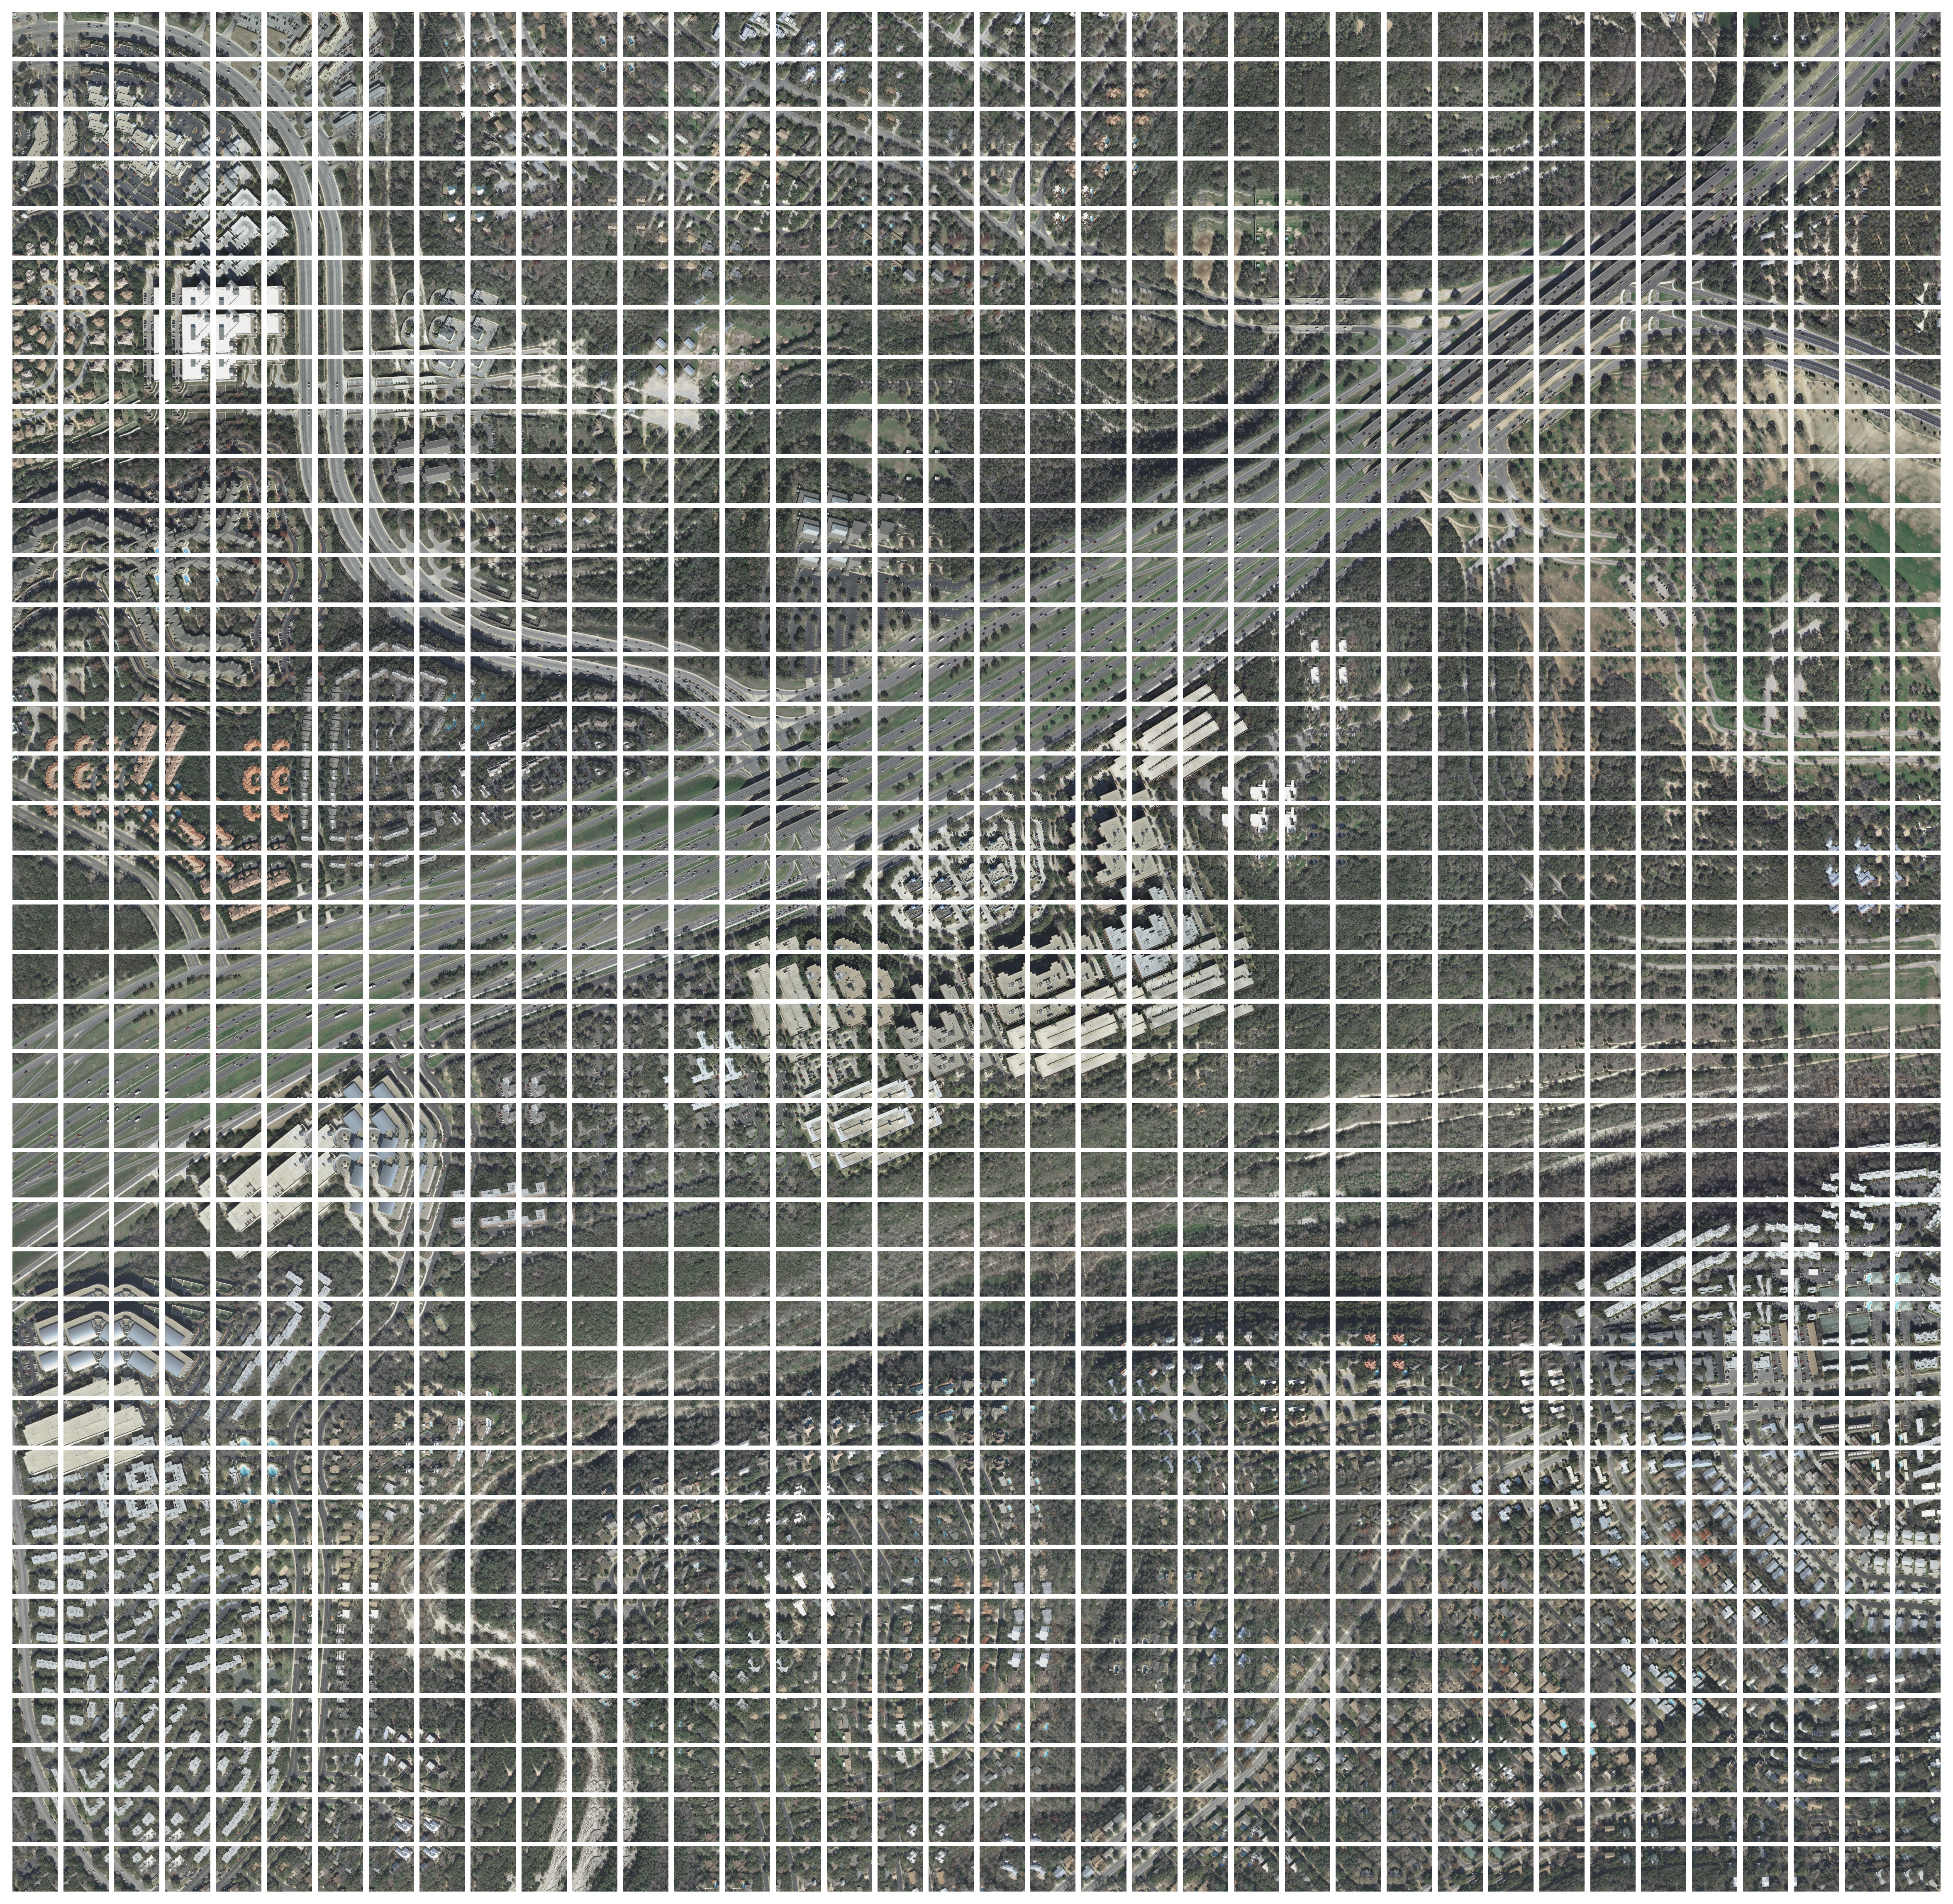
\includegraphics[width=1.0\linewidth]{Podprobki.png}
    \captionsetup{format=hang}
    \caption{Wybrane zdjęcie pochodzące ze zbioru walidacyjnego rozbite na 1444 podpóbki}
    \label{fig:podprob1}
\end{figure}

\cell
Mając do dyspozycji wszystkie 1444 podpróbki zdjęcia bazowego można było przystąpić do generowania predykcji masek dla każdej z tych podpróbek.
\vspace{1.5cm}

\cell
\begin{lstlisting}[name=Rozdzial3.1, language=Python]
def get_all_preds(reshp_img):
  fin_trans = transforms.Compose([transforms.ToTensor(), 
                                  transforms.Normalize(mean_rgbs, std_rgbs)])
  fin_preds = np.zeros((reshp_img.shape[0], sample_res, sample_res))

  for i in range(0, reshp_img.shape[0], batch_s):
    if i + batch_s > reshp_img.shape[0]:
      continue
    input = reshp_img[i:(i + batch_s), ...]
    trans_input = torch.zeros((input.shape[0], input.shape[3], input.shape[1], 
                              input.shape[2]))
    for j in range(input.shape[0]):
      trans_input[j, ...] = fin_trans(input[j, ...])
    with torch.no_grad():
      pred_base = trnd_model(trans_input.to(device))

    pred_sigm = torch.sigmoid(pred_base).data.cpu().numpy()
    fin_preds[i:(i + batch_s), ...] = pred_sigm
    
  return fin_preds
\end{lstlisting}


\cell
Aby móc efektywnie połączyć uzyskane predykcje w jedną łączną maskę o rozdzielczości $\textit{5000x5000}$ postanowiono skorzystać z dwuwymiarowych okien Hanna zdefiniowanych szerzej w artykule Nicolasa Pielawskiego oraz Caroliny Wählby \textit{Introducing Hann windows for reducing edge-effects in patch-based image segmentation} \cite{pielawski}.

\cell
\begin{lstlisting}[name=Rozdzial3.1, language=Python]
hann_wnd_b = np.zeros((sample_res, sample_res), dtype=float)
hann_wnd_up = np.zeros((sample_res, sample_res), dtype=float)
hann_wnd_down = np.zeros((sample_res, sample_res), dtype=float)
hann_wnd_left = np.zeros((sample_res, sample_res), dtype=float)
hann_wnd_right = np.zeros((sample_res, sample_res), dtype=float)
hann_wnd_up_l = np.zeros((sample_res, sample_res), dtype=float)
hann_wnd_down_l = np.zeros((sample_res, sample_res), dtype=float)
hann_wnd_up_r = np.zeros((sample_res, sample_res), dtype=float)
hann_wnd_down_r = np.zeros((sample_res, sample_res), dtype=float)
\end{lstlisting}


\cell
Autorzy tego artykułu zaproponowali algorytm łączenia podpróbek zdjęć w jedno łączne zdjęcie w czasie realizowania zadań z zakresu semantycznej segmentacji. Ich pomysł opierał się na przemnażaniu predykcji uzyskanych dla poszczególnych podpróbek przez dwuwymiarowe okna Hanna, stanowiące $\textit{de facto}$ macierz wag, która główny nacisk kładzie na predykcje znajdujące się w środku podpróbki - w ten sposób redukowany jest efekt złych predykcji krawędzi.

\cell
\begin{lstlisting}[name=Rozdzial3.1, language=Python]
def hann_up_down_left_right(i, j, h_part, v_part):
  if j < sample_res / 2:
    hann_wnd_up[j, i] = 0.5 * h_part
  else:
    hann_wnd_up[j, i] = 0.25 * h_part * v_part
  
  if j > sample_res / 2:
    hann_wnd_down[j, i] = 0.5 * h_part
  else:
    hann_wnd_down[j, i] = 0.25 * h_part * v_part

  if i < sample_res / 2:
    hann_wnd_left[j, i] = 0.5 * v_part
  else:
    hann_wnd_left[j, i] = 0.25 * h_part * v_part
  
  if i > sample_res / 2:
    hann_wnd_right[j, i] = 0.5 * v_part
  else:
    hann_wnd_right[j, i] = 0.25 * h_part * v_part
\end{lstlisting}


\cell
Nicolas Pielawski i Caroline Wählby zaproponowali również modyfikacje bazowego dwuwymiarowego okna Hanna, dla przypadków gdy predykcja pochodzi z podpróbki znajdującej się na krawędzi zdjęcia bazowego, tak żeby w takich przypadkach położyć nacisk na predykcje znajdujące się na krawędziach podpróbki.

\cell
\begin{lstlisting}[name=Rozdzial3.1, language=Python]
def hann_up_l_up_r(i, j, h_part, v_part):
  if i <= sample_res / 2 and j <= sample_res / 2:
    hann_wnd_up_l[j, i] = 1
  elif i > sample_res / 2 and j < sample_res / 2:
    hann_wnd_up_l[j, i] = 0.5 * h_part
  elif i < sample_res / 2 and j > sample_res / 2:
    hann_wnd_up_l[j, i] = 0.5 * v_part
  else:
    hann_wnd_up_l[j, i] = 0.25 * h_part * v_part

  if i >= sample_res / 2 and j <= sample_res / 2:
    hann_wnd_up_r[j, i] = 1
  elif i < sample_res / 2 and j < sample_res / 2:
    hann_wnd_up_r[j, i] = 0.5 * h_part
  elif i > sample_res / 2 and j > sample_res / 2:
    hann_wnd_up_r[j, i] = 0.5 * v_part
  else:
    hann_wnd_up_r[j, i] = 0.25 * h_part * v_part
\end{lstlisting}


\cell
W ten sposób uzyskano 9 wariantów dwuwymiarowego okna Hanna, których zastosowanie zależało od tego gdzie dana podpróbka znajduje się na obrazie bazowym. Funkcje $\textit{hann$\_$up$\_$down$\_$eft$\_$right}$, $\textit{hann$\_$up$\_$l$\_$up$\_$r}$ oraz $\textit{hann$\_$down$\_$r$\_$down$\_$l}$ zawierają implementacje poszczególnych dwuwymiarowych okien Hanna.

\cell
\begin{lstlisting}[name=Rozdzial3.1, language=Python]
def hann_down_r_down_l(i, j, h_part, v_part):
  if i >= sample_res / 2 and j >= sample_res / 2:
    hann_wnd_down_r[j, i] = 1
  elif i < sample_res / 2 and j > sample_res / 2:
    hann_wnd_down_r[j, i] = 0.5 * h_part
  elif i > sample_res / 2 and j < sample_res / 2:
    hann_wnd_down_r[j, i] = 0.5 * v_part
  else:
    hann_wnd_down_r[j, i] = 0.25 * h_part * v_part
  if i <= sample_res / 2 and j >= sample_res / 2:
    hann_wnd_down_l[j, i] = 1
  elif i > sample_res / 2 and j > sample_res / 2:
    hann_wnd_down_l[j, i] = 0.5 * h_part
  elif i < sample_res / 2 and j < sample_res / 2:
    hann_wnd_down_l[j, i] = 0.5 * v_part
  else:
    hann_wnd_down_l[j, i] = 0.25 * h_part * v_part
\end{lstlisting}


\cell
Rysunek \ref{fig:hann1} prezentuje wizualizację wszystkich dziewięciu okien Hanna, które w dalszej części niniejszego podrozdziału posłużą do połączenia predykcji uzyskanych z podpróbek w jedną łączną maskę predykcji.
\vspace{1cm}

\cell
\begin{lstlisting}[name=Rozdzial3.1, language=Python]
for i in range(sample_res):
  for j in range(sample_res):
    h_part = (1 - np.cos((2 * np.pi * i) / (sample_res - 1)))
    v_part = (1 - np.cos((2 * np.pi * j) / (sample_res - 1)))
    hann_wnd_b[j, i] = 0.25 * h_part * v_part
    hann_up_down_left_right(i, j, h_part, v_part)
    hann_up_l_up_r(i, j, h_part, v_part)
    hann_down_r_down_l(i, j, h_part, v_part)
\end{lstlisting}

\begin{figure}[!h]
    \centering \includegraphics[width=1.0\linewidth]{Okna Hanna.png}
    \captionsetup{format=hang}
    \caption{Wizualizacja dziewięciu okien Hanna 2D służących do właściwego ważenia predykcji poszczególnych fragmentów zdjęcia bazowego}
    \label{fig:hann1}
\end{figure}
\vspace{1cm}

\cell
\begin{lstlisting}[name=Rozdzial3.1, language=Python]
f2, axarr2 = plt.subplots(nrows=3, ncols=3, figsize=(25, 25))
axarr2[0, 0].imshow(hann_wnd_up_l, cmap='viridis')
axarr2[1, 0].imshow(hann_wnd_left, cmap='viridis')
axarr2[2, 0].imshow(hann_wnd_down_l, cmap='viridis')
axarr2[0, 1].imshow(hann_wnd_up, cmap='viridis')
axarr2[1, 1].imshow(hann_wnd_b, cmap='viridis')
axarr2[2, 1].imshow(hann_wnd_down, cmap='viridis')
axarr2[0, 2].imshow(hann_wnd_up_r, cmap='viridis')
axarr2[1, 2].imshow(hann_wnd_right, cmap='viridis')
axarr2[2, 2].imshow(hann_wnd_down_r, cmap='viridis')
axarr2[0, 0].axis('off')
axarr2[1, 0].axis('off')
axarr2[2, 0].axis('off')
axarr2[0, 1].axis('off')
axarr2[1, 1].axis('off')
axarr2[2, 1].axis('off')
axarr2[0, 2].axis('off')
axarr2[1, 2].axis('off')
axarr2[2, 2].axis('off')
plt.savefig('Okna Hanna.png', dpi=300, bbox_inches='tight')
\end{lstlisting}

\cell
Funkcja $\textit{choose$\_$proper$\_$hann}$ służy do wyboru odpowiedniego dwuwymiarowego okna Hanna, w zależności od tego, z której części bazowego zdjęcia walidacyjnego dana podpróbka została pobrana.

\cell
\begin{lstlisting}[name=Rozdzial3.1, language=Python]
def choose_proper_hann(i, j, max_shp):
  if j == 0 and i == 0:
    curr_hann = hann_wnd_up_l
  elif i == 0 and j != 0 and j != max_shp - 1:
    curr_hann = hann_wnd_up
  elif i == 0 and j == max_shp - 1:
    curr_hann = hann_wnd_up_r
  elif j == 0 and i != 0 and i != max_shp - 1:
    curr_hann = hann_wnd_left
  elif j == 0 and i == max_shp - 1:
    curr_hann = hann_wnd_down_l
  elif j == max_shp - 1 and i != 0 and i != max_shp - 1:
    curr_hann = hann_wnd_right
  elif j == max_shp - 1 and i == max_shp - 1:
    curr_hann = hann_wnd_down_r
  elif j != 0 and j != max_shp - 1  and i == max_shp - 1:
    curr_hann = hann_wnd_down
  else:
    curr_hann = hann_wnd_b
  return curr_hann
\end{lstlisting}


\cell
Przy pomocy funkcji $\textit{get$\_$fin$\_$mask}$ realizowane jest generowanie finalnej maski dla poszczególnych zdjęć ze zbioru walidacyjnego. Funkcja ta przechodzi przez predykcje wygenerowane dla wszystkich podpróbek, przemnaża je przez odpowiednie okna Hanna i~nanosi we właściwym miejscu finalnej maski $\textit{5000x5000}$. 

\cell
\begin{lstlisting}[name=Rozdzial3.1, language=Python]
def get_fin_mask(fin_preds, Gy, Gx, wnd_h, wnd_w, img_h, img_w, Sy, Sx):
  rshp_fin_preds = fin_preds.reshape((Gy, Gx, wnd_h, wnd_w))
  fin_image_mask = np.zeros((img_h, img_w))
  end_x = sample_res
  strt_x = 0
  for i in range(Gy):
    end_y = sample_res
    strt_y = 0
    for j in range(Gx):
      curr_p = rshp_fin_preds[i, j]
      curr_h = choose_proper_hann(i, j, Gy)
      fin_image_mask[strt_x:end_x, strt_y:end_y] += np.multiply(curr_p, curr_h)
      strt_y += Sy
      end_y += Sy
    strt_x += Sx
    end_x += Sx
  return fin_image_mask
\end{lstlisting}

\subsection{Pomiar efektywności sieci \emph{GML-Net}}

\cell
Poniższe obrazy wizualizują skuteczność sieci $\textit{GML-Net}$ w detekcji budynków na zdjęciach lotniczych na przykładzie losowo wybranego zdjęcia ze zbioru walidacyjnego.

\cell
\begin{lstlisting}[name=Rozdzial3.1, language=Python]
imgs_arr = pd.read_csv("m_inf_v.csv", header=None).values
img_n = 1
final_f1s = []
final_iou = []
final_acc = []
final_ssim = []
pred_time = []
img_time = []
img, msk, wnd_h, wnd_w, nm_cls, img_h, img_w, Sy, Sx = g_prms(imgs_arr, img_n)
wnd_img, Gx, Gy = get_wnds(img, msk, wnd_h, wnd_w, nm_cls, img_h, img_w, Sy, Sx)
fin_preds = get_all_preds(wnd_img)
f_img_msk = get_fin_mask(fin_preds, Gy, Gx, wnd_h, wnd_w, img_h, img_w, Sy, Sx)
\end{lstlisting}

\begin{figure}[!h]
    \centering 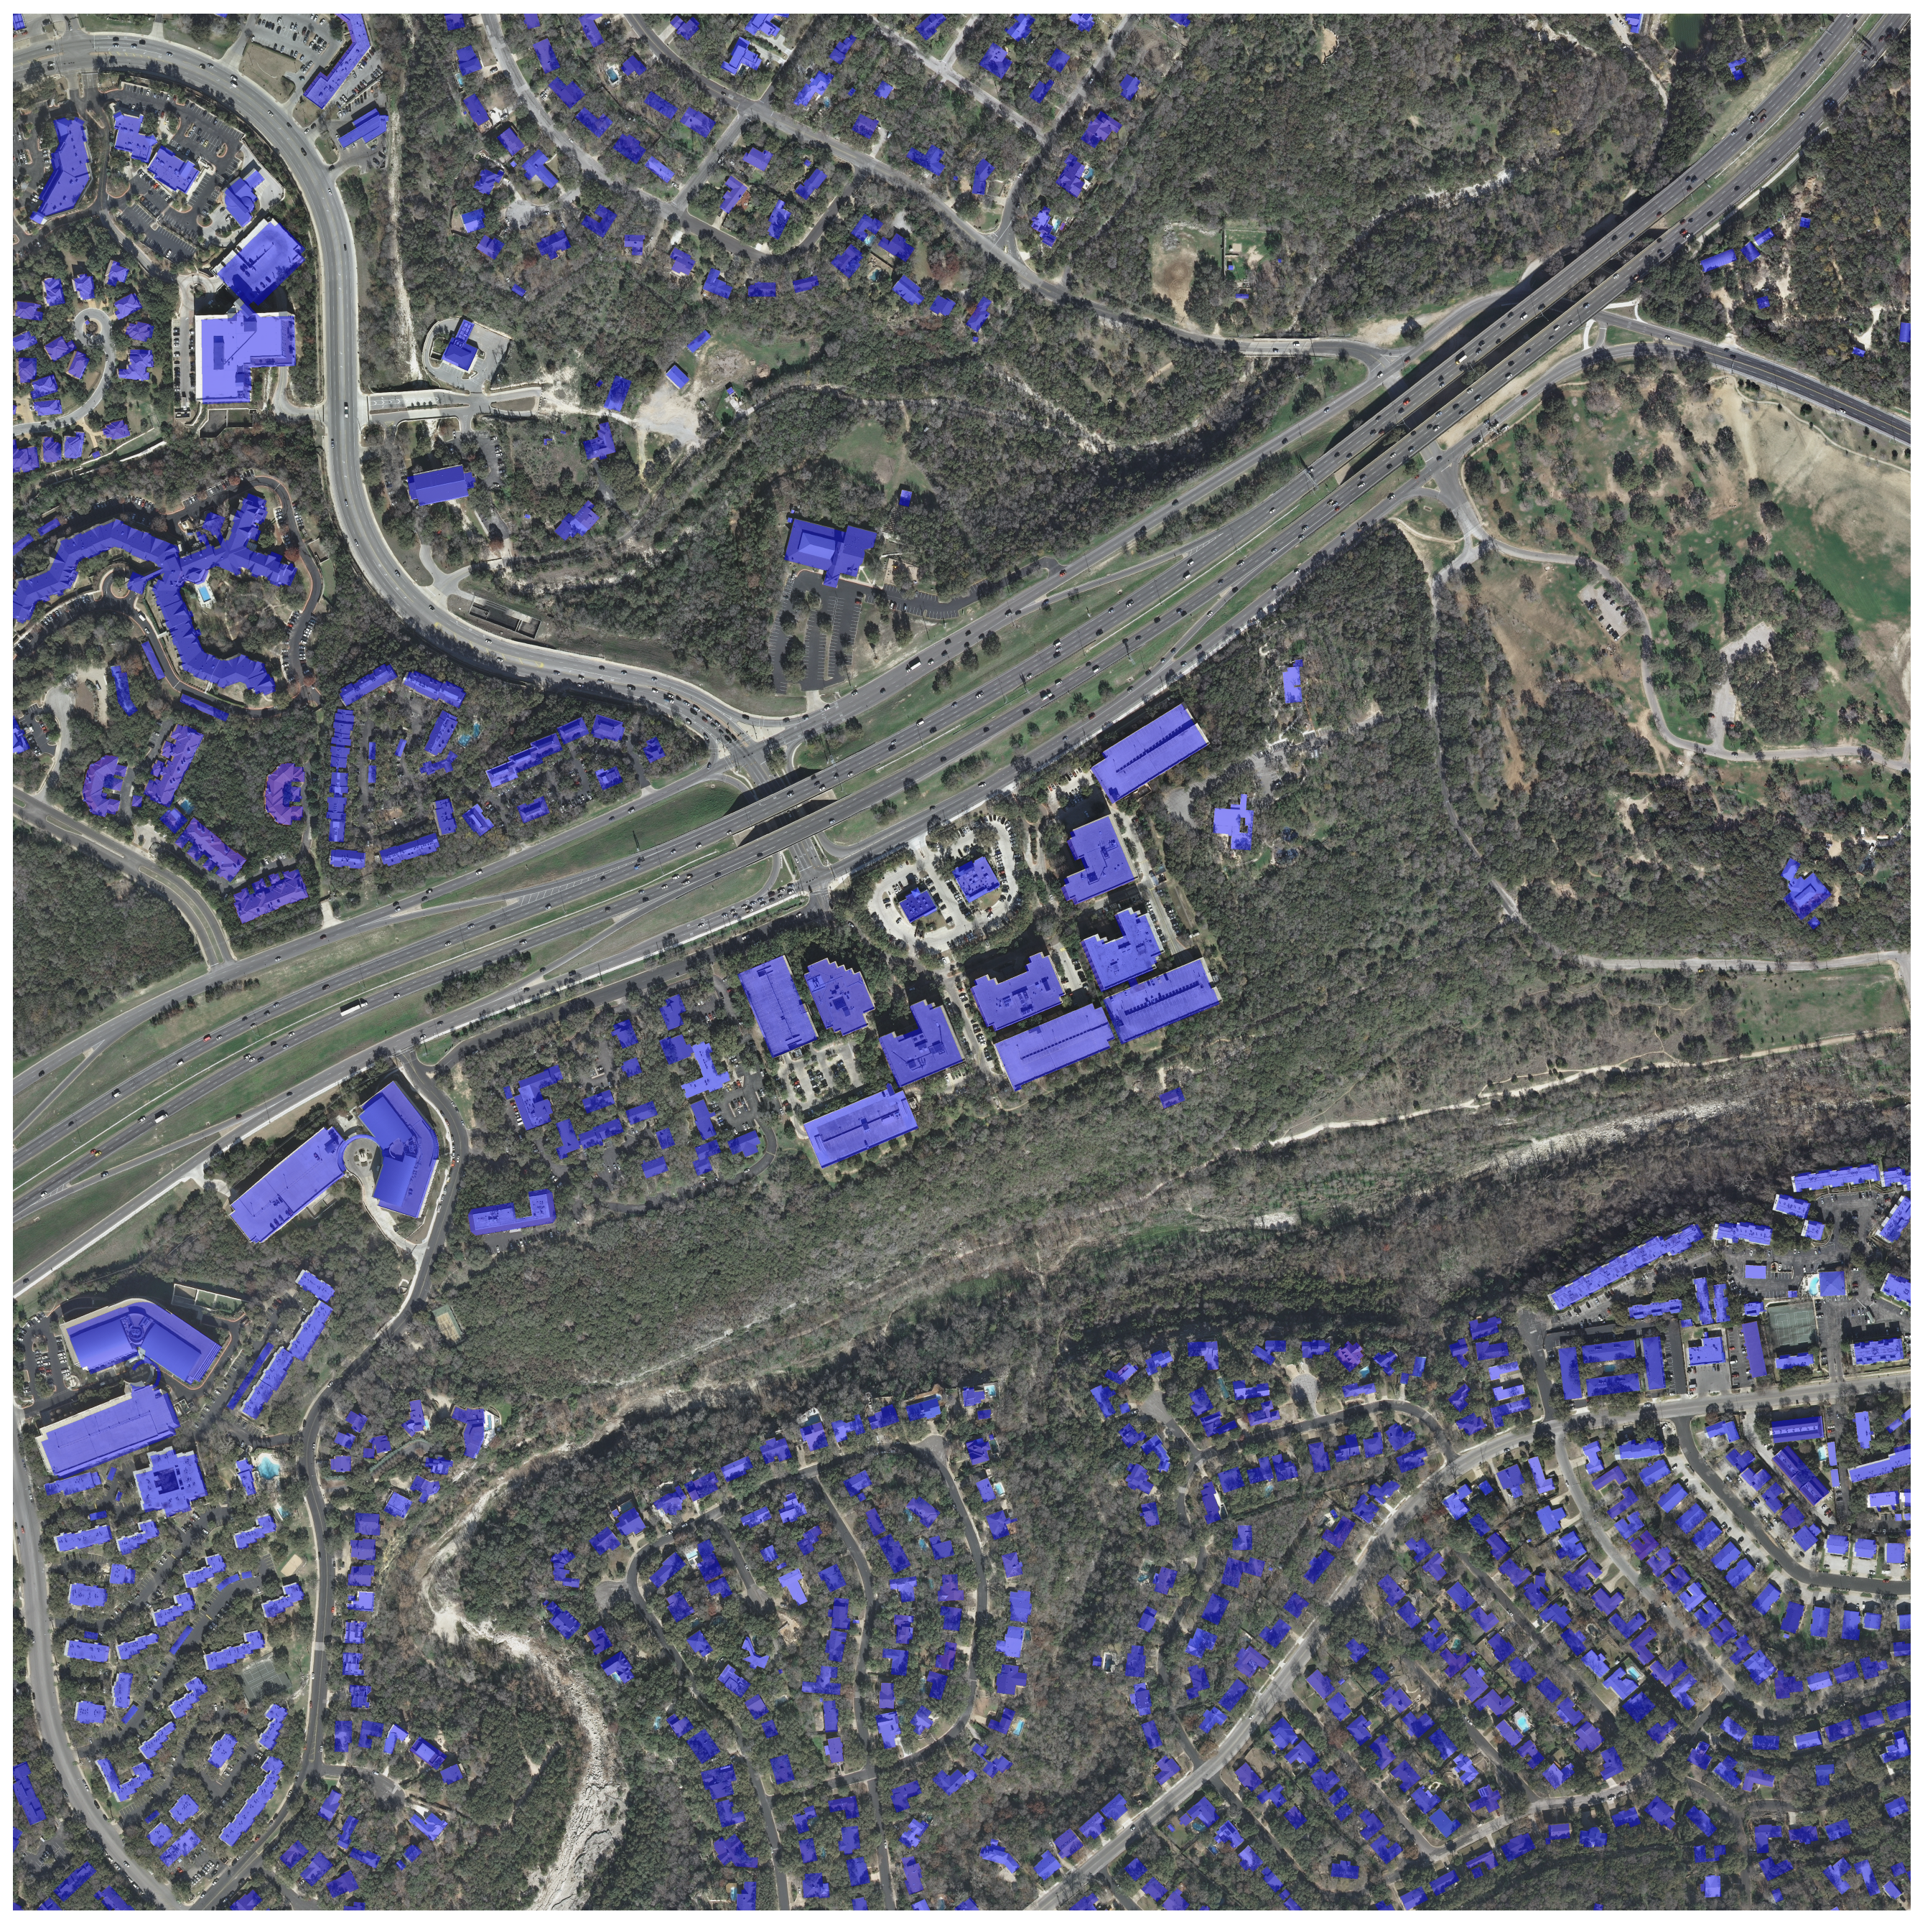
\includegraphics[width=1.0\linewidth]{Maska GT.png}
    \captionsetup{format=hang}
    \caption{Oryginalna maska (\textit{ground truth})}
    \label{fig:predGT1}
\end{figure}

\cell
Porównanie wizualne rysunku \ref{fig:predGT1} z rysunkiem \ref{fig:predGT2} wskazuje, iż różnice w predykcji maski przez sieć $\textit{GML-Net}$ a faktyczną maską $\textit{ground truth}$ nie są istotne.

\begin{figure}[!h]
    \centering 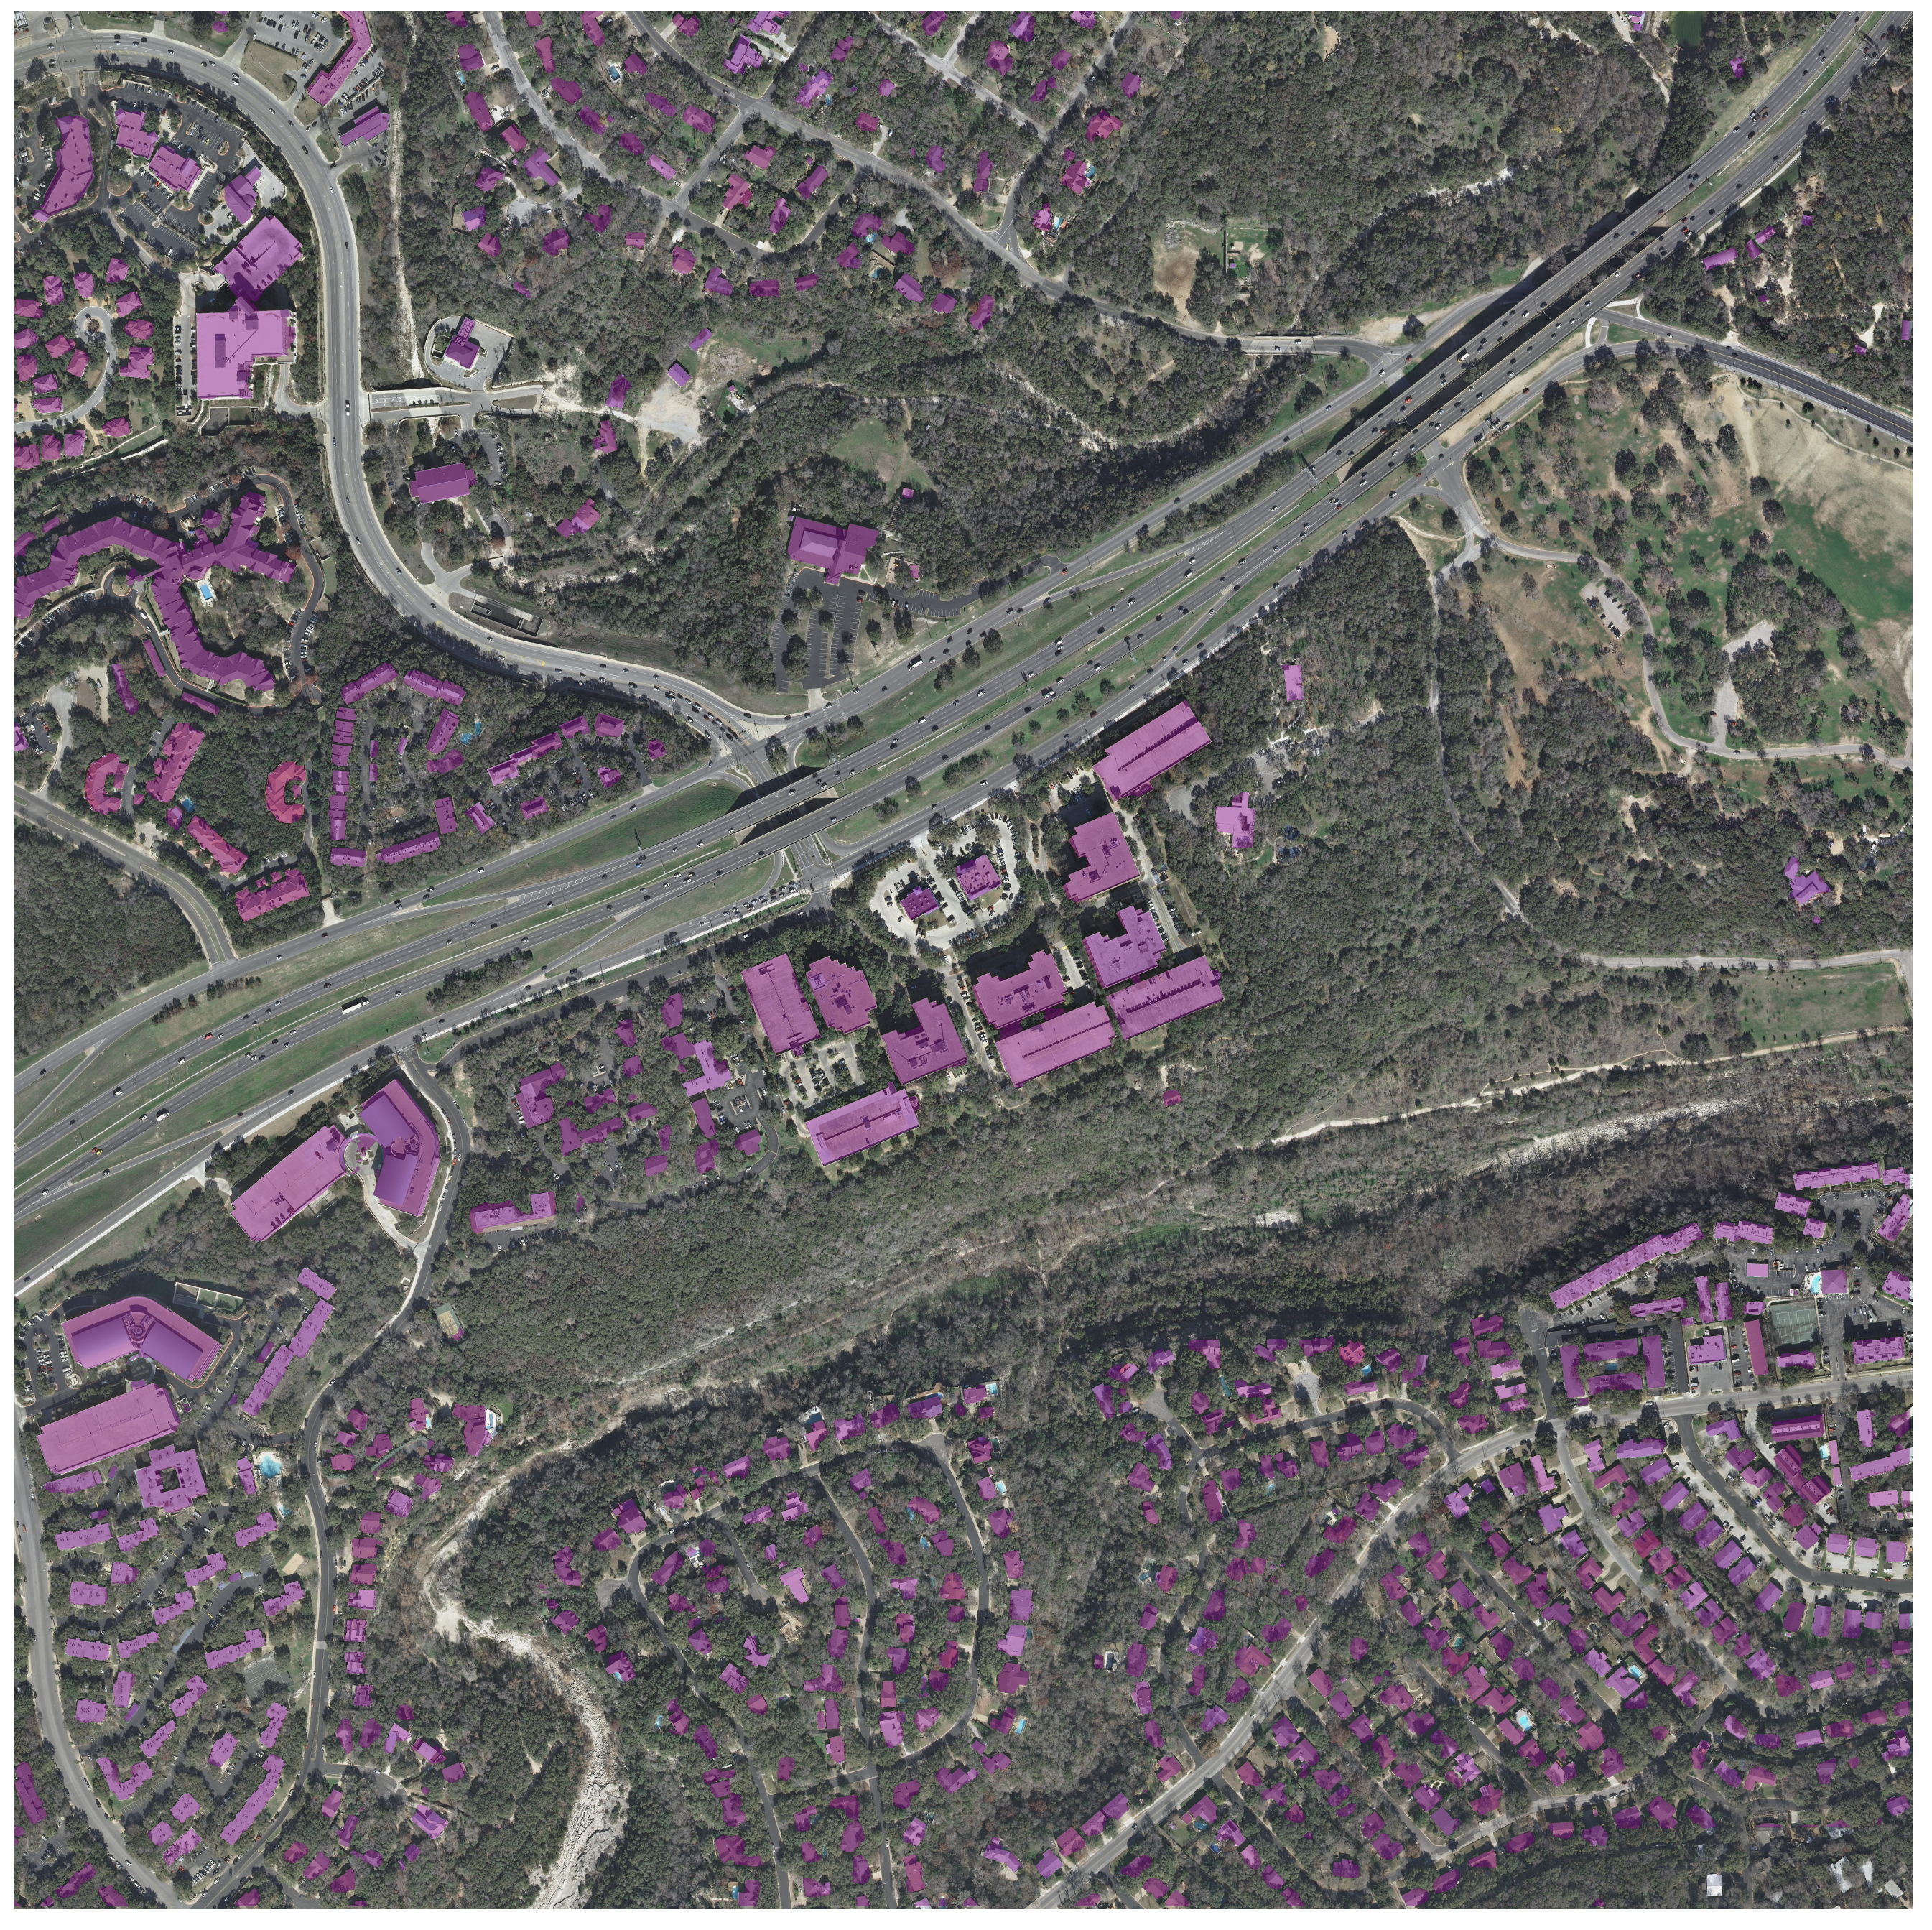
\includegraphics[width=1.0\linewidth]{Predykcja sieci.png}
    \captionsetup{format=hang}
    \caption{Maska wygenerowana przez sieć \textit{GML-Net}}
    \label{fig:predGT2}
\end{figure}

\cell
\begin{lstlisting}[name=Rozdzial3.1, language=Python]
img_rgba = np.ones((img.shape[0], img.shape[1], 4), dtype=np.uint8) * 255
img_rgba[..., :3] = img
mask_rgba = np.zeros((img.shape[0], img.shape[1], 4), dtype=np.uint8)
mask_rgba[msk == 255, ...] = [0, 0, 255, 180]
pred_mask_rgba = np.zeros((img.shape[0], img.shape[1], 4), dtype=np.uint8)
pred_mask_rgba[f_img_msk > loss_thres, ...] = [128, 0, 128, 180]

f2, axarr2 = plt.subplots(nrows=1, ncols=2, figsize=(25, 25))
axarr2[0].set_title("Maska ground truth\n", color='black', fontweight="bold",
                    fontsize=25)
axarr2[0].imshow(img_rgba)
axarr2[0].imshow(mask_rgba, alpha=0.6)
axarr2[0].axis('off')
axarr2[1].imshow(img_rgba)
axarr2[1].imshow(pred_mask_rgba, alpha=0.6)
axarr2[1].axis('off')
axarr2[1].set_title("Maska uzyskana z sieci GML-Net\n", color='black', 
                    fontweight="bold", fontsize=25)
                    
plt.savefig('Predykacja vs. maska.png', dpi=300, bbox_inches='tight')
\end{lstlisting}

\cell
\begin{lstlisting}[name=Rozdzial3.1, language=Python]
def calc_metrics(f_img_msk, msk):
  prd2 = f_img_msk > loss_thres
  trgt2 = msk == 255
  intrs = (prd2 * trgt2).sum()
  
  f1s = torch.True_divide(2. * intrs, prd2.sum() + trgt2.sum())
  f1s = f1s.cpu().numpy().item(0)
  union = (prd2 + trgt2).sum()
  
  iou = torch.True_divide(intrs, union).cpu().numpy().item(0)
  acc = torch.True_divide(intrs + (~prd2 * ~trgt2).sum(), prd2.size)
  acc = acc.cpu().numpy().item(0)
  
  prd3 = torch.tensor(np.expand_dims(prd2, axis=0)).cuda()
  trgt3 = torch.tensor(np.expand_dims(trgt2, axis=0)).cuda()
  ssim = ssim_index(prd3, trgt3).cpu().numpy().item(0)
  
  return f1s, iou, acc, ssim

f1s, iou, acc, ssim = calc_metrics(f_img_msk, msk)
\end{lstlisting}


\cell
Wartości poszczególnych metryk wyliczone dla powyższego losowego zdjęcia pochodzącego ze zbioru walidacyjnego potwierdzają obserwacje wizualne wskazujące na dobrą jakość predykcji. Wartości tych metryk są następujące: $\textit{OA}$ = 97,66$\%$, $\textit{IoU}$ = 80,10$\%$, $\textit{F1S}$ = 88,95$\%$ oraz $\textit{SSIM}$ = 96,26$\%$.
\vspace{1cm}

\cell
\begin{lstlisting}[name=Rozdzial3.1, language=Python]
for i in range(len(imgs_arr)):
  since0 = time.time()
  img, msk, wnd_h, wnd_w, nm_cls, img_h, img_w, Sy, Sx = g_prms(imgs_arr, i)
  wnd_i, Gx, Gy = get_wnds(img, msk, wnd_h, wnd_w, nm_cls, img_h, img_w, 
                           Sy, Sx)
  fin_p = get_all_preds(wnd_i)
  since1 = time.time()
  f_img_msk = get_fin_mask(fin_p, Gy, Gx, wnd_h, wnd_w, img_h, img_w,
                           Sy, Sx)
  pred_time += [time.time() - since1]
  img_time += [time.time() - since0]
  f1s, iou, acc, ssim = calc_metrics(f_img_msk, msk)                                                        
  final_f1s += [f1s]
  final_iou += [iou]
  final_acc += [acc]
  final_ssim += [ssim]

joined_time = sum(img_time)
av_img_time = sum(img_time) / len(imgs_arr)
avg_pred_time = sum(pred_time) / (len(imgs_arr) * Gx * Gy)
\end{lstlisting}

\cell
Sieć $\textit{GML-Net}$ osiągnęła zadowalającą finalną skuteczność na zbiorze walidacyjnym przy predykcji masek o rozmiarach $\textit{5000x5000}$ - uzyskano następujące finalne wartości metryk: \textit{OA} = 96,44\%, \textit{IoU} = 75,97\%, \textit{F1S} = 86,07\% oraz \textit{SSIM} = 94,55\%. Wyniki te zostały uzyskane przy średnim czasie generowania predykcji jednej maski \emph{256x256} na poziomie 0,0003 sekundy oraz średnim czasie generowania predykcji maski łącznego obrazka \emph{5000x5000} na poziomie 15 sekund.
\vspace{0.5cm}

\begin{table}[!h]
\centering
\begin{tabular}{|M{3cm}|M{5.5cm}|M{5.5cm}|}
\hline
\rowcolor{gray!50}
\textbf{Rodzaj metryki} & \textbf{Wyniki dla masek 256x256} & \textbf{Wyniki dla masek 5000x5000} \\ 
 \hline 
\textbf{OA} & 97,08\% & 96,44\% \\
 \hline 
\textbf{IoU} & 82,42\% & 75,97\% \\
 \hline 
\textbf{F1S} & 88,22\% & 86,07\% \\
 \hline 
\textbf{SSIM} & 95,46\% & 94,55\% \\
 \hline 
\end{tabular}
\caption{Podsumowanie różnic pomiędzy metrykami jakości predykcji sieci \textit{GML-Net} dla masek \emph{256x256} a~tymi samymi metrykami dla masek \emph{5000x5000}.}
\label{tab:tabela2}
\end{table}

Jak można się było spodziewać metryki jakości predykcji modelu wyliczane na poziomie pełnych zdjęć o wysokiej rozdzielczości są gorsze od metryk wyliczanych na poziomie podpróbek o rozdzielczości $\textit{256x256}$. Ogólna dokładność pogarsza się o 0,64 punktu procentowego, współczynnik podobieństwa Jaccarda spada aż o 6,45 p.p., wynik $\textit{F1}$ jest niższy o 2,35 p.p. a indeks podobieństwa strukturalnego jest gorszy o 0,91 p.p. 

\subsection{Uzyskane wyniki na tle literatury badawczej}

Tabela \ref{tab:tabela3} przywołuje ponownie wyniki uzyskane na zbiorze \textit{Inria Aerial Image Labeling Dataset} przez autorów, których prace zostały omówione w~przeglądzie literatury. Uzyskane przez nich wyniki dotyczą zbioru testowego \emph{IAILD}, natomiast opisywane, jak dotąd, wartości metryk jakości predykcji sieci \textit{GML-Net} dotyczyły wyłącznie zbioru walidacyjnego. Aby więc móc porównywać skuteczność modelu opisywanego w~bieżącej pracy na tle skuteczności innych modeli, należałoby policzyć odpowiednie metryki jakości predykcji sieci \textit{GML-Net} na zbiorze testowym.

\vspace{0.5cm}
\begin{table}[!h]
\centering
\begin{tabular}{|M{7cm}|M{4cm}|}
\hline
\rowcolor{gray!50}
\textbf{Tytuł artykułu} & \textbf{Uzyskane wyniki} \\ \hline &\\[0.1cm]

\emph{Multi-Task Learning for Segmentation of Building Footprints with Deep Neural Networks} \cite{bischke} & \makecell{OA: 95.17\% \\ IoU: 70.14\%} \\[0.1cm] &\\ \hline &\\[0.1cm]

\emph{Semantic Segmentation from Remote Sensor Data and the Exploitation of Latent Learning for Classification of Auxiliary Tasks} \cite{chatterjee} & \makecell{OA: 97.14\% \\ IoU: 80.32\%} \\[0.1cm] &\\ \hline &\\[0.1cm]

\emph{Building Footprint Generation by Integrating Convolution Neural Network with Feature Pairwise Conditional Random Field (FPCRF)} \cite{zhu} & \makecell{OA: 95.81\% \\ F1S: 87.65\% \\ IoU: 74.79\%} \\[0.1cm] &\\ \hline &\\[0.1cm]

\emph{Polygonal Building Segmentation by Frame Field Learning} \cite{girard} & \makecell{IoU: 78.00\%} \\[0.1cm] &\\ \hline
\end{tabular}
\caption{Podsumowanie wyników uzyskanych na zbiorze \textit{Inria Aerial Image Labeling Dataset} przez autorów innych badań zajmujących się problematyką detekcji budynków na zdjęciach lotniczych.}
\label{tab:tabela3}
\end{table}

Niestety nie można zrobić tego samodzielnie, gdyż autorzy zbioru \textit{Inria Aerial Image Labeling Dataset} nie udostępnili masek 
\emph{ground truth} dla zbioru testowego. Przygotowali oni jednak formularz na stronie internetowej \emph{IAILD} (\url{https://www.lri.fr/~gcharpia/aerial_benchmark}), w~ramach którego możliwe jest przesłanie, do autorów wykorzystywanego w~bieżącej pracy zbioru danych, predykcji 180~masek dla zbioru testowego. Po wysłaniu takich danych, po pewnym czasie, autorzy \textit{Inria Aerial Image Labeling Dataset} odsyłają, na podany w~formularzu adres \emph{e-mail}, wyliczone przez nich wartości metryk \emph{IoU} oraz \emph{OA}, w~podziale na wyniki dla poszczególnych miast ze zbioru testowego. 

\begin{table}[!h]
\centering
\begin{tabular}{|M{7cm}|M{3cm}|M{3cm}|}
\hline
\rowcolor{gray!50}
\textbf{Miasto} & \textbf{OA} & \textbf{IoU} \\ \hline
Bellingham & 97,11\% & 71,39\% \\ \hline
Bloomington & 97,34\% & 71,83\% \\ \hline
Innsbruck & 96,99\% & 74,89\% \\ \hline
San Francisco & 91,72\% & 74,98\% \\ \hline
Tyrol Wschodni & 98,01\% &  77,85\% \\ \hline
\textbf{Łącznie:} & \textbf{96,23\%} & \textbf{74,42\%} \\ \hline
\end{tabular}
\caption{Podsumowanie wyników sieci \textit{GML-Net} dla zbioru testowego \textit{IAILD}}
\label{tab:tabela4}
\end{table}

Tabela \ref{tab:tabela4} przedstawia wskaźniki jakości predykcji sieci \textit{GML-Net} dla zbioru testowego \textit{IAILD}, wyliczone przez autorów tego zbioru po przesłaniu im 180~predykcji masek. Jak widać omawiana w~bieżącym rozdziale sieć osiągnęła łączną skuteczność mierzoną przy pomocy metryki \textit{OA} na poziomie 96,23\% a~mierzoną przy pomocy metryki \textit{IoU} na poziomie 74,42\%. Najlepsze wyniki sieć \textit{GML-Net} uzyskała dla miasta Tyrol Wschodni, a najgorsze dla miast San Francisco (pod kątem \textit{OA}) oraz Bellingham (pod kątem \textit{IoU}). 

Porównując uzyskane wyniki do wyników zaprezentowanych w~przeglądzie literatury można śmiało stwierdzić, iż sieć \textit{GML-Net} jest w~stanie generować wyniki o~zbliżonej jakości do modeli przedstawionych w~literaturze, odstając o~zaledwie niecały punkt procentowy od najlepszego wyniku pod kątem metryki \textit{OA} i~o~niecałe sześć punktów procentowych pod kątem metryki \textit{IoU}. Wyniki uzyskane przez sieć \textit{GML-Net} można również porównać do wyników prezentowanych przez autorów zbioru  \textit{Inria Aerial Image Labeling Dataset} na ich stronie internetowej (\url{https://project.inria.fr/aerialimagelabeling/leaderboard}). Znajduje się tam tabela przedstawiająca wartości uzyskiwanych metryk \textit{OA} i \textit{IoU} dla 110~modeli, których autorzy zgodzili się na publikację wskaźników jakości predykcji ich sieci. Średnia wartość ogólnej dokładności dla tych 110~modeli wynosi 95,46\%, a~średnia wartość indeksu Jaccarda wynosi 70,02\%, co oznacza, iż sieć \textit{GML-Net} uzyskuje wyniki istotnie wyższe od średnich dla tego zbioru - mówiąc dokładniej, zajmuje 29. miejsce pod kątem \textit{OA} oraz 30 pod kątem \textit{IoU}.

\clearpage
\section{Zakończenie}

Niniejsza praca podejmowała problematykę detekcji budynków na zdjęciach lotniczych przy użyciu głębokich sieci neuronowych. Praca ta w~pierwszych rozdziałach skupiała się na zdefiniowaniu najważniejszych pojęć związanych z~głębokim uczeniem, przedstawieniem jego podstaw teoretycznych, historii oraz najistotniejszych architektur z~nim związanych. Kolejne rozdziały zostały poświęcone przeglądowi literatury badawczej z~zakresu badanej problematyki oraz definicji własnej głębokiej sieci neuronowej o~nazwie \textit{GML-Net}. Całość została zwieńczona rozdziałem opisującym sposób generacji finalnych predykcji oraz porównującym uzyskane wyniki do wyników przedstawionych literaturze badawczej.

Zaprezentowana w~bieżącej pracy sieć \textit{GML-Net} pozwoliła na uzyskanie zadowalającej skuteczności w~detekcji budynków na zdjęciach lotniczych pochodzących ze zbioru \textit{Inria Aerial Image Labeling Dataset}. Nie udało się w~prawdzie osiągnąć lepszych rezultatów niż aktualne wyniki \textit{state of art} zaprezentowane w~pracy \textit{Semantic Segmentation from Remote Sensor Data and the Exploitation of Latent Learning for Classification of Auxiliary Tasks} \cite{chatterjee}, ale mimo to wyniki uzyskane przy pomocy sieci \textit{GML-Net} można uznać za satysfakcjonujące. Za duże pole do dalszego rozwoju uzyskanej sieci można uznać sposób łączenia predykcji masek o~rozdzielczości \emph{256x256} w~jedną łączną maskę o~rozdzielczości \emph{5000x5000}, gdyż w~tym procesie skuteczność predykcji istotnie się pogarszała, szczególnie patrząc przez pryzmat metryki \textit{Intersection over Union}. 

Za duże zalety sieci \textit{GML-Net} można natomiast uznać jej ciekawą architekturę wykorzystująca elementy sieci \textit{ResNet}, \textit{U-Net} oraz \textit{ICT-Net}, a także nowatorską funkcję straty stanowiąca ważoną sumę \textit{Binary Cross-Entropy Loss}, \textit{Dice Loss} oraz \textit{Lovász hinge loss}. Stąd też, za uprawnione wydaje się stwierdzenie, iż zaprezentowana w~niniejszej pracy głęboka sieć neuronowa \textit{GML-Net} wnosi nowe, ciekawe spojrzenie do literatury podejmującej problematykę detekcji budynków na zdjęciach lotniczych.
                           
%---------------------------------------------------------------
% Literatura
%---------------------------------------------------------------
\clearpage
\newrefcontext[sorting=nty]
\printbibliography

%---------------------------------------------------------------
% Spisy
%---------------------------------------------------------------
\newpage
\pagestyle{plain}
\vspace{0.8cm}
\acronymlist
\acronym{ADALINE}{ang. \emph{Adaptive Linear Neuron}}
\acronym{AI}{ang. \emph{Artificial Intelligence}}
\acronym{BCE}{ang. \emph{Binary Cross-Entropy}}
\acronym{BGD}{ang. \emph{Batch Gradient Descent}}
\acronym{BSGD}{ang. \emph{Batch Stochastic Gradient Descent}}
\acronym{BS}{ang. \emph{Batch Size}}
\acronym{CNN}{ang. \emph{Convolutional Neural Network}} / ang. \emph{Capsule Neural Network}
\acronym{CPU}{ang. \emph{Central Processing Unit}}
\acronym{CE}{ang. \emph{Cross-Entropy}}
\acronym{DL}{ang. \emph{Deep Learning} / ang. {Dice Loss}}
\acronym{DNN}{ang. \emph{Deep Neural Network}}
\acronym{ELU}{ang. \emph{Exponential Linear Unit}}
\acronym{F1S}{ang. \emph{F1 Score}}
\acronym{FNN}{ang. \emph{Feedforward Neural Network}}
\acronym{FCN}{ang. \emph{Fully Convolutional Network}}
\acronym{GAN}{ang. \emph{Generative Adversarial Networks}}
\acronym{GPU}{ang. \emph{Graphics Processing Unit}}
\acronym{GSN}{Głębokie Sieci Neuronowe}
\acronym{GT}{ang. \emph{Ground Truth}}
\acronym{ILSVRC}{ang. \emph{ImageNet Large Scale Visual Recognition Challenge}}
\acronym{IAILD}{ang. \emph{Inria Aerial Image Labeling Dataset}}
\acronym{IoU}{ang. \emph{Intersection over Union}}
\acronym{LF}{ang. \emph{Loss Function}}
\acronym{LHL}{ang. \emph{Lovasz Hinge Loss}}
\acronym{LR}{ang. \emph{Learning Rate}}
\acronym{LSTM}{ang. \emph{Long Short-Term Memory}}
\acronym{MAE}{ang. \emph{Mean Absolute Error}}
\acronym{MAP}{ang. \emph{Mean Average Precision}}
\acronym{MBGD}{ang. \emph{Mini-Batch Gradient Descent}}
\acronym{ML}{ang. \emph{Machine Learning}}
\acronym{MLP}{ang. \emph{Multilayer Perceptron}}
\acronym{MSE}{ang. \emph{Mean Square Error}}
\acronym{OA}{ang. \emph{Overall Accuracy}}
\acronym{RL}{ang. \emph{Representation Learning}} / {ang. \emph{Reinforcement Learning}}
\acronym{R-CNN}{ang. \emph{Region Based Convolutional Neural Networks}}
\acronym{RNN}{ang. \emph{Recurrent Neural Network}}
\acronym{ROI}{ang. \emph{Regions of Interest}}
\acronym{SGD}{ang. \emph{Stochastic Gradient Descent}}
\acronym{SL}{ang. \emph{Supervised Learning}}
\acronym{SoA}{ang. \emph{State of Art}}
\acronym{SSIM}{ang. \emph{Structural Similarity Index Measure}}
\acronym{SSL}{ang. \emph{Semi-Supervised Learning}}
\acronym{TLU}{ang. \emph{Threshold Logic Unit}}
\acronym{UL}{ang. \emph{Unsupervised Learning}}

\clearpage
\listoffigurestoc     % Spis rysunków.
\vspace{1cm}          
\listoftablestoc      % Spis tabel.
\end{document}